% ****** Start of file apssamp.tex ******
%
%   This file is part of the APS files in the REVTeX 4.2 distribution.
%   Version 4.2a of REVTeX, December 2014
%
%   Copyright (c) 2014 The American Physical Society.
%
%   See the REVTeX 4 README file for restrictions and more information.
%
% TeX'ing this file requires that you have AMS-LaTeX 2.0 installed
% as well as the rest of the prerequisites for REVTeX 4.2
%
% See the REVTeX 4 README file
% It also requires running BibTeX. The commands are as follows:
%
%  1)  latex apssamp.tex
%  2)  bibtex apssamp
%  3)  latex apssamp.tex
%  4)  latex apssamp.tex
%
\documentclass[%
reprint,s
%superscriptaddress,
%groupedaddress,
%unsortedaddress,
%runinaddress,
%frontmatterverbose, 
%preprint,
%preprintnumbers,
%nofootinbib,
%nobibnotes,
%bibnotes,
amsmath,amssymb,
aps,
%pra,
%prb,
%rmp,
%prstab,
%prstper,
%floatfix,
]{revtex4-2}

\usepackage{subfiles}
\usepackage{graphicx}% Include figure files
\usepackage{dcolumn}% Align table columns on decimal point
\usepackage{bm}% bold math
\usepackage{float}
\usepackage{mathtools}
\usepackage{xcolor}
\usepackage{physics}
\usepackage{dsfont}
\usepackage{tcolorbox}
\usepackage{float}
\usepackage{tensor}
\usepackage{hyperref}% add hypertext capabilities
\usepackage{subcaption}
%\usepackage[mathlines]{lineno}% Enable numbering of text and display math
%\linenumbers\relax % Commence numbering lines

%\usepackage[showframe,%Uncomment any one of the following lines to test 
%%scale=0.7, marginratio={1:1, 2:3}, ignoreall,% default settings
%%text={7in,10in},centering,
%%margin=1.5in,
%%total={6.5in,8.75in}, top=1.2in, left=0.9in, includefoot,
%%height=10in,a5paper,hmargin={3cm,0.8in},
%]{geometry}
\newcommand{\Hp}{\mathcal{H}}
\renewcommand{\thesection}{\arabic{section}}
\renewcommand{\thesubsection}{\thesection.\arabic{subsection}}
\renewcommand{\thesubsubsection}{\thesubsection.\arabic{subsubsection}}
\renewcommand{\figurename}{Fig.}
\renewcommand{\tablename}{Table}
\makeatletter
\renewcommand{\subsubsection}{%
	\@startsection
	{subsubsection}%
	{3}%
	{\z@}%
	{.8cm \@plus1ex \@minus .2ex}%
	{.5cm}%
	{\normalfont\small\centering}%
}
\makeatother
\renewcommand{\L}{\mathcal{L}}
\renewcommand{\O}{\mathcal{O}}
\newcommand{\f}[2]{\frac{#1}{#2}}
\newcommand{\p}{\partial}
\makeatletter
\renewcommand{\p@subsection}{}
\renewcommand{\p@subsubsection}{}
\makeatletter


\begin{document}
	
\title{Evaluating Activation Functions and Optimizers in Feed-Forward Neural Networks: \\A Study on the Franke Function and Breast Cancer Classification}
\author{Edvard B. Rørnes}
\email{e.b.rornes@fys.uio.no}
\author{Isak O. Rukan}
\email{icrukan@uio.no}
\affiliation{Institute of Physics, University of Oslo,\\0371 Oslo,  Norway}
\date{\today}

\begin{abstract}
	In recent years, neural networks have become increasingly important for advancements in various scientific fields. In this report, we develop a program\footnote{\href{https://github.com/EdvardRornes/FYS-STK4155/tree/main/Project1}{Github}} that consists of both linear and logistic regression methods and a feed-forward neural network. In particular, the program implements gradient descent, stochastic gradient descent, the optimization methods AdaGrad, RMSprop and Adam, and a simple feed-forward neural network with backpropagation. The neural network is evaluated using Adam, and compared against linear regression on the Franke function and against logistic regression using sklearn's breast cancer data. \cite{sklearn} We explore three activation functions: Sigmoid, ReLU, and LeakyReLU. The analysis involves tuning the number of epochs, hidden nodes, and the hyperparameters $\lambda$ (regularization) and $\eta$ (learning rate) to optimal values. On the Franke function, our own implementation of the neural network achieved minimal MSE of $3\times10^{-4}$ using ReLU, compared to \texttt{keras}' $2.5\times10^{-4}$ and $1.5\times10^{-2}$ for gradient decent with RMSprop. For the cancer data, the highest accuracies achieved with ReLU, LeakyReLU, and Sigmoid activation functions were all $99.3\%$, compared to $97.9\%$ for logistic regression with stochastic gradient decent. Notably, LeakyReLU activation function exhibited minimal sensitivity to variations in both $\lambda$ and $\eta$, whereas ReLU and Sigmoid showed significant sensitivity, causing worse performance outside of optimal values. Whilst ReLU yielded the best performance on the Franke function, we still find that overall the LeakyReLU activation function contains the most benefits in these applications. Additionally, the Sigmoid activation function was found to be appreciably slower than the ReLU variants.
\end{abstract}

\maketitle

\section{Introduction}
Over the last few years, machine learning and neural networks have become an increasingly important part of data analysis with an enormous range of applications. From image recognition to predictive analytics and scientific simulations, these techniques are reshaping the way the scientific community tackles complicated problems. Linear and logistic regression play a fundamental role in machine learning, providing robust ways for modelling linear and logistic relationships in data. They also serve as important building blocks in understanding more advanced techniques, such as neural networks. 

Neural networks excel at handling complex, nonlinear relationships in data. Their flexibility in approximating intricate patterns has made them indispensable across diverse fields, including biology, engineering, finance, and physics. For just a few examples, see \cite{dawid2023modernapplicationsmachinelearning,thapar2023applicationsmachinelearningmodelling,mohammadi2022applicationsmachinelearninghealthcare}.

The main goal of this project is to gain a deeper understanding of neural networks by first exploring the fundamentals of linear and logistic regression. To achieve this, we implement and experiment with various optimization techniques, comparing the performance of linear and logistic regression to that of neural networks. We use data generated from the Franke function to evaluate linear regression, and the binary breast cancer dataset from \texttt{sklearn}'s datasets \cite{sklearn} to assess logistic regression. 

We first introduces the theory behind linear/logistic regression and neural networks, before proceeding to explain how this is implemented. Results are then presented, and the performance of linear/logistic regression is compared to the performance of the implemented neural network. Our own neural network is also tested against \texttt{tensorflow.keras} \cite{tensorflow2015-whitepaper} on the Franke function.

\section{Methods}
In this section we present the various methods used in this report. For reference, the Franke function which we will be using to test our linear regression methods is:
\begin{align}	\label{eq:franke}
	f(x,y)&=\frac{3}{4}\exp(-\frac{(9x-2)^2}{4}-\frac{(9y-2)^2}{4})\nonumber\\
	&+\frac{3}{4}\exp(-\frac{(9x+1)^2}{49}-\frac{(9y+1)^2}{10})\nonumber\\
	&+\frac{1}{2}\exp(-\frac{(9x-7)^2}{4}-\frac{(9y-3)^2}{4})\nonumber\\
	&-\frac{1}{5}\exp(-(9x-4)^2-(9y-7)^2)+\varepsilon,
\end{align}
where $\varepsilon\sim\mathcal{N}(0,0.01)$ is a normal distributed error to simulate the irreducible error of measured data. In the domain $x,y\in[0,1]$ then the Franke function has the range $\sim[-0.2,1.05]$. Thus this corresponds to an error of roughly $0.8\%$. 

\subsection{Linear Regression}
As discussed in a previous project \cite{project1}, linear regression is the simplest method for fitting a continuous function to a given data set. The data set is approximated by $\bm y=\bm X\bm\beta$ and the $\beta$ coefficients are found by minimizing the cost function. For this project we consider the two regression methods:
\begin{align}
	C_\text{OLS}(\bm\beta)&=\frac{2}{n}(\bm y-\bm X\bm\beta)^2,\\
	C_\text{Ridge}(\bm\beta)&=C_\text{OLS}(\bm\beta)+\lambda||\bm\beta||_2^2.
\end{align}
We then insist that the derivative of these w.r.t. $\bm\beta$ is $0$, and choose the resulting $\beta$ coefficients as our model. Doing this we arrive at:
\begin{align}
	\bm\beta_\text{OLS}&=(\bm X^T\bm X)^{-1}\bm X^T\bm y,\\
	\bm\beta_\text{Ridge}&=(\bm X^T\bm X+\lambda \bm I)^{-1}\bm X^T\bm y.
\end{align}

\subsection{Regularization Terms}
Regularization is a technique to prevent overfitting by adding a penalty to the cost function that discourages complex models. Overfitting occurs when a model learns the noise in the training data rather than the underlying patterns, leading to poor generalization on unseen data. In the context of neural networks, regularization plays a critical role, especially when working with architectures that have many parameters.

The two common regularization methods that we inspected previously are Ridge and LASSO regularization. In this project, we will only be considering Ridge regularization, where the cost function is given by
\begin{align}
	C_\text{Ridge}(\bm \beta)=C_\text{OLS}(\bm\beta)+\lambda\|\bm\beta\|_2^2,
\end{align}
where \(C_\text{OLS}(\bm\beta)\) is the ordinary least squares cost function, \(\bm\beta\) represents the model parameters, and the hyperparameter \(\lambda\) controls the magnitude of the penalty to large coefficients. For more details on regularization in linear regression, see \cite{project1}.

In the context of neural networks, regularization techniques are crucial for controlling model complexity and improving generalization. Ridge regularization can be implemented in neural networks by applying \(\ell^2\) regularization to the weights of the network. This approach adds the penalty term \( \lambda \|\mathbf{W}\|_2^2 \) to the loss function, where \( \mathbf{W} \) is the weight matrix of the neural network. The modified cost function for a neural network with \(\ell^2\) regularization becomes
\begin{align}
	C_{\text{NN}}=C_{\text{loss}}+\lambda \|\mathbf{W}\|_2^2,
\end{align}
where \( C_{\text{loss}} \) will be the MSE for regression tasks and cross-entropy loss for classification tasks.

Incorporating regularization in neural networks offers several important benefits. Firstly, \(\ell^2\) regularization effectively applies a weight decay, which shrinks the weights during training and helps prevent the model from becoming overly complex. This leads to smoother decision boundaries and reduces the risk of overfitting, allowing the model to generalize better to unseen data. Secondly, regularized models tend to exhibit increased robustness to variations in the data, as the penalty encourages the learning of simpler models that do not fit the noise in the training set. Lastly, by tuning the hyperparameter \( \lambda \), we can effectively control the model's complexity, striking a balance between bias and variance of the model to the specific problem. 


\subsection{Logistic Regression}
Whilst linear regression is quite successful in fitting continuous data, when the output is supposed to be discrete it fails. Linear regression predicts values across a continuous spectrum, resulting in predictions outside the range of valid class labels, such as giving negative probabilities. Logistic regression on the other hand is specifically designed for binary classification problems, and is thus ideal when dealing with discrete outcomes. 

Logistic regression models the probability that an input belongs to a particular class by mapping real-valued inputs to a range between 0 and 1 using an \textbf{activation function}. Typically, the sigmoid function \(\sigma\) is used, converting the linear prediction into a probability in a smooth manner. Given an input vector \(X\) and a set of weights \(\beta\), the predicted probability that the class label \(y\) equals \(1\) is expressed as:
\begin{align}
	P(y=1|\bm X)=\sigma(\bm X\bm\beta)=\frac{1}{1+e^{-\bm X\bm\beta}}.
\end{align}
For each sample \(i\), we refer to this probability as \(\hat{y}_i\). To optimize the weights, logistic regression minimizes the cross-entropy loss function:
\begin{align}	\label{eq:logic_cost}
	C(\bm\beta)=-\frac1n\sum_{i=1}^n\left(y_i \ln(\hat y_i)+(1-y_i)\ln(1-\hat y_i) \right),
\end{align}
where $y_i$ is the class label. 

Furthermore, to penalize overfitting, a regularization term may be added to \eqref{eq:logic_cost}. This terms adds a penalty for large weights, trying to keep the weights (relatively) small. Adding the \(\ell^2\) regularization term results in
\begin{align}
	C(\bm\beta)=-\frac1n\sum_{i=1}^n\left(y_i \ln(\hat y_i)+(1-y_i)\ln(1-\hat y_i) \right) + \lambda\sum\limits_{i=1}^{n}w_{j}^{2}.
\end{align}

\subsection{Resampling Methods}
Resampling methods are used to estimate the accuracy of predictive models by splitting the data into training and testing sets or by generating multiple datasets. A resampling method that we will use is bootstrapping. This involves sampling with replacement from the dataset to create multiple training sets. This helps assess model stability and generalizability on unseen data. For more details see \cite{project1}.

\subsection{Gradient Descent}	\label{sec:gradient_descent}
Gradient descent (GD) is an essential optimization algorithm in machine learning, commonly used to minimize cost functions by adjusting model parameters iteratively. Given model parameters $\theta$ and a cost function $C(\theta)$, the GD update rule adjusts parameters in the opposite direction of the gradient:
\begin{align}
	\theta_i^{(j+1)}=\theta_i^{(j)}-\eta\pdv{C}{\theta_i},
\end{align}
where $\eta$ is the \textbf{learning rate}. Batch gradient descent (BGD) calculates the gradient over the entire dataset:
\begin{align}
	\theta^{(j+1)}=\theta^{(j)}-\eta\nabla_\theta C.
\end{align}
BGD is computationally expensive for large datasets but provides smooth convergence toward the minimum.

The learning rate \(\eta\) does not necessarily need to be constant, and can change with each iteration. There are several ways to implement a varying learning rate. In this report, we either use a constant learning rate or a learning rate on the form 
\begin{align} \label{eq:varyin_learning_rate}
	\eta(e,i;N;b;t_0;t_1) = \frac{t_0}{e\cdot N/b + i + t_1},
\end{align}
where \(e\) is the current epoch, \(N\) the data-size, \(b\) the batch size (see sec. \ref{sec:stochastic_gradient_descent}) and \(i\) the current batch-iteration. The parameter \(t_0\) is related to the initial magnitude of the learning rate, allowing larger learning rates at the beginning of the algorithm. Keeping this parameter fairly large can be beneficial in scenarios where multiple local minima are present, as the learning rate will `wait' a bit before it starts converging on a solution. The parameter \(t_1\) on the other hand influences how quickly the learning rate decreases over `time'. For example, in scenarios where the data is sensitive to small changes, keeping \(t_1\) small can help increase the accuracy of the model near the end of the training. 

\subsection{Stochastic Gradient Descent} \label{sec:stochastic_gradient_descent}
Stochastic Gradient Descent (SGD) is a variation of gradient descent where each parameter update is performed on a single data point or a small batch. The update rule for SGD is:
\[
\theta_i^{(j+1)} = \theta_i^{(j)} - \eta \pdv{C^{(i)}}{\theta_i}
\]
where $C^{(i)}$ is the cost function evaluated at a single data point $i$. While SGD introduces noise in the updates, it often converges faster for large datasets, and helps escape local minima, making it ideal for training neural networks.

`Plain' gradient descent or stochastic gradient descent may also keep track of a so-called `momentum' parameter \(m\), which is supposed to push the descent algorithm in the correct direction. This parameter helps build up speed towards a solution, and can be helpful to overcome local minima. It is implemented in the following way:
\begin{align}
	m_i = \beta m_i + (1-\beta)(\nabla_{\theta}C)_i,
\end{align}
and modifies the new \(\theta_{i+1}\) like 
\begin{align}
	\theta_{i+1} = \theta_{i} - \eta m_i.
\end{align}


\subsection{Optimization Algorithms} \label{sec:optimization_algorithms}
To reach the global minima of the cost function, there exists several optimization algorithms which can help speed up the process and becoming trapped in local minima. These algorithms essentially modify the learning rate by analyzing the magnitude and behavior of the gradients. This section gives a brief summary of three optimization algorithms; the adaptive gradient (AdaGrad) algorithm, the root mean squared propagation (RMSprop) algorithm and the adaptive moment estimation (Adam) algorithm. 


\subsubsection{AdaGrad}
The AdaGrad algorithm modifies the learning rate by keeping track of how large contributions from the gradients build up over time;
\begin{align}
	\eta_i \rightarrow \eta_i \frac{1}{\epsilon + \sqrt{\sum_{j=1}^{i}(\nabla_{\theta}C)_{j}^{2}}},
\end{align}
where \(\epsilon\) is a small parameter to avoid division by zero.

\subsubsection{RMSprop}
The RMSprop optimization algorithm has a similar goal as AdaGrad, minimizing the negative effects of large gradients. However, RMSprop does this a bit differently, by calculating a `decaying average of the squared gradients'. Specifically, it keeps track of a parameter \(G_i\) which represents how the average of the squared gradients change, and uses a parameter \(r\) which controls the `rate of decay'. Typically, \(r\) is set very close to 1, and we have used \(r=0.99\) throughout. The RMSprop algorithm modifies the learning rate as such:
\begin{align}
	G_i &= r G_{i-1} + (1 - r) \cdot (\nabla_{\theta}C)_{i}^{2}, \\
	\eta_i &\rightarrow \frac{\epsilon + \eta_i}{\sqrt{G_i}},
\end{align}
where \(\epsilon\) is again introduced to avoid zero-division.

\subsubsection{Adam}
The Adam algorithm is perhaps the most advanced optimization algorithm of the ones we present here. It works by essentially combining RMSprop and momentum. It adjusts the learning rate by computing estimates of the mean (`first momentum' \(m\)) and the variance (`second momentum' \(v\)) of the gradients. The two momenta are updated in each iteration:
\begin{align}	\label{eq:adam_momentums}
	m_i&=\beta_1m_{i-1}+(1-\beta_1) \nabla_\theta C,\\
    v_i&=\beta_2v_{i-1}+(1-\beta_2) (\nabla_\theta C)^2,
\end{align}
with the parameters \(\beta_1\) and \(\beta_2\) which are typically close to one. Given these values for \(\beta_1, \beta_2\), eq. \eqref{eq:adam_momentums} implies that \(m\) and \(v\) initially starts out close to zero. To account for this, Adam includes additional corrections terms:
\begin{align}
	\hat{m}_i &=\frac{m_i}{1-\beta_1^i},\\
    \hat{v}_i &=\frac{v_i}{1-\beta_2^i}.
\end{align}
Adam then calculates the next \(\theta_{i+1}\) as such:
\begin{align}
	\theta_{i+1}=\theta_{i}-\frac{\eta}{\sqrt{\hat{v}_i}+\epsilon}\hat{m}_i
\end{align}

\subsection{Neural Networks}	\label{sec:neutral_networks}
Neural networks are computational models inspired by the human brain, designed to recognize patterns and relationships within data. They consist of layers of interconnected neurons or nodes, where each neuron applies a transformation to the input data. In each layer, neurons take a weighted sum of inputs, apply an \textit{activation function} to introduce non-linearity, and pass the result to the next layer. The final layer produces the output, serving as the network’s prediction.

\subsubsection{Feed Forward Neural Networks}
Feed-forward neural networks (FFNNs) are the simplest type of neural network, where data flows forward from input to output without forming cycles. These networks contain one or more hidden layers that apply an activation function to capture complex, nonlinear patterns in the data. The training process adjusts the weights of each connection to minimize a cost function, typically using gradient descent.

\subsubsection{Activation Functions}
Activation functions play a critical role in neural networks by introducing non-linearity, which enables the network to approximate more complex functions beyond simple linear mappings. In this project, we use three different activation functions: sigmoid, ReLU, and Leaky ReLU. Each function has different properties that can impact training performance and convergence.
\begin{itemize}
	\item The sigmoid function, suitable for binary classification, takes an input $z\in\mathbb{R}$ and outputs a value in the range $(0,1)$. This makes it useful for probabilistic interpretations. As mentioned prior, it is given by:
	\begin{align} 
		\sigma(z)=\frac{1}{1+e^{-z}}.
	\end{align}
	\item The ReLU (Rectified Linear Unit) function activates only positive values: 
	\begin{align} 
		R(z)=
		\begin{cases}
			0 & \text{if }z\leq0\\z&\text{if }z>0
		\end{cases}.
	\end{align}
	This reduces the number of calculations that the network has to perform and can speed up the training.
	\item The Leaky ReLU (LReLU) function is a variation of ReLU that allows a small gradient when $z\leq0$. This can help mitigate an issue known as `dying ReLU' where neurons become inactive due to consistently receiving negative inputs, helping to mitigate issues with inactive neurons. It is given by:
	\begin{align} 
		LR(z)=
		\begin{cases} 
			\alpha z&\text{if }z\leq0\\z&\text{if }z> 0 
		\end{cases} 
	\end{align}
	where $\alpha$ is some small number. In this project we only consider $\alpha=0.01$.
\end{itemize}
As we will see later, selecting appropriate activation functions for each layer, FFNNs can effectively capture complex data patterns which can heavily enhance model performance.

\subsubsection{Backpropagation}
Backpropagation is the key algorithm for training neural networks by optimizing weights to minimize the cost function. It works by propagating the error backward from the output layer to the input layers, computing gradients for each weight based on the error. These gradients are then used to update the weights, enabling the network to learn from its errors and make more accurate predictions over time.

\section{Implementation}
\subsection{Linear and Logistic Regression}
Linear and Logistic Regression was used to study data from the Franke function and the breast cancer data, respectively. Both methods rely on some sort of optimization algorithm when applying the gradient descent algorithm, see sec. \ref{sec:optimization_algorithms}. The optimization algorithms (plain GD/SGD, Adagrad, RMSprop or Adam) are implemented as classes inheriting from a parent class \texttt{Optimizer}. This class defaults to the parameters \(\eta=0.01, m=0.9, \epsilon=1e-8, \beta_1=0.9, \beta_2=0.999, r=0.9\), with the possibility of \(\eta\) being a callable, see sec. \ref{sec:gradient_descent}. In this report, when comparing constant and varying learning rates, we have set \(t_0 = 2\) and \(t_{1} = 2/\eta\) (for constant \(\eta\)) in the equation for varying learning rate \eqref{eq:varyin_learning_rate}.

After an optimization algorithm has been chosen, the class \texttt{DescentSolver} is used together with a chosen gradient, the Ridge-gradient (linear regression) or a logistic-gradient (logistic regression), to compute GD or SGD. To analyze the results of \texttt{DescentSolver}, the class \texttt{DescentAnalyzer} is used. This class computes metrics, MSE/\(R^2\) (linear regression) or accuracy score (logistic regression), for an (equally sized) grid of \(\lambda\), \(\eta\)-values. The metrics, together with all other parameters, are saved as pickle-files, which can be read at a later time from \texttt{DescentAnalyzer.load\_data} giving a dictionary of the data. 

\subsection{Neural Network}
The \texttt{FFNN} class was implemented to analyze both the Franke function and the breast cancer data. The FFNN is structured with an input layer, one or more hidden layers, and an output layer, with each layer utilizing an activation function, and currently only supports the Adam optimizer. This was due to unknown performance issues when trying to incorporate the \texttt{Optimize} class. Due to this we are only considering dynamical learning rates. The architecture is defined by specifying the input size, the number of neurons in hidden layers, and the output size. In the case of the Franke function, the input layer is size 2, one for \(x\) and one for \(y\), while for the breast cancer data, the input layer corresponds to the number of features, i.e., \(30\), representing several properties of the tumor, such as circumference, density, etc.

We tested various configurations for layering the hidden layers. Ultimately, for the Franke function, we settled on a pyramid-like architecture for the hidden layers \([4,8,16,32,16,8,4,2]\), while for the breast cancer data, we used \([15,30,15,8,4,2]\). These choices were based on the sizes of both the input and output layers, where the output layer is \(1\) in both cases. The weights and biases are initialized using random values scaled by the number of input neurons, which aids in faster convergence during training. The network supports ReLU, Sigmoid, and Leaky ReLU as activation functions. 

The forward propagation computes the output of the network by applying the chosen activation function to the weighted sum of inputs at each layer. Depending on the task, the FFNN uses mean squared error (MSE) as the loss function for regression tasks (like the Franke function) and binary cross-entropy (BCE) for classification tasks (like breast cancer data). The backward propagation algorithm updates the weights and biases using gradient descent, which considers the specific loss function being used. We also implement regularization techniques to mitigate overfitting.

The training process includes splitting the data into training and test sets, followed by iterating through a specified number of epochs during which the network adjusts its weights to minimize the error. After training, the network can predict outputs for new data, allowing for evaluation against known values from the Franke function. The overall performance of the model is assessed using MSE for the Franke function and accuracy for the breast cancer data, reflecting the different loss functions applied during training. To test our FFNN, for the Franke function analysis we also included \texttt{tensorflow.keras} with the LReLU activation function as a benchmark for our own implementation.

\subsection{Data Parameters}
We tried various different learning rates \(\eta\) and \(\lambda\)-values. Specifically, we used \(\eta_{\text{const}}, \lambda \in[10^{-10}, 10^{1}]\). For varying learning rate, we settled on \(t_0=2\) and \(t_{1} = 2 / \eta_{\text{const}} \), see \eqref{eq:varyin_learning_rate}. We sampled \(20, 250\) datapoints from the Franke function and looked at epoch sizes \(e \in \{10, 100\}\), and batch sizes \(b\in\{4, 5, 10\}\). For linear regression we used \(30\) bootstraps, while for logistic regression we used \(4\). Both for linear and logisitc regression we decided to study a polynomial degree of \(5\), suggested by the results in \cite{project1}. We used a test size of \(25\%\) throughout. 

On the cancer data we use StandardScaling to scale the data after splitting it to avoid data leakage, whereas the Franke function was normalized to the range $[0,1]$ using min-max scaling.


\section{Results \& Discussion}
We represent the results and compare the various methods. The larger plots have been placed in Appendix \ref{Appendix:A} to preserve space for the sake of readability. More figures can be found in the \texttt{Figures} folder. \cite{extrafigures}

\subsection{Franke}
\subsubsection{Linear Regression}
MSE scores from linear regression for plain SGD and the three more advanced optimization methods (AdaGrad, RMSprop and Adam), for different epoch and batch sizes, and for both constant and varying learning rates, can be found in the \texttt{Figures}-folder, look for files on the form \emph{LinReg...pdf}. Figs \ref{fig:LinReg}. and \ref{fig:LinReg_250}. are composed of one figure for each of the optimization methods, for epochs \(N\in=20, 250\) and a batch size of \(4, 50\), respectively. 

For plain SGD with a varying \(\eta\), increasing epoch sizes and decreasing batch sizes lowered the MSE scores, suggesting a stable convergence. However, with a constant learning rate, the MSE scores blew up, implying that the algorithm skipped the global minima and diverged. This can be seen from plots in \texttt{Figures} (look for \emph{LinRegplainSGD\_constEta...pdf}), where all MSE scores are equal to \(\sim 0.207\). This feature was not seen in any of other optimization methods. Both RMSprop and Adam showed a clear convergence when increasing (decreasing) the epoch size (batch size). However, RMSprop did not converge for constant learning rates. For varying learning rate, RMSprop gave low MSE scores, that is, with \(t_{1} = 2/\eta_{\text{const}}\sim [2, 2\cdot 10^{2}]\). In this range, RMSprop gave quite good results, averaging an MSE score of \(\sim [0.1, 0.01]\). 

On the other hand, Adam converged for both varying and constant learning rates, and essentially outperformed all the other algorithms by giving lesser MSE scores overall. In fact, Adam seemed to treat varying and constant learning rates the same, in the sense that for \(\eta_{\text{const}}\sim[2\cdot10^{-2}, 1]\), it averaged an MSE score of \(\lessapprox 0.1\).

The odd one out was AdaGrad. Giving the largest MSE scores, AdaGrad performed the worse out of all the optimization methods. In fact, AdaGrad seemed to not converge at all for too high batch sizes, rather producing sort of random data. We found this somewhat strange, as on the other hand, AdaGrad showed good results for logistic regression (see sec. \ref{sec:cancer_data_logisit_regression}), and for small batch sizes, e.q. \(4\) in Fig. \ref{fig:LinReg25x25_epoch10_bacthS50_zoomed}. it gave MSE scores \(\lessapprox 0.1\) for varying learning rates with \(t_1\sim[1.8\cdot 10^{-2}, 3.5]\).

Together, the results show an overall better performance for varying learning rate, compared to that of a constant learning rate. Plain SGD is especially effected by this, compared to Adam which seems to converge for both varying and constant learning rates. Common for all optimization methods, except plain SGD, was that an increase (decrease) in number of epochs (batch size) gave better MSE scores.

\subsubsection{Neural Network}
The results for the MSE and $R^2$ as a function of the learning rate $\eta$ with 1000 epochs are given in Fig. \ref{fig:NN_Franke_LR_1000}. Here we show our own FFNN with different activation functions and \texttt{keras} NN with the LReLU activation function, all using the Adam optimizer. In this particular plot we are not using any regularization terms. The reason for this is simply due to \texttt{keras} being very slow, but we still wanted to include it as a reference. The optimal learning rates for $\lambda=0$ can easily be read off this plot: $\{10^{-3},10^{-3},3\times10^{-3},2\times 10^{-2}\}$ for \{ReLU, Sigmoid, LReLU, \texttt{keras}\}.
\begin{figure}[ht!]
	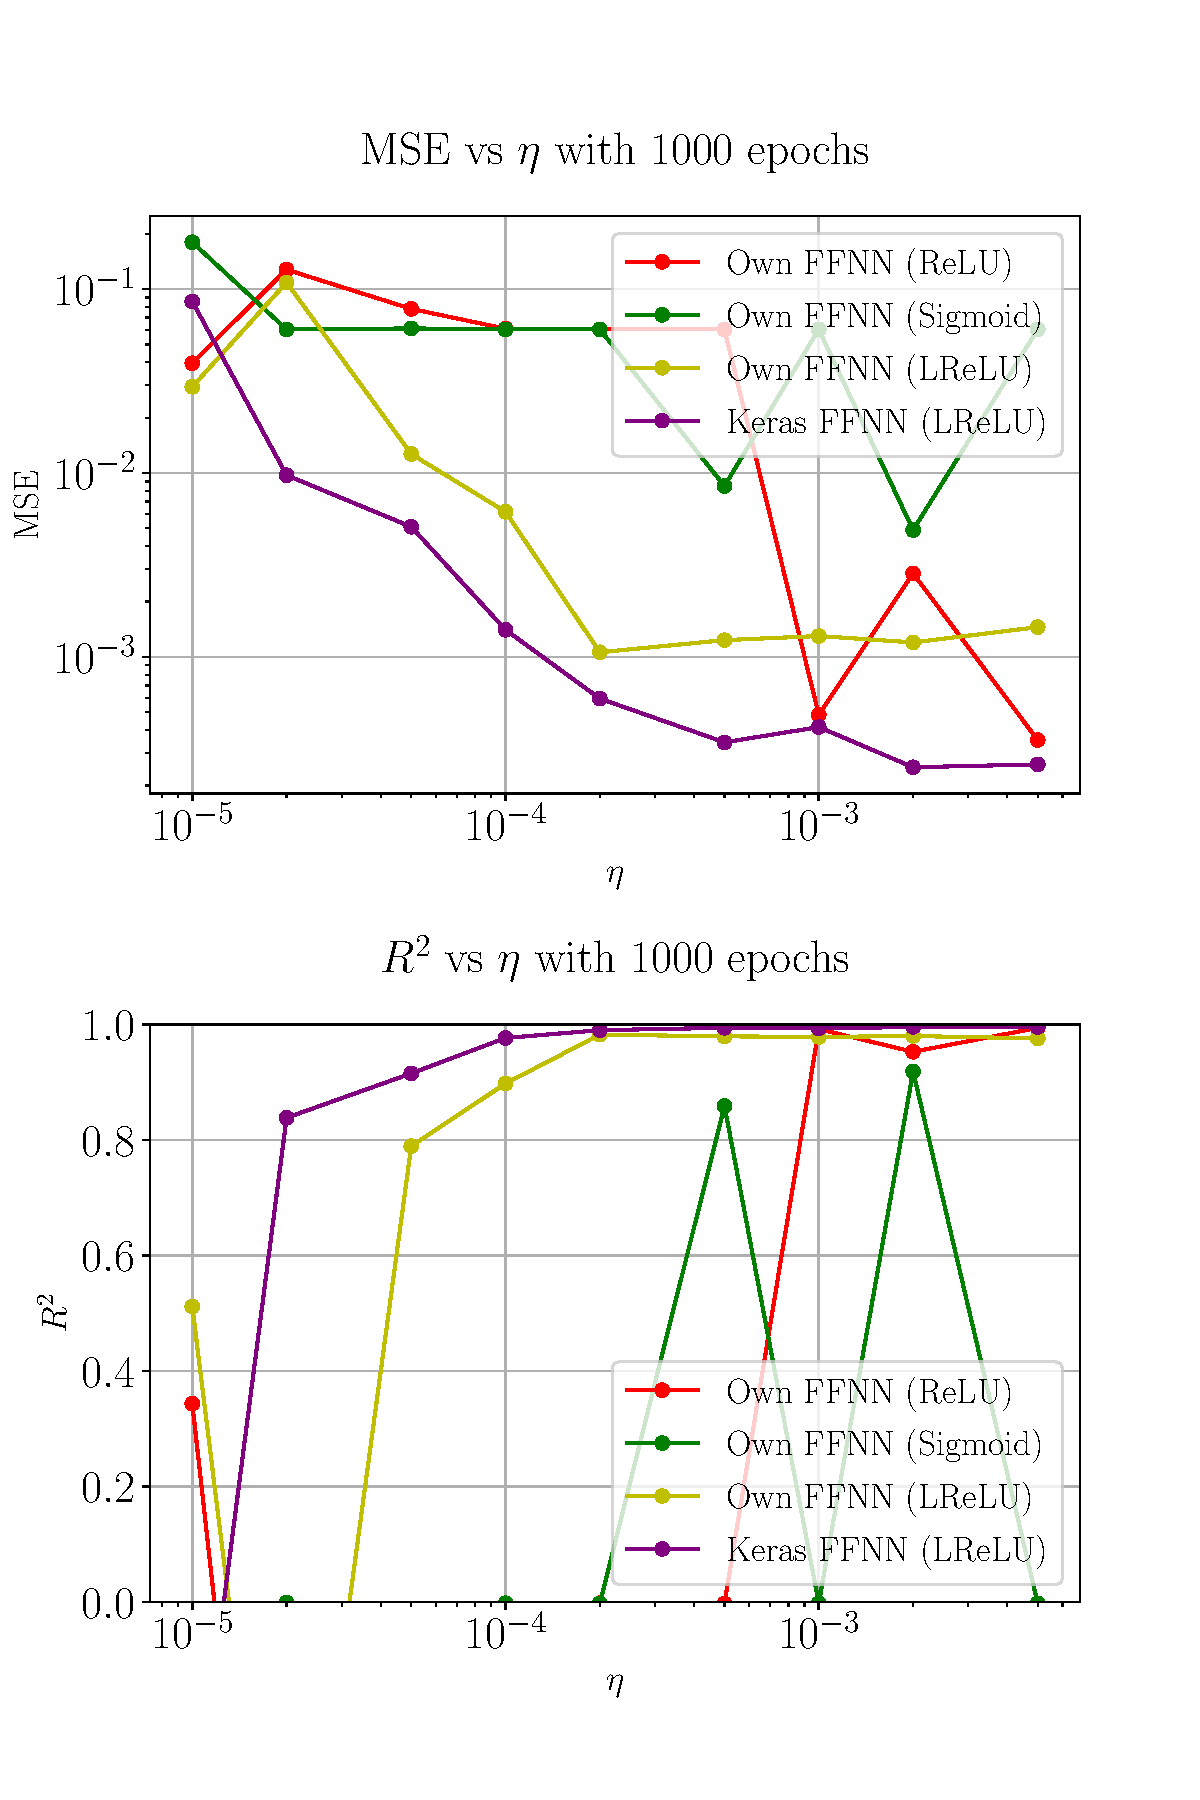
\includegraphics[width=0.5\textwidth]{Figures/NN_MSE_R2_Franke_LearningRate_Epochs1000.pdf}
	\caption{MSE and $R^2$ regression results for the FFNN as a function of $\eta$ with 1000 epochs.}
	\label{fig:NN_Franke_LR_1000}
\end{figure}

Further we used the result for the best learning rate to plot the training loss after each epoch, given in Fig. \ref{fig:NN_Franke_Epochs}. Here we see that \texttt{keras} performs much better than our implementation for low epochs, but eventually our own FFNN begins to catch up. At the end, all seem to achieve a relatively good MSE as the number of epochs increase, with the exception of our own implementation of the Sigmoid function. This makes sense due to it being more suited for binary classification tasks comapred to regression.

Further we plotted the predictions of the four variants in Fig. \ref{fig:3D_Franke}. ReLU, LReLU and \texttt{keras} are all quite close to recreating the Franke function, whilst Sigmoid performs appreciably worse.
\begin{figure}[ht!]
	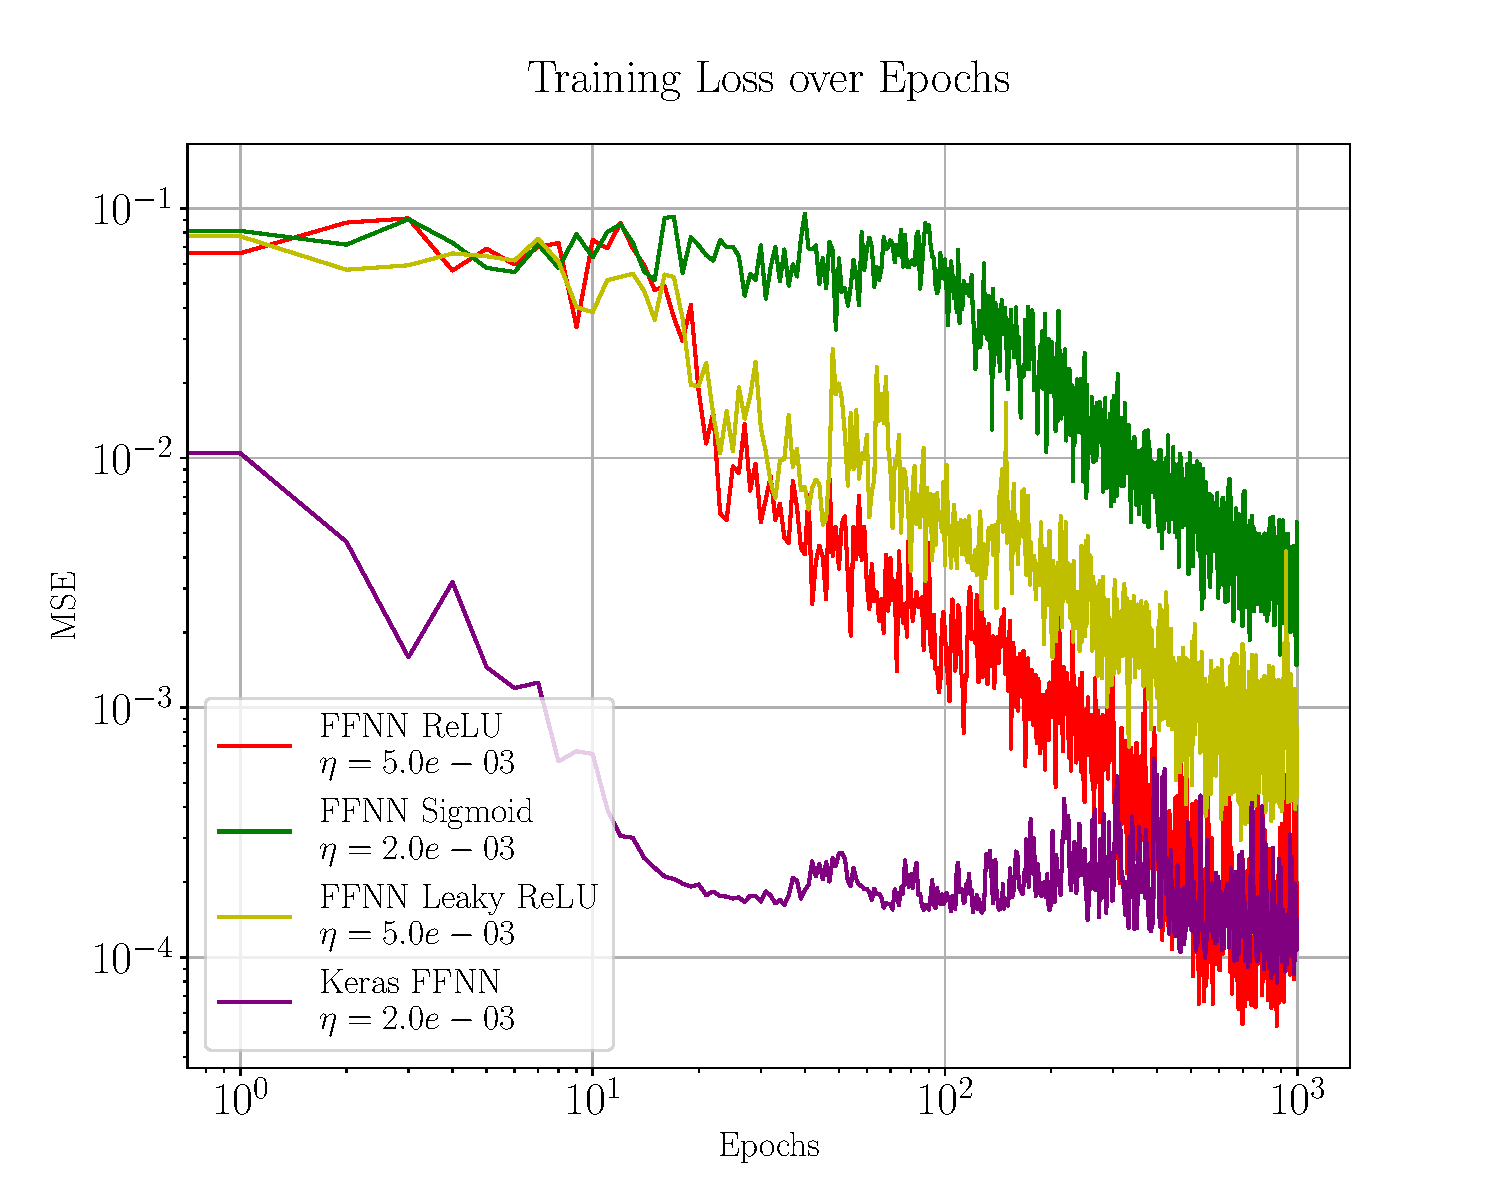
\includegraphics[width=0.5\textwidth]{Figures/NN_MSE_Franke_Epoch.pdf}
	\caption{The MSE regression results for the FFNN as a function of number of epochs for ReLU, LReLU, Sigmoid and keras.}
	\label{fig:NN_Franke_Epochs}
\end{figure}

We then did the above again, but now with a regularization parameter $\lambda$ and excluded \texttt{keras} due to time constraints. The MSE with 250 epochs for various combinations of $\eta$ and $\lambda$ are given in Fig. \ref{fig:FFNN_Franke_heatmaps}. The best results from here are then picked to once again plot the MSE over epochs given in Fig. \ref{fig:best_MSE_Franke_Epochs}. and another 3D plot to visualize the results in Fig. \ref{fig:NN_noKeras_3D_Franke_Epochs250}. Clearly the sigmoid activation function performs worse overall once again, whilst ReLU and LReLU have a close competition between them. The convergence is much faster here, and we achieve similar performance with ReLU and LReLU after only $150$ epochs. The sigmoid function converges much slower, but this is expected due to it being suited for binary classification and not regression. The much faster convergence does suggest that the regularization parameter is improving our performance significantly.
\begin{figure}[ht!]
	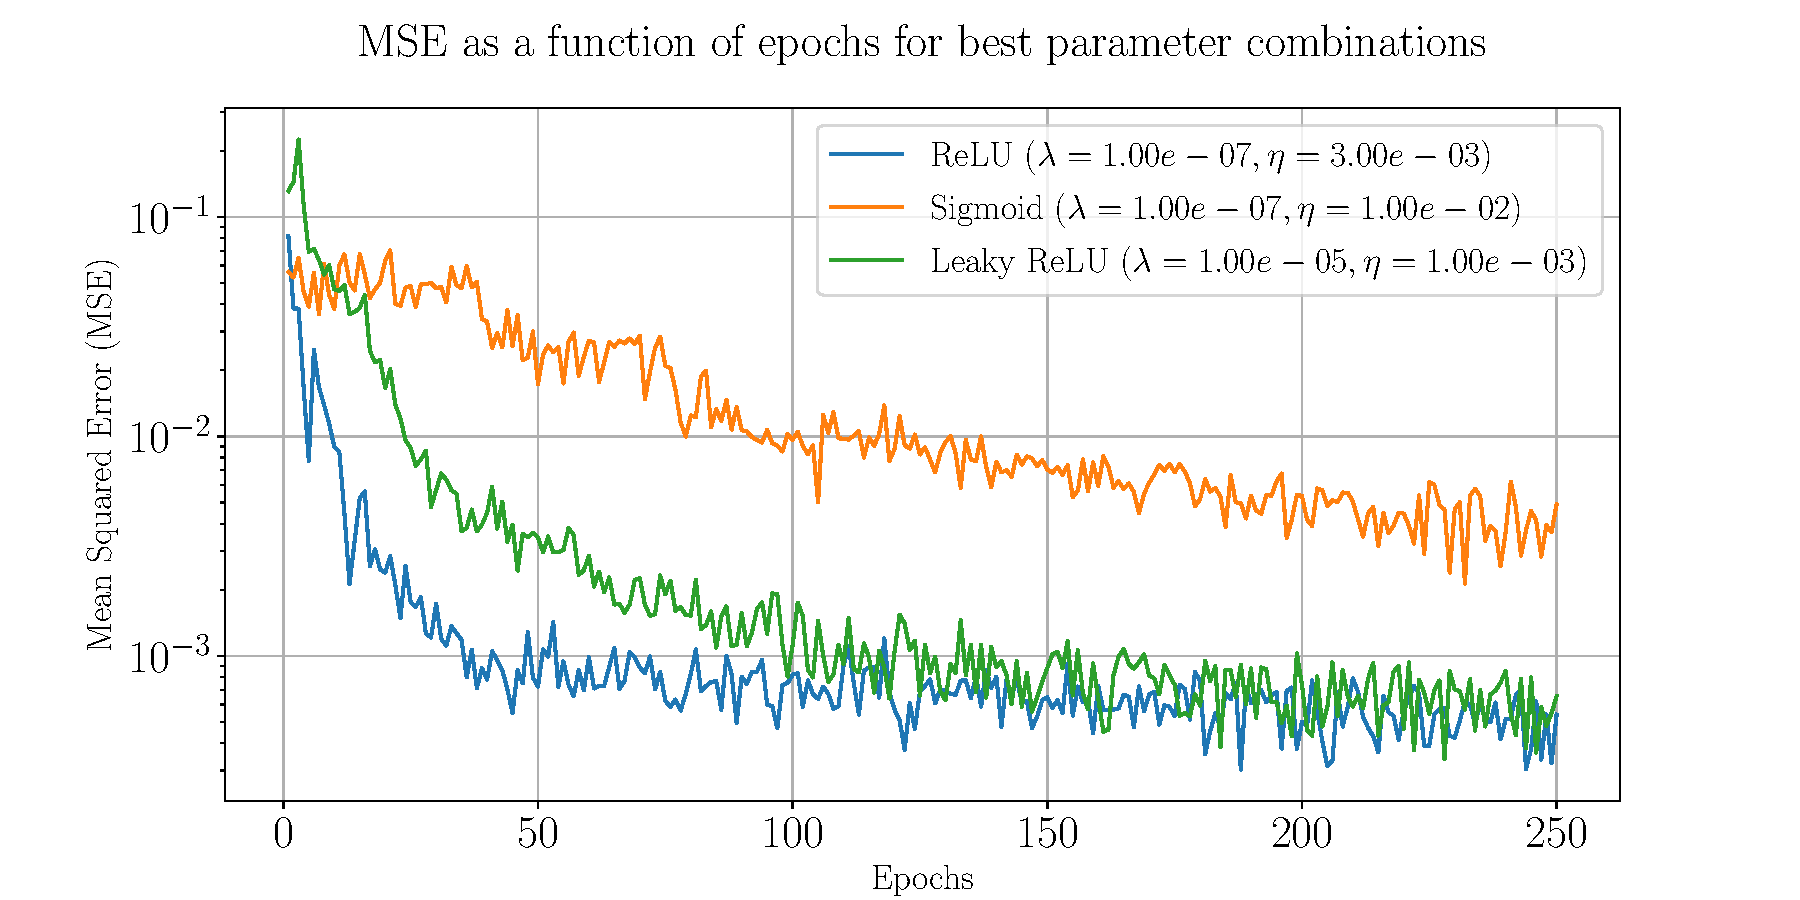
\includegraphics[width=0.5\textwidth]{Figures/Best_MSE_vs_Epochs250.pdf}
	\caption{The MSE regression results for the FFNN as a function of number of epochs for ReLU, LReLU, Sigmoid with the best performing combination of $\lambda$ and $\eta$.}
	\label{fig:best_MSE_Franke_Epochs}
\end{figure}

\subsubsection{Comparison}
From just the MSE alone we can see that the only real competition on larger number of epochs between the gradient decent methods and the FFNN is when we compare the GD methods to the Sigmoid activation function. Both the ReLU variants completely outclass all GD methods, reaching MSE scores which are an order of magnitude lower. This is of course neglecting AdaGrad which performed much worse than simply plotting the average of the Franke function, i.e. $z=0.5$, as this would give an MSE of roughly $0.066$ given our particular sample of points. Some of GD methods, in particular RMSprop and at times plain SGD, showed divergent behavior when the number of epochs was too high. In contrast, Adam continued to improve for increasing epochs, altough not as fast as FFNN. For small numbers of epoch counts, the competion between the GD methods and FFNN was more balanced; however, FFNN still came out on top in these cases as well. For the relevant low epoch FFNN figures, see \cite{extrafigures}.

\subsection{Cancer Data}
\subsubsection{Logistic Regression} \label{sec:cancer_data_logisit_regression}
Fig. \ref{fig:LogReg}. shows the accuracy score of (plain stochastic) logistic regression for batch size \(N\in\{10, 100\}\) and a batch size \(b=50\), more figures can be found in the \texttt{Figures} folder. Note that the figures to the right in Fig. \ref{fig:LogReg}. are zoomed in versions of the one to the right, and the varying learning rate has been used. This figure shows an average accuracy score of \(\sim 0.97\) for \(t_1 = 2/\eta_{\text{const}} \sim[10^{-2}, 10^{-1}]\). The more advanced optimization methods were briefly looked into, showing similar results. However, Adam diverged for \(N=100\), and AdaGrad showed promising results (accuracy scores above \(90\%\)), the opposite behavior of what we saw for linear regression. The overall best performance was found using plain SGD, keeping in mind that this was studied the most. In particular, for \(100\) epochs (and a batch size of \(50\)), the accuracy score came close to \(\sim 98\%\) for \(\lambda\sim[10^{-10}, 3.2\cdot 10^{-3}]\), \(\eta\sim[8.3\cdot 10^{-3}, 10^{-1}]\), see fig. \ref{fig:LogReg}.

\subsubsection{Neural Network}  
The accuracy of the FFNN using three activation function across different values of $\eta$ and $\lambda$ is presented in Fig \ref{fig:FFNN_cancer_heatmaps}. 

Sigmoid activation generally performs poorly across much of the parameter space, but with the right combination of $\eta$ and $\lambda$, it reaches a maximum accuracy of $97.2\%$, or 139/143 correct `guesses'.  ReLU demonstrates greater resilience to high $\eta$ and $\lambda$ values, with only certain areas of the parameter space performing poorly and a maximal accuracy of $97.9\%$. LReLU, however, achieves both the highest accuracy of $98.6\%$ and consistently performs well across almost the entire parameter range. 

Fig. \ref{fig:Confusion_FFNN} shows a confusion matrix, which illuminates where the NN failed on their best runs. We see that all 3 only fail by giving false positives. This was assumed to be due to a few difficult outliers in the test data, or lack of similar cases in the test data. We then ran the test again with a different random state on the \texttt{train\_test\_split} function, and now all the 3 activation functions all managed to get $99.3\%$ accuracy, with only one false positive on all three.

Overall it seems that ReLU and LReLU handle a wider range of learning rates and regularization strengths more effectively, likely because their piecewise linear nature prevents gradient vanishing issues, which often affect Sigmoid under aggressive learning rates. This shows the importance of choosing the right activation function for each task. 

Additionally, inputs to the Sigmoid function were clipped to prevent overflow, which might have impacted its accuracy. The slightly higher accuracy of LReLU over ReLU suggests it may provide an advantage by maintaining small gradients for negative inputs, offering a more stable training process. However, this difference, amounting to just one correct guess, may simply reflect statistical variance.

\begin{figure*}[b]
	\begin{subfigure}{0.325\textwidth}
		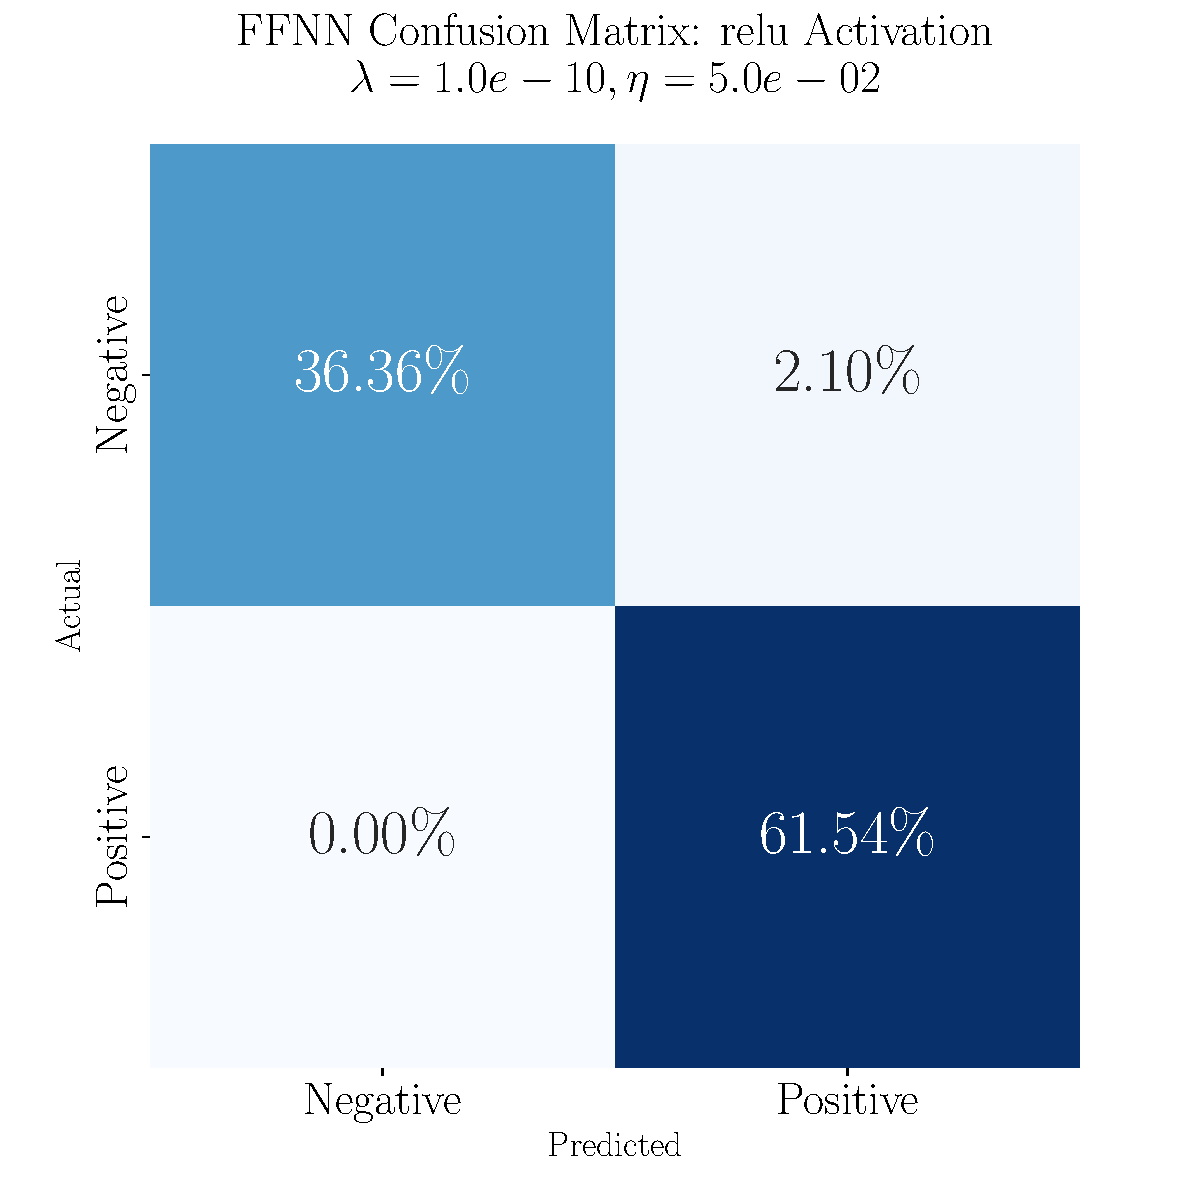
\includegraphics[width=\textwidth]{Figures/ConfusionMatrixFFNN_relu_Epochs100_randomstate1.pdf}
	\end{subfigure}
	\hfill
	\begin{subfigure}{0.325\textwidth}
		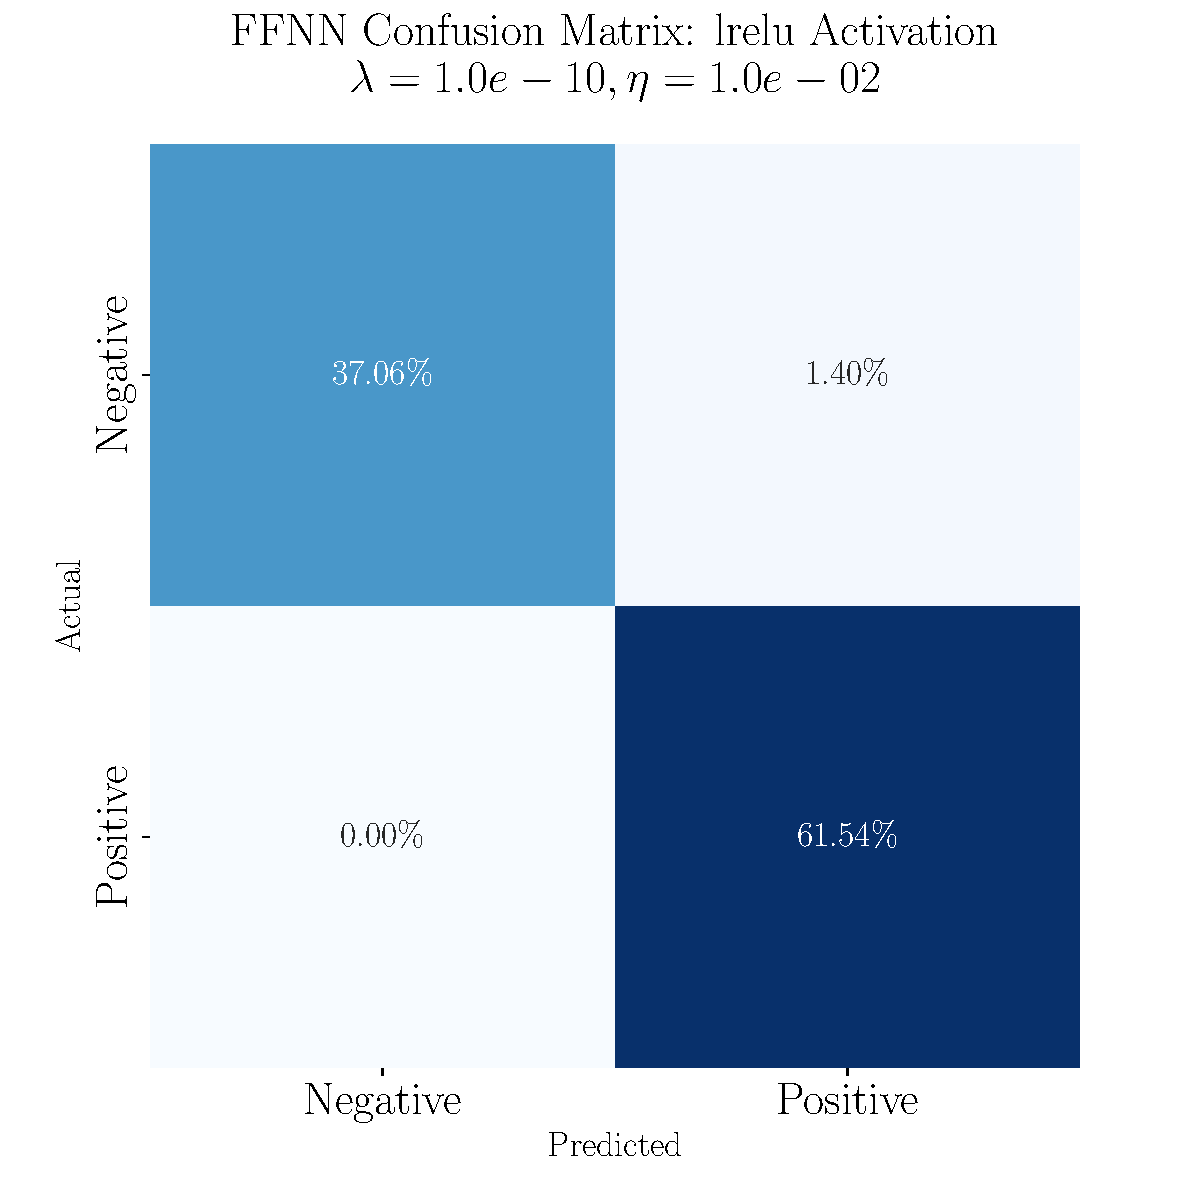
\includegraphics[width=\textwidth]{Figures/ConfusionMatrixFFNN_lrelu_Epochs100_randomstate1.pdf}
	\end{subfigure}
	\hfill
	\begin{subfigure}{0.325\textwidth}
		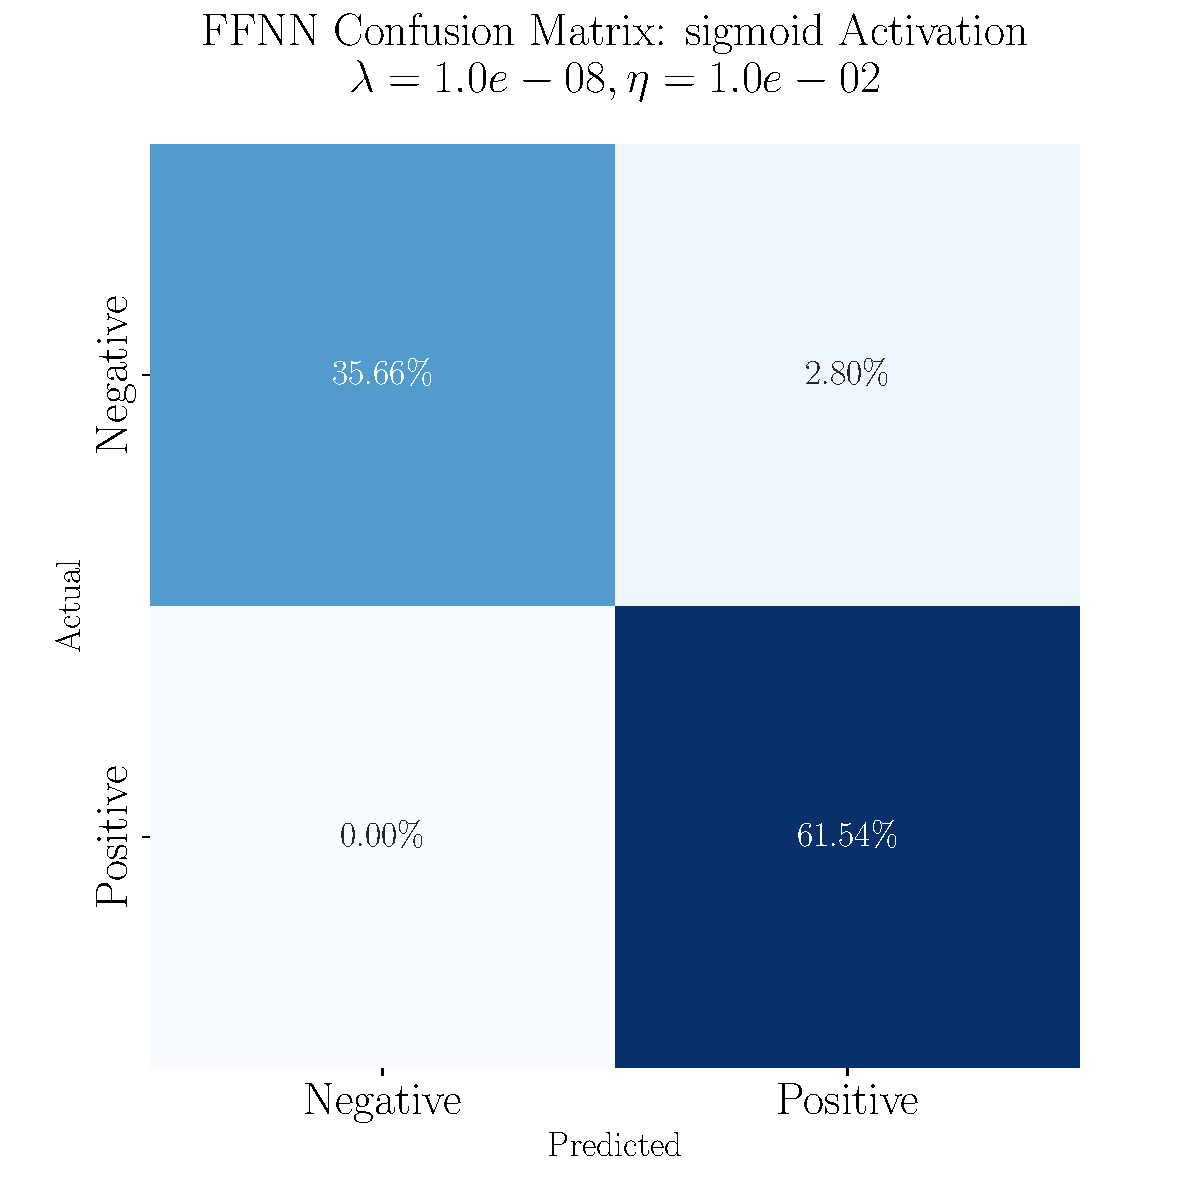
\includegraphics[width=\textwidth]{Figures/ConfusionMatrixFFNN_sigmoid_Epochs100_randomstate1.pdf}
	\end{subfigure}
	\caption{Confusion matrix of the FFNN results with 100 epochs and optimal $\eta$ and $\lambda$. The vertical axis show the correct answer, whilst the horizontal axis shows the FFNN's guess for all 3 activation functions. Perfectly guessing everything right would result in the off diagonals being $0\%$.}
	\label{fig:Confusion_FFNN}
\end{figure*}

\subsubsection{Comparison}
When comparing the results from the GD methods to the neural networks (NNs), both methods demonstrates the ability to reach high accuracies, with SGD peaking at \(\sim 98\%\) and the NNS with ReLU or LReLU achieving relatively higher scores. Both methods showed a clear dependence on the learning rate \(\eta\), and the hyperparameter \(\lambda\). Additionally, both approaches occasionally encountered convergence issues, with the Adam optimization method diverging for large batch sizes, and the neural networks showed performance variability when using the sigmoid function, especially for higher learning rates. 

The primary difference between the GD methods and the NNs, were the overall better performance of the NNs toghether with a better flexibility in their parameter space. This difference was especially noticable when using ReLU and LReLU activations, suggesting that may better handle various parameter values without suffering from issues like gradient vanishing, which can often be a problem for GD methods.

\section{Conclusion}
On the Franke function, we found that Sigmoid is not overly sensitive to changes in the learning rate and hyperparameter $\lambda$, but also struggles to find good results. On the other hand ReLU has the ability to get great results, but only for very specific combinations of $\eta$ and $\lambda$. LReLU seems to be the best of both worlds, being relatively insensitive to getting the exact right combination of $\eta$ and $\lambda$, whilst still managing to obtain very good MSE scores like ReLU. When comparing the MSE scores to the MSE scores of the GD methods, we found that the NNs, in particular those utilizing ReLU and LReLU, consistently delivered an overall better performance. The best performing GD method; Adam showed convergence for various different parameters, and lower MSE scores compared to those of plain SGD,  AdaGrad and RMSprop. However, they were still outperformed by the FFNN. In particular, for increasing epochs, the NNs performance consistently increased, a trend which only Adam shared, though with lower metric scores.

For the FFNN on the cancer data, overall assessments here are similar for the Franke function. The best perfoming activation function was again LReLU, followed by ReLU and finally the Sigmoid function. The latter performed much better on this classification problem compared to regression as one would expect from its definition, but once again still falls short to the ReLU variants. At its best, the FFNN gave accuracy scores of about \(99\%\), beating plain SGD at \(\sim 98\%\). 

There are plentiful of avenues to pursue which can extend and improve our analysis. A simple example would be testing out different values of $\alpha$ in LReLU and seeing whether it may achieve an even higher level of performance. Similarly, we never adjusted $\beta_1$ and $\beta_2$ throughout, and there is no reason to expect that our particular choices for these are the optimal values. Further, thoroughly testing out other optimizers such as Adagrad and RMSprop for the FFNN may also yield benefits, but due to time constraints we did not implement this properly. Whilst we did test different hidden layer setups, this was not done extensively. The odds of us achieving an optimal setup with relatively few attempts compared to possible combinations, is next to null. 

% Bibliography
\bibliographystyle{JHEP}
\bibliography{project2}

\appendix
\section{Large Figures}
\label{Appendix:A}
A selection of figures, more can be found in the \texttt{Figures} folder.

%%%%%%%%%%%%%% Franke %%%%%%%%%%%%%%

%%%%%%%%% Linear Regression %%%%%%%%%
\begin{figure*}
	\begin{subfigure}{0.41\textwidth}
		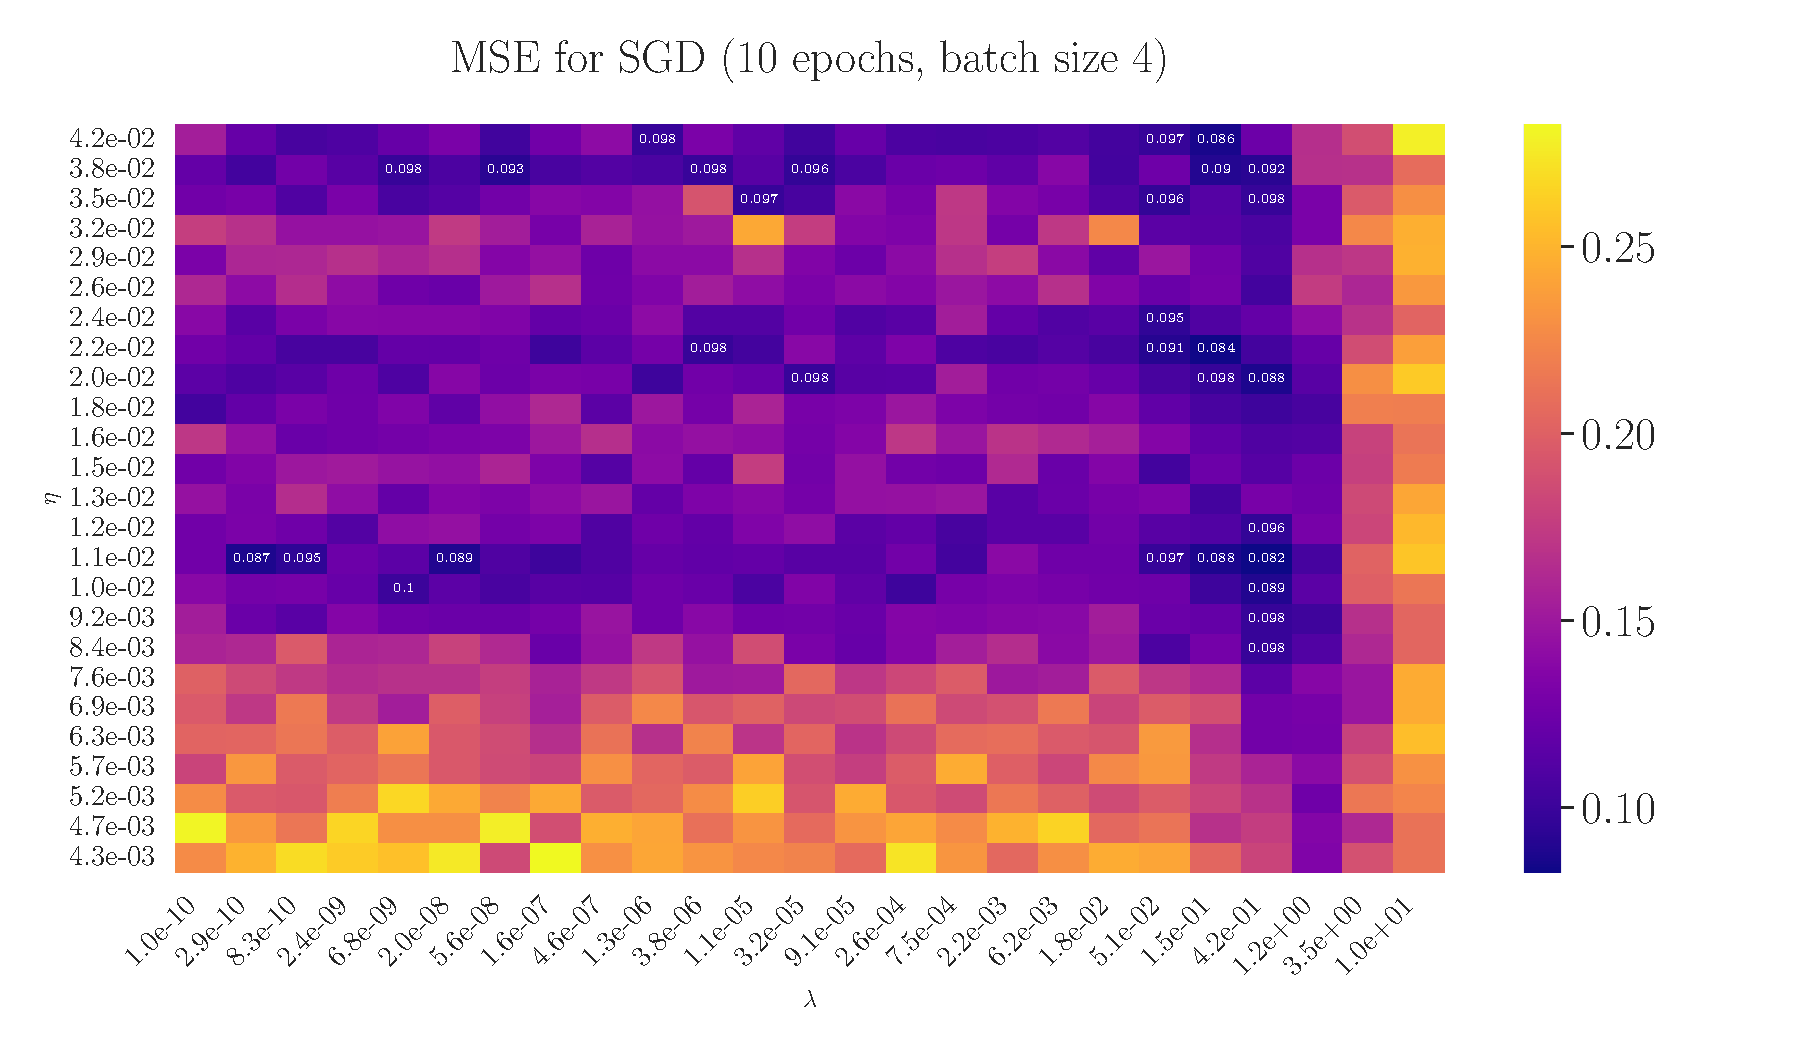
\includegraphics[width=\textwidth]{Figures/LinRegSGD_25x25_epoch10_batchS4.pdf}
		\caption{MSE score using SGD for franke data.}
		\label{fig:LinReg25x25_epoch10_bacthS50}
	\end{subfigure}
	\hfill
	\begin{subfigure}{0.41\textwidth}
		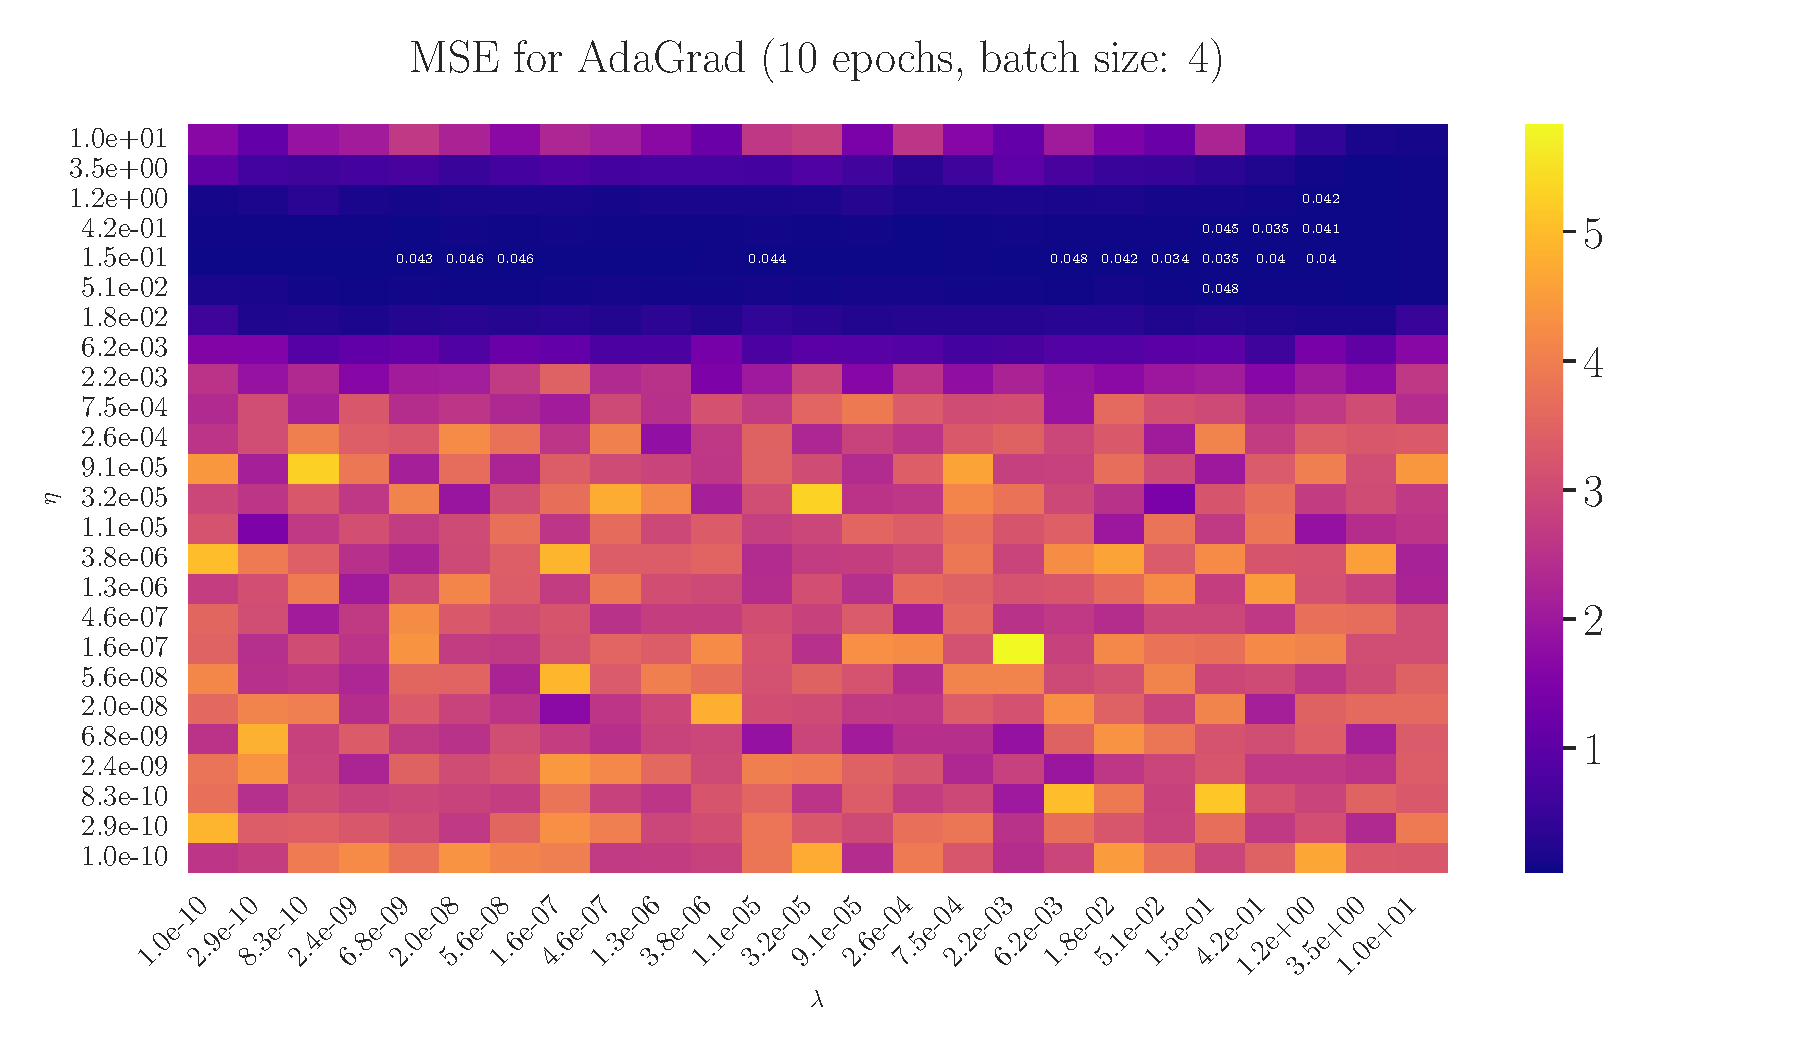
\includegraphics[width=\textwidth]{Figures/LinRegAdaGrad_25x25_epoch10_batchS4.pdf}
		\caption{MSE score using AdaGrad for franke data.}
		\label{fig:LinReg25x25_epoch10_bacthS50_zoomed}
	\end{subfigure}
\hfill\newline
	\begin{subfigure}{0.41\textwidth}
		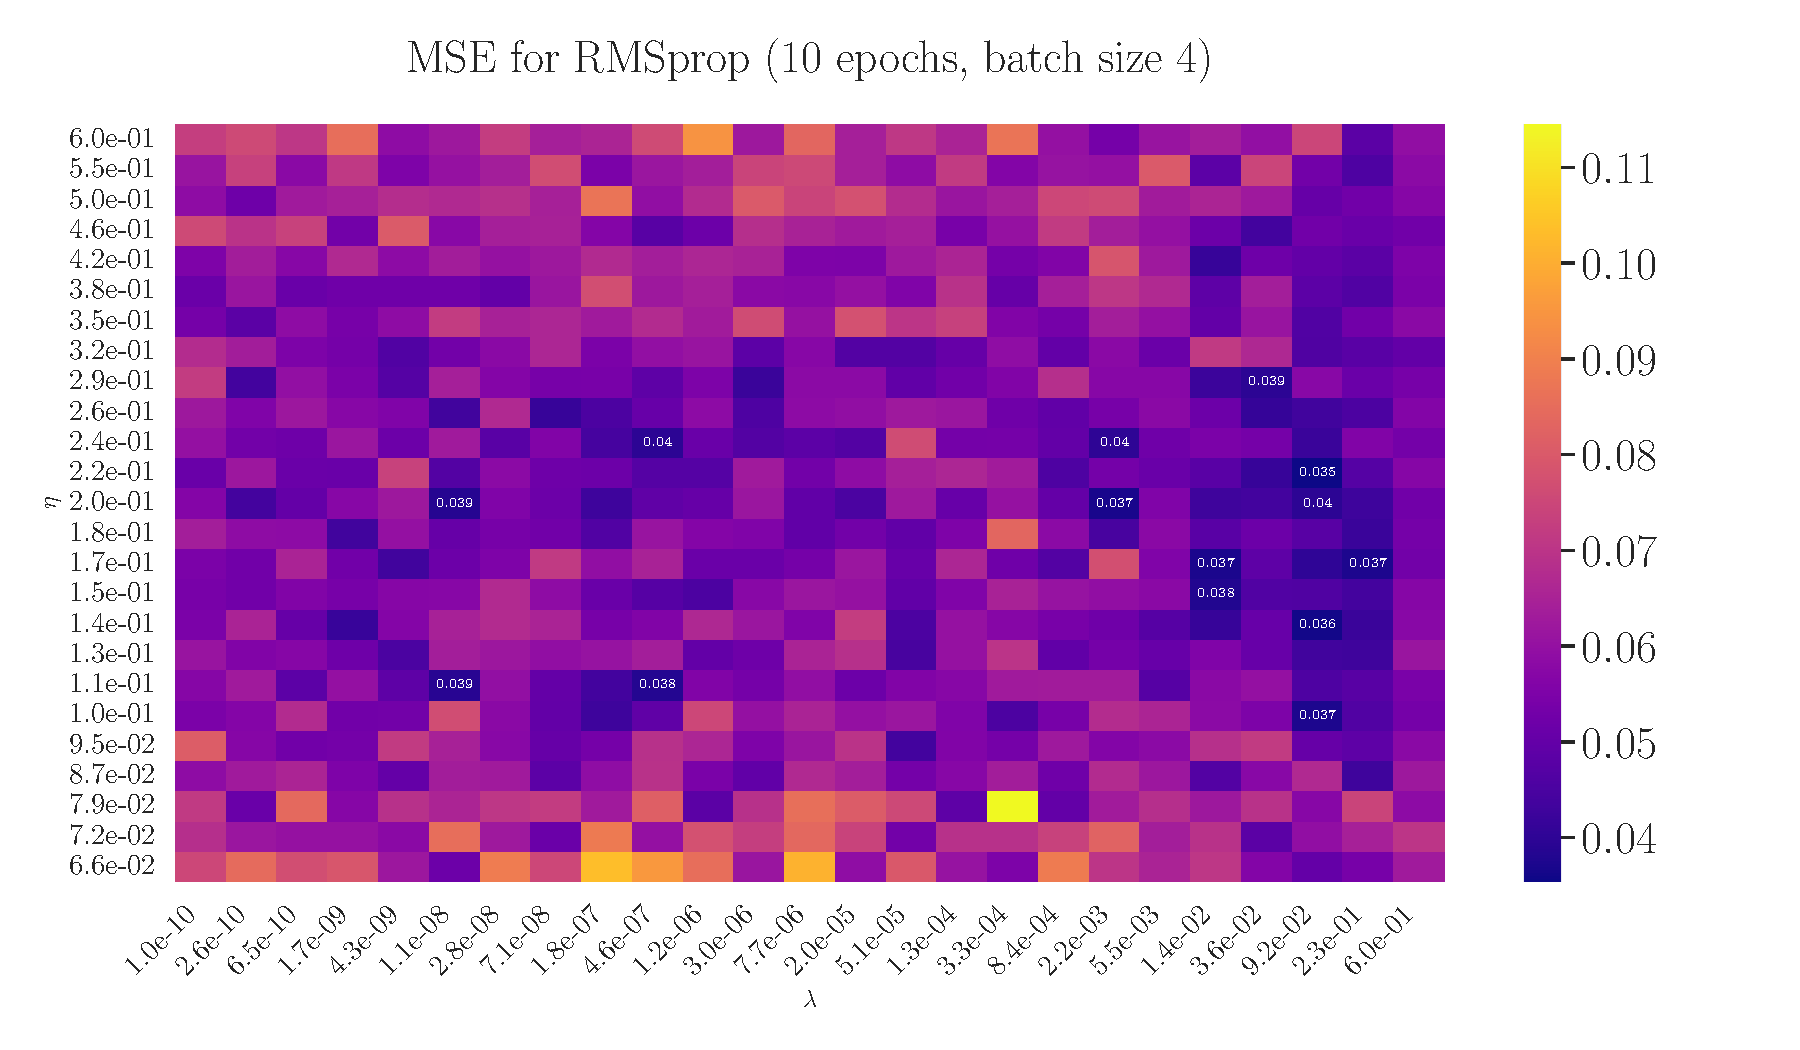
\includegraphics[width=\textwidth]{Figures/LinRegRMSprop_25x25_epoch10_batchS4.pdf}
		\caption{MSE score using RMSprop for franke data.}
		\label{fig:LinReg25x25_epoch100_bacthS50}
	\end{subfigure}
	\hfill
	\begin{subfigure}{0.41\textwidth}
		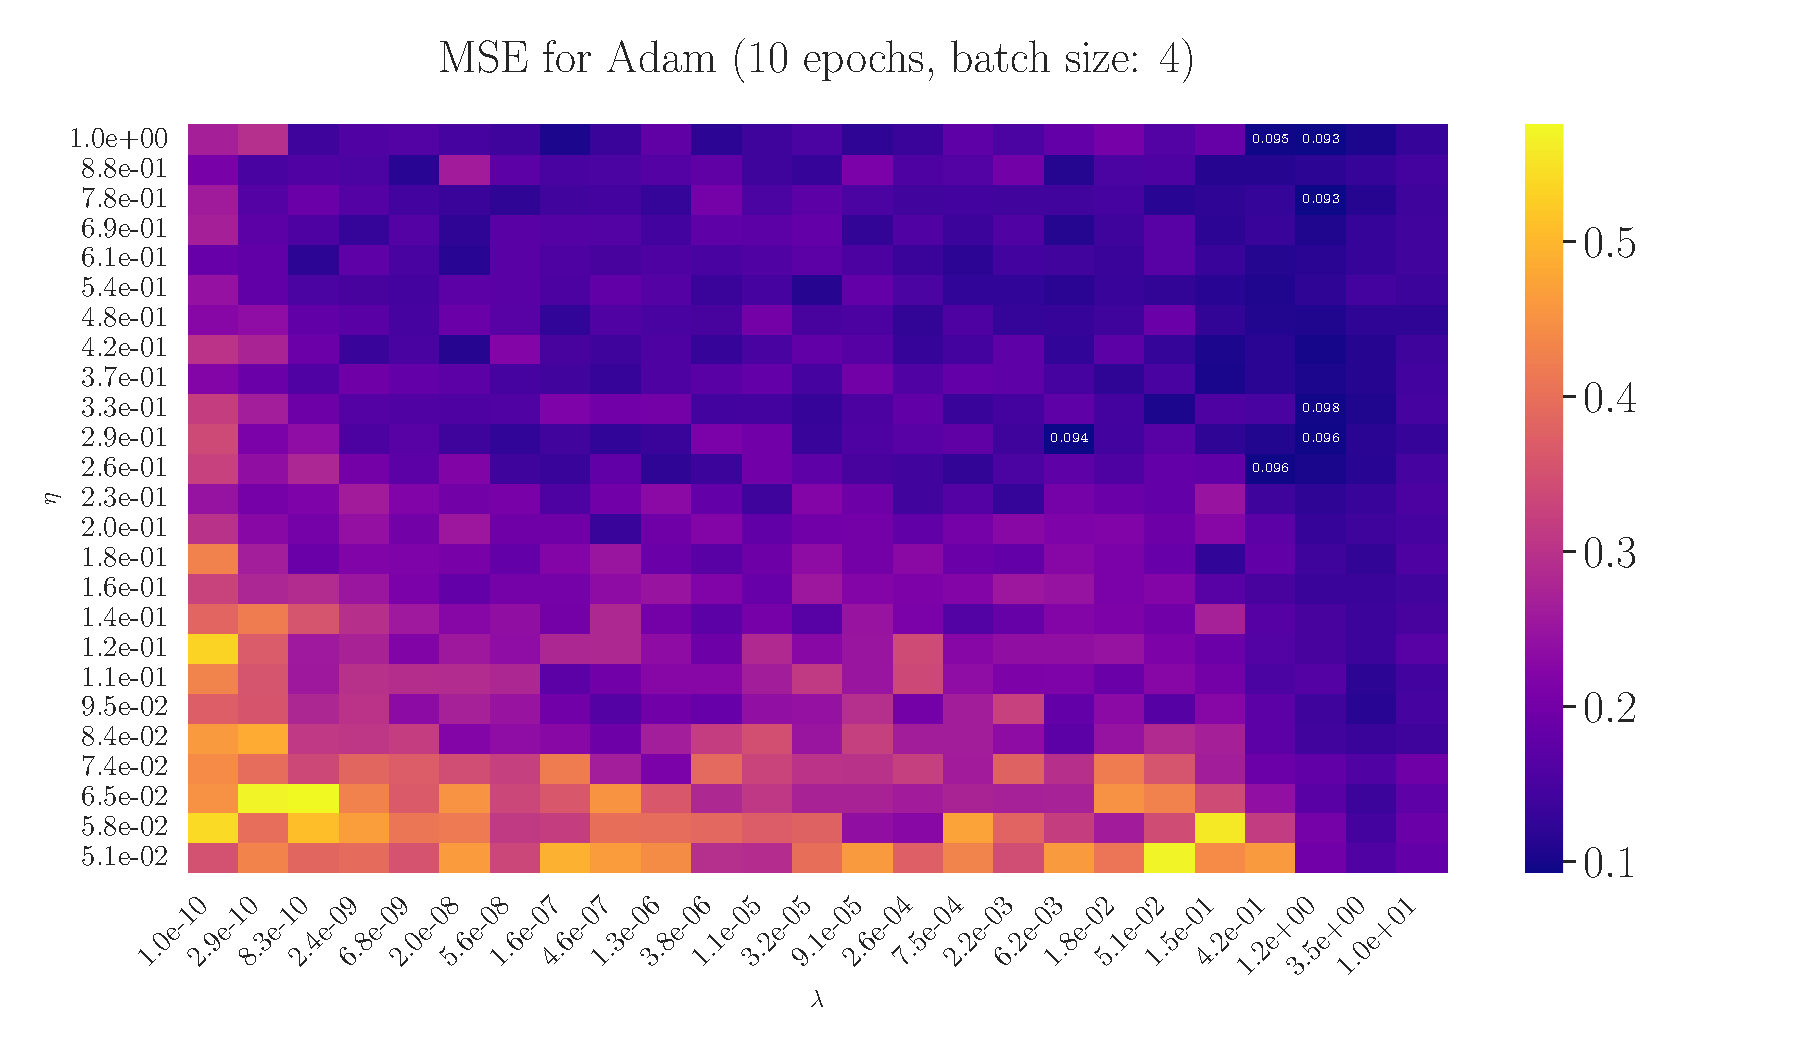
\includegraphics[width=\textwidth]{Figures/LinRegAdam_25x25_epoch10_batchS4_zoomed.pdf}
		\caption{MSE score using Adam for franke data.}
		\label{fig:LinReg25x25_epoch100_bacthS50_zoomed}
	\end{subfigure}
	\caption{MSE scores for linear regression on \(20\) data samples from the Franke function, for number of epochs \(N=10\) and a batch size of \(4\). A varying learning rate is used, and the \(y\)-axis denotes \(\eta_{\text{const}}\), which is used to set \(t_1\) in \eqref{eq:varyin_learning_rate}.}
	\label{fig:LinReg}
\end{figure*}

\begin{figure*}
	\begin{subfigure}{0.41\textwidth}
		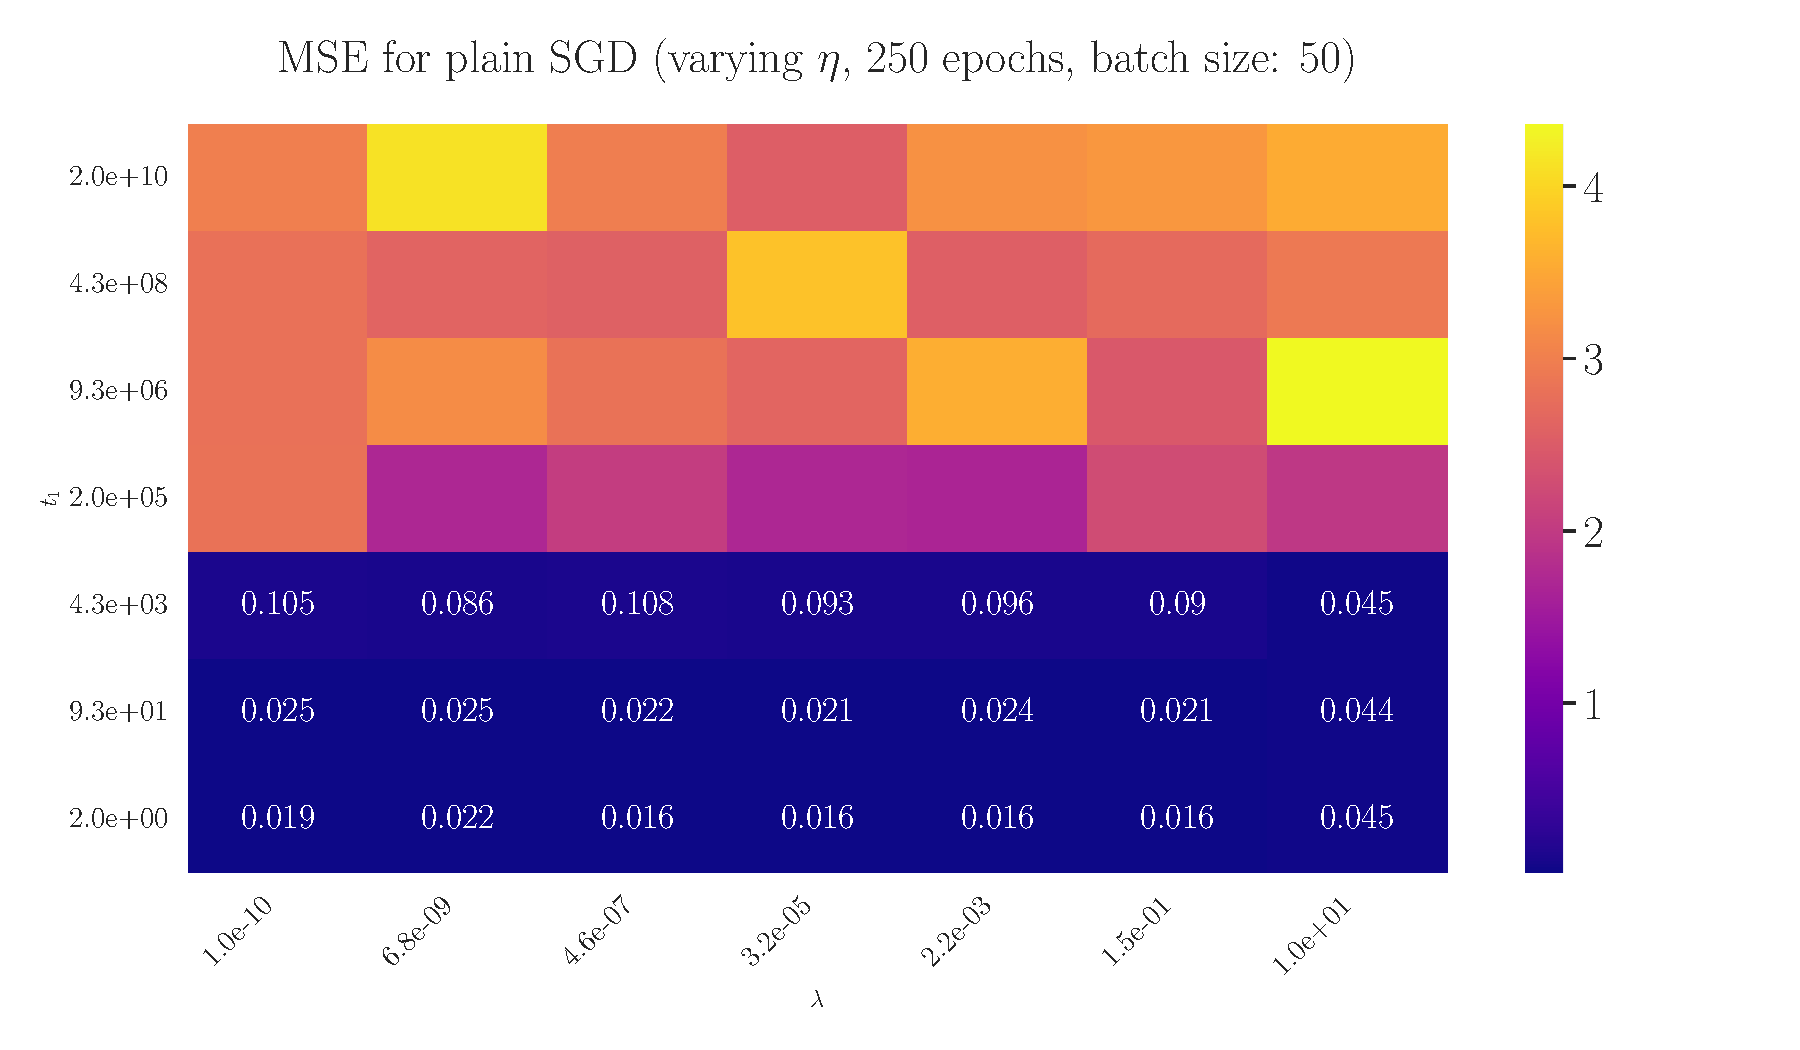
\includegraphics[width=\textwidth]{Figures/LinRegPlainSGD_250epochs_batchS50.pdf}
		\caption{MSE score using SGD for franke data.}
		\label{fig:LinReg25x25_epoch10_bacthS50}
	\end{subfigure}
	\hfill
	\begin{subfigure}{0.41\textwidth}
		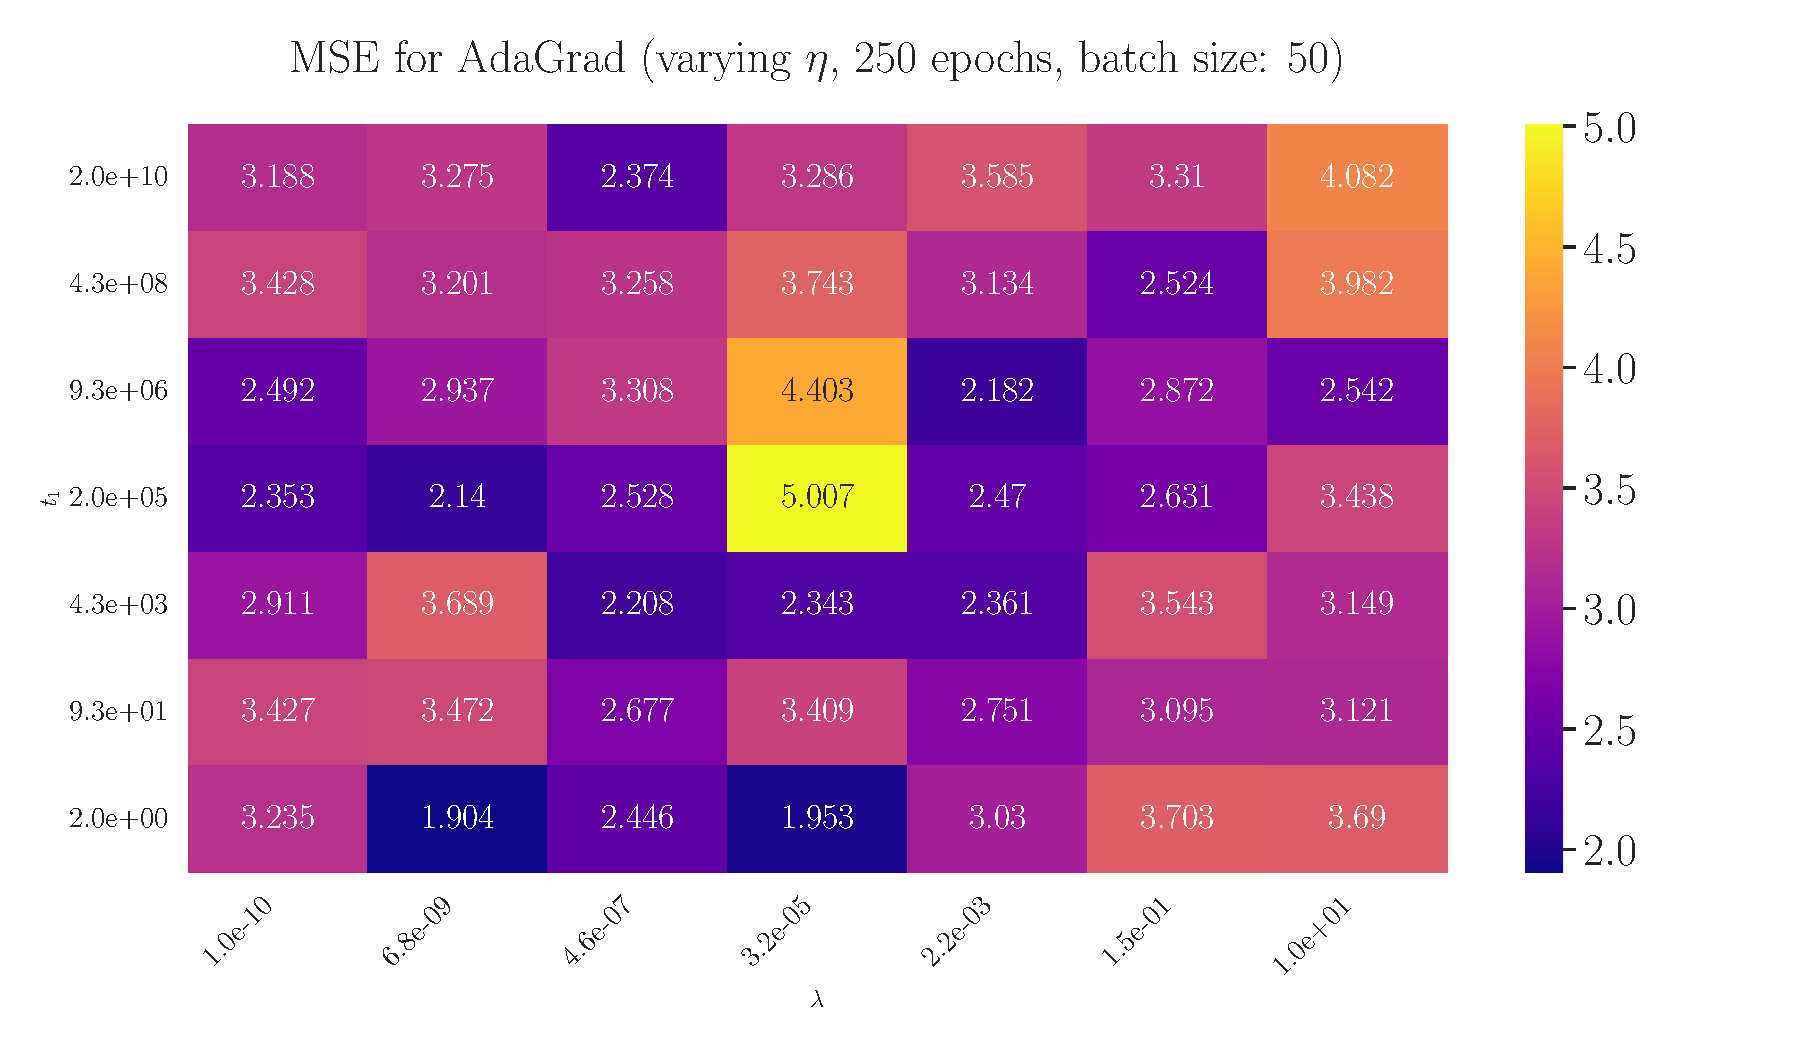
\includegraphics[width=\textwidth]{Figures/LinRegAdaGrad_250epochs_batchS50.pdf}
		\caption{MSE score using AdaGrad for franke data.}
		\label{fig:LinReg25x25_epoch10_bacthS50_zoomed}
	\end{subfigure}
\hfill\newline
	\begin{subfigure}{0.41\textwidth}
		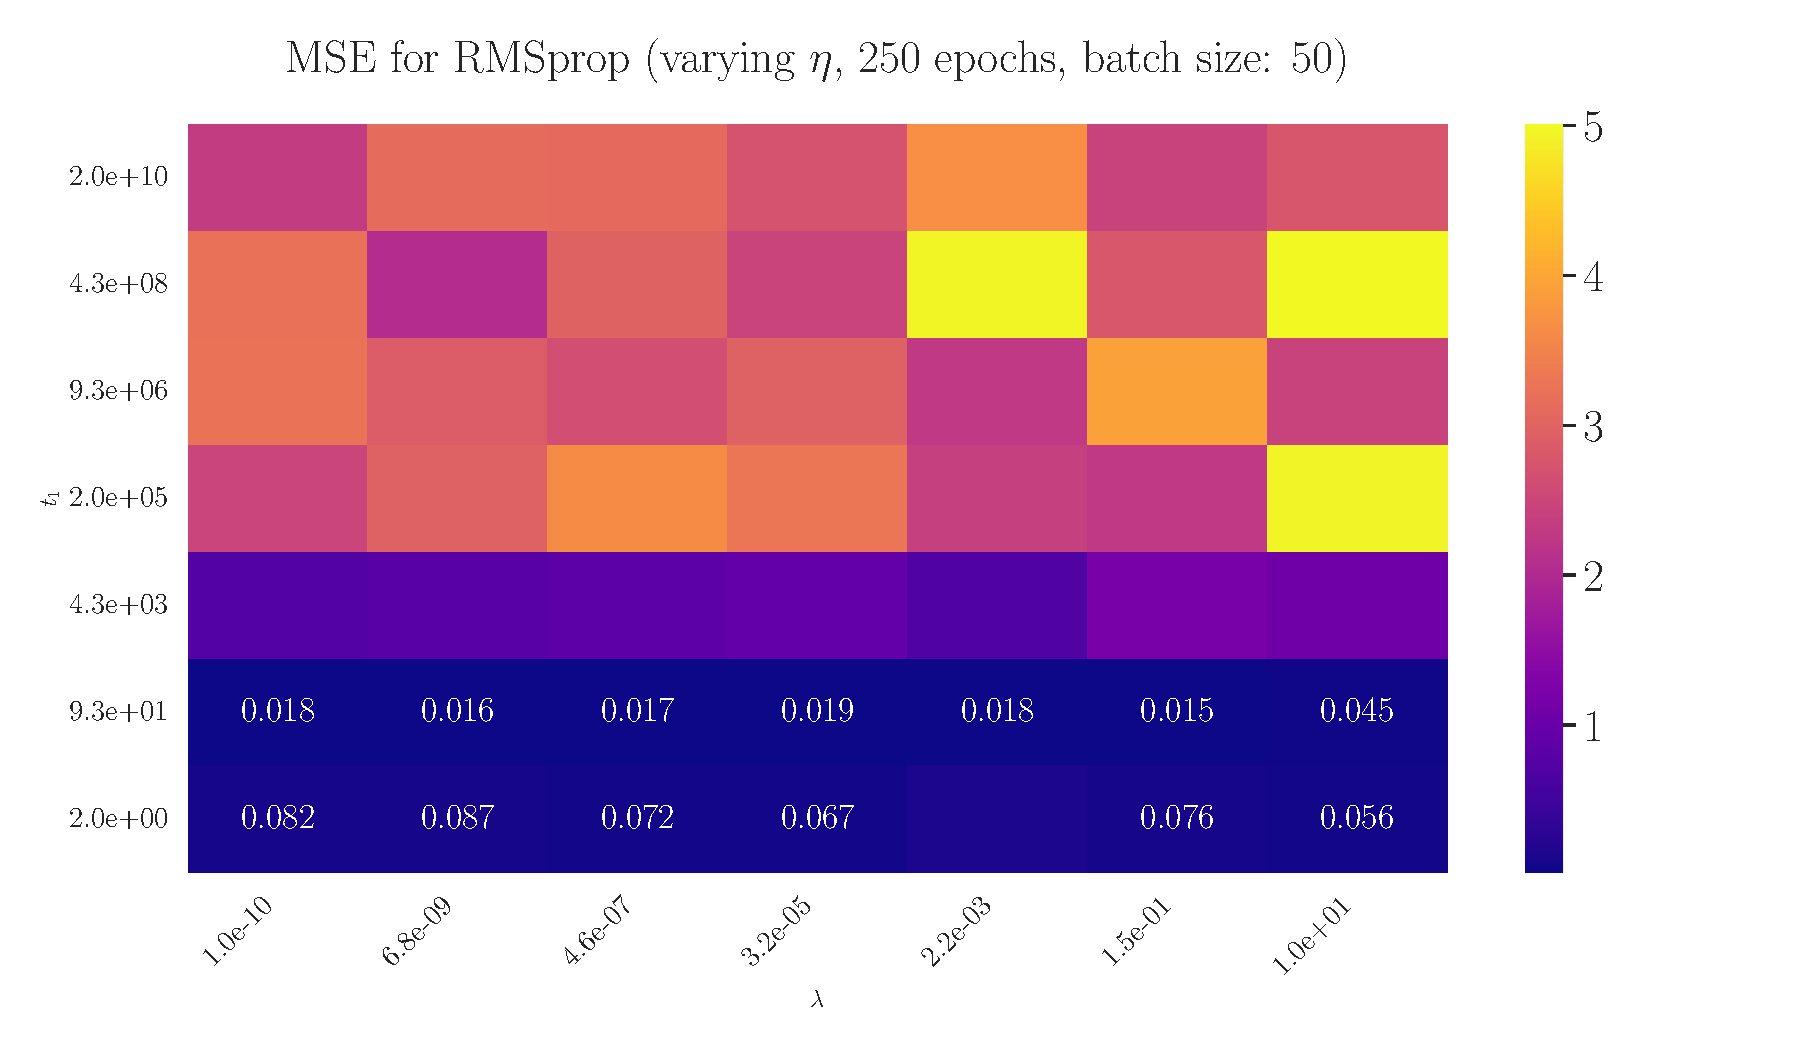
\includegraphics[width=\textwidth]{Figures/LinRegRMSprop_250epochs_batchS50.pdf}
		\caption{MSE score using RMSprop for franke data.}
		\label{fig:LinReg25x25_epoch100_bacthS50}
	\end{subfigure}
	\hfill
	\begin{subfigure}{0.41\textwidth}
		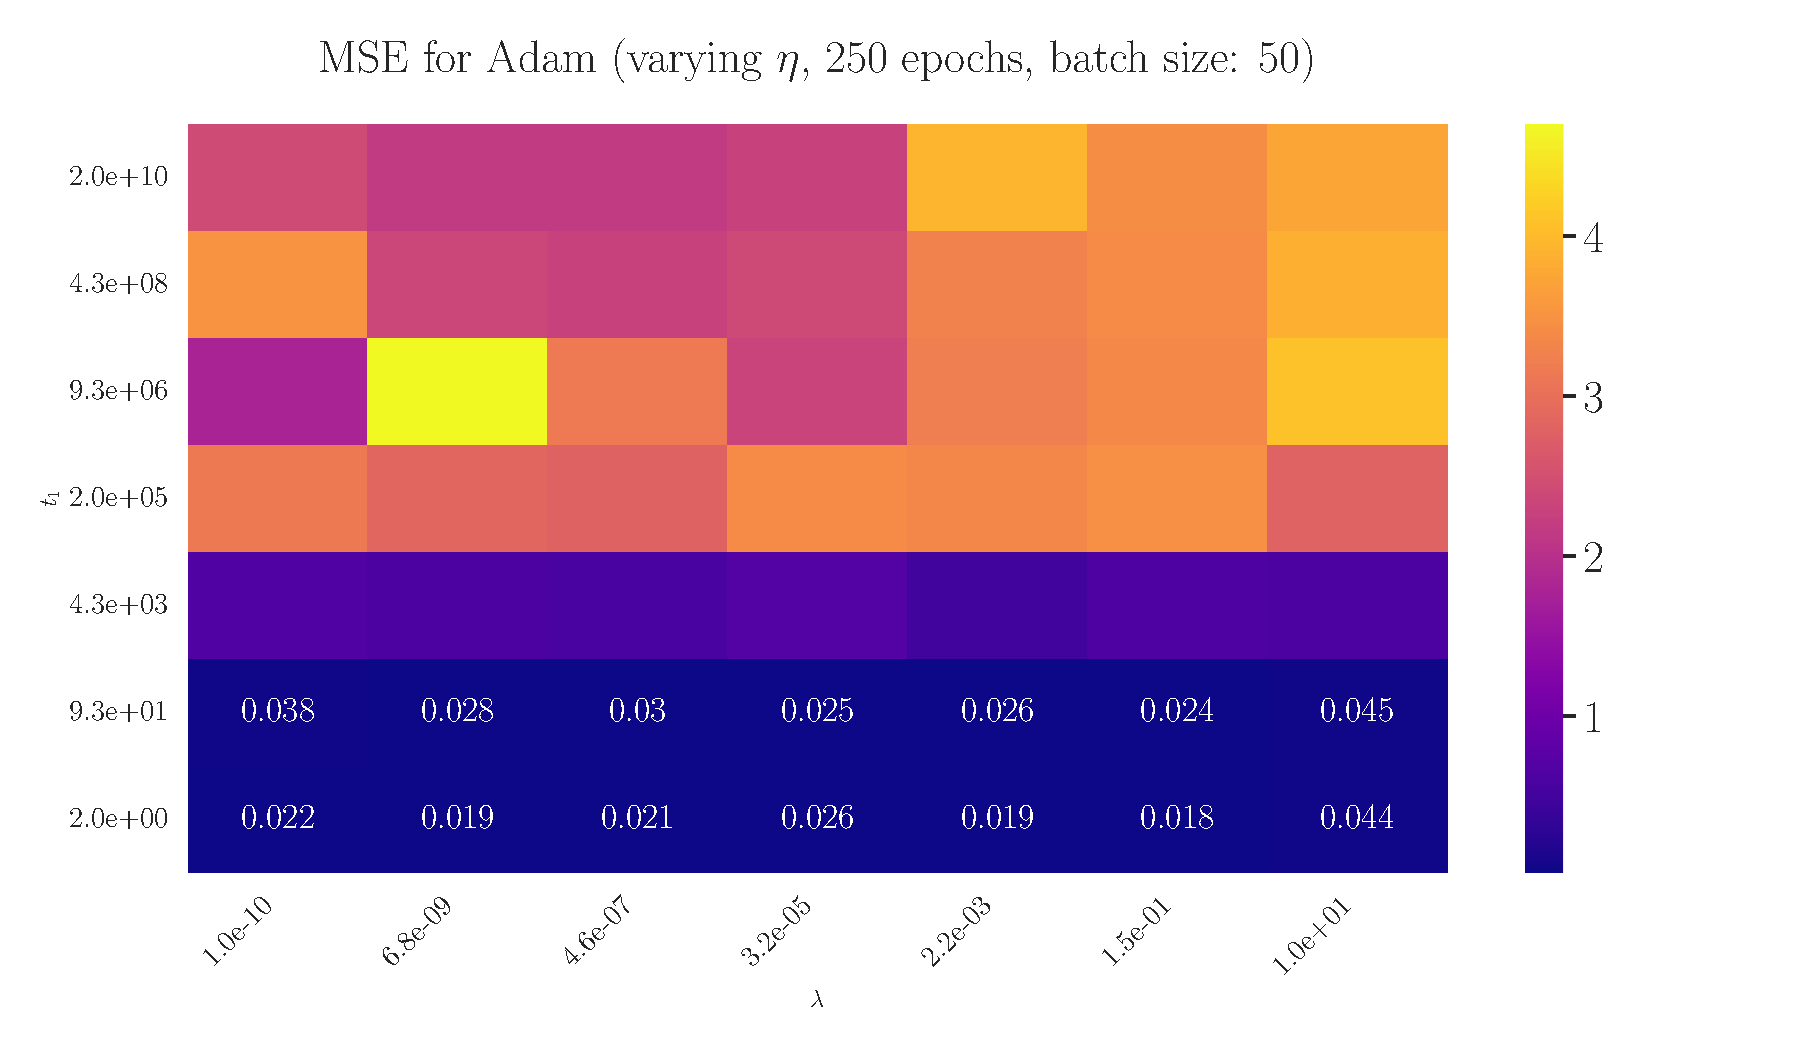
\includegraphics[width=\textwidth]{Figures/LinRegAdam_250epochs_batchS50.pdf}
		\caption{MSE score using Adam for franke data.}
		\label{fig:LinReg25x25_epoch100_bacthS50_zoomed}
	\end{subfigure}
	\caption{MSE scores for linear regression on \(250\) data samples from the Franke function, for number of epochs \(N=250\) and a batch size of \(50\). A varying learning rate is used, and the \(y\)-axis denotes \(t_1 = 2/\eta_{\text{const}}\) in \eqref{eq:varyin_learning_rate}.}
	\label{fig:LinReg_250}
\end{figure*}

%%%%%%%%% Neural Network different acitivation functions %%%%%%%%%

\begin{figure*}[ht!]
	\begin{subfigure}[b]{0.43\textwidth}
		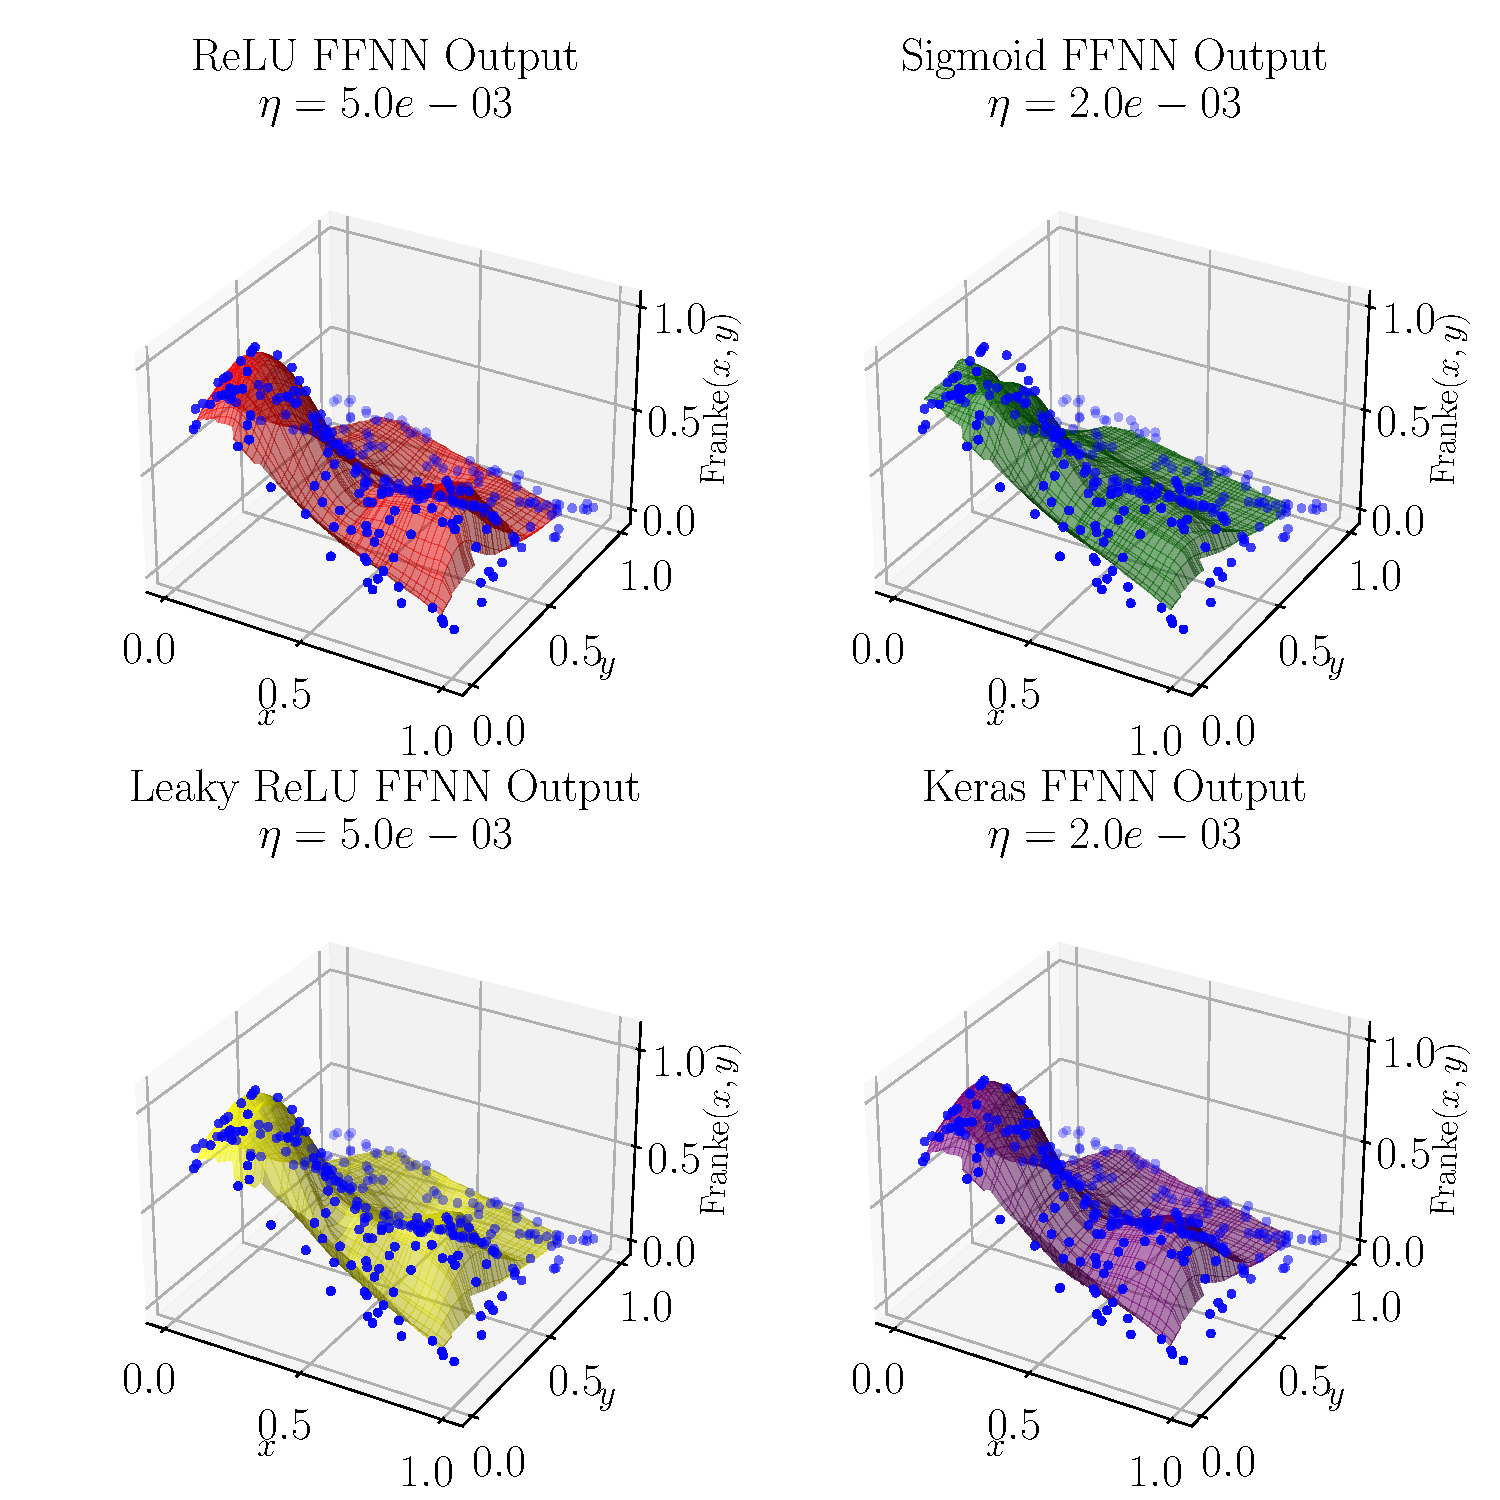
\includegraphics[width=\textwidth]{Figures/NN_3D_Predict_Franke_Epochs1000.pdf}
		\caption{3D plots for best $\eta$ with $1000$ epochs. The blue dots correspond to the sampled points from the Franke function with $250$ total samples.}
		\label{fig:3D_Franke}
	\end{subfigure}
	\hfill
	\begin{subfigure}[b]{0.43\textwidth}
		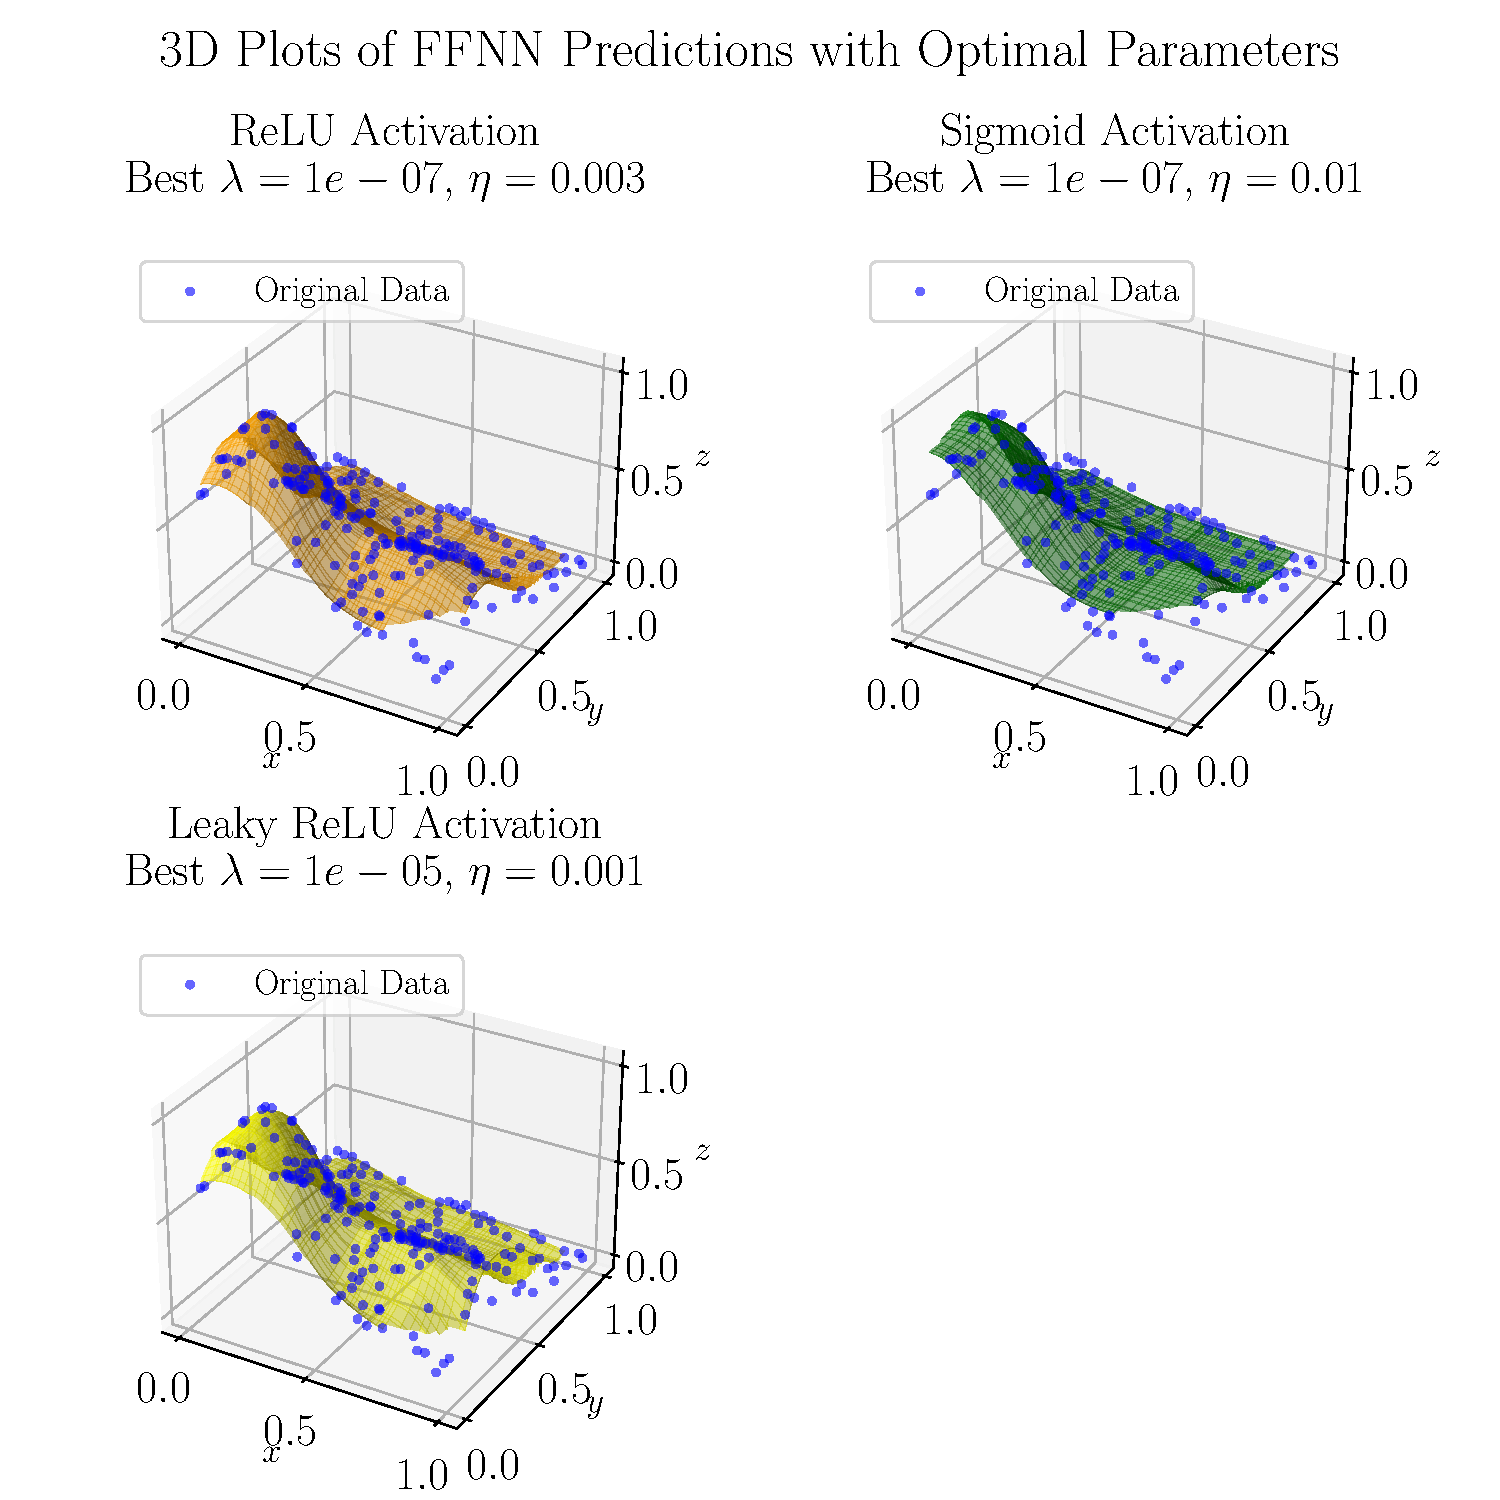
\includegraphics[width=\textwidth]{Figures/NN_noKeras_3D_Franke_Epochs250.pdf}
		\caption{3D plots for best combination of $\lambda$ and $\eta$ for our own neural network with $250$ epochs and $100$ samples from the Franke function.}
		\label{fig:NN_noKeras_3D_Franke_Epochs250}
	\end{subfigure}
\end{figure*}

\begin{figure*}[ht!]
	\begin{subfigure}{0.41\textwidth}
		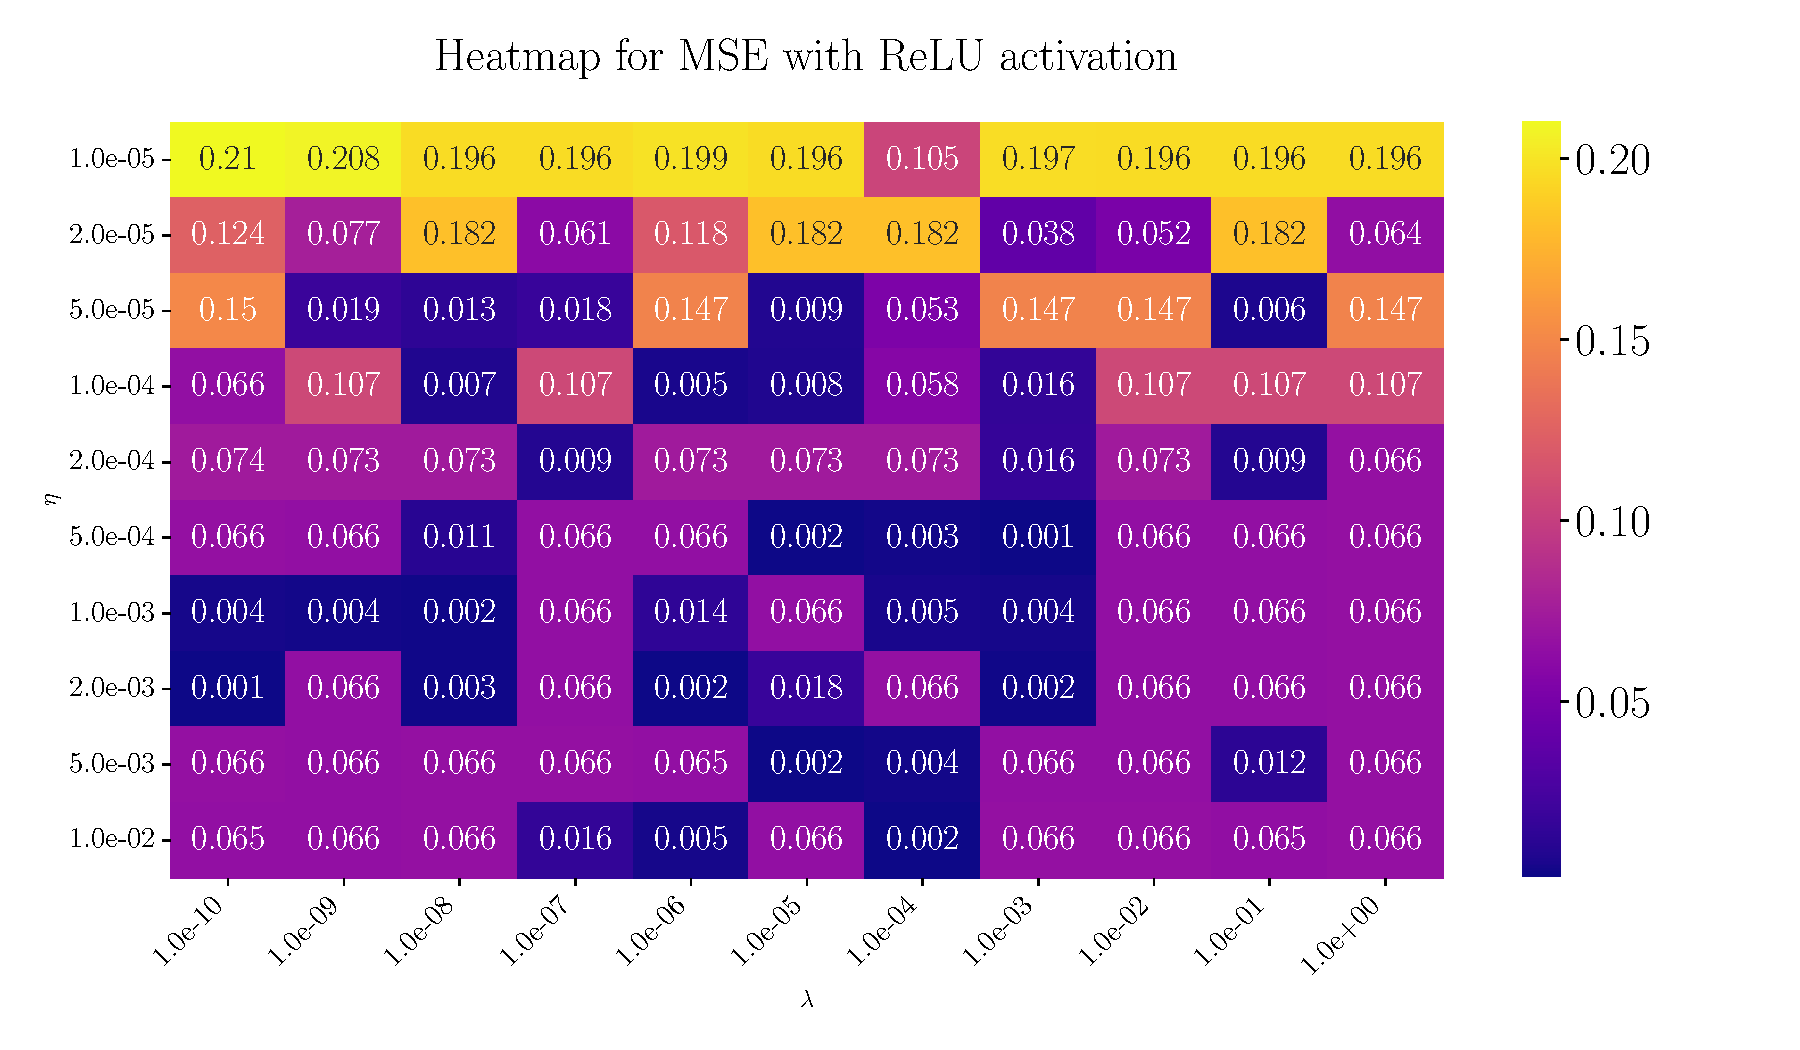
\includegraphics[width=\textwidth]{Figures/Heatmap_MSE_ReLU_Franke_Epochs250.pdf}
		\caption{ReLU}
	\end{subfigure}
	\hfill
	\begin{subfigure}{0.41\textwidth}
		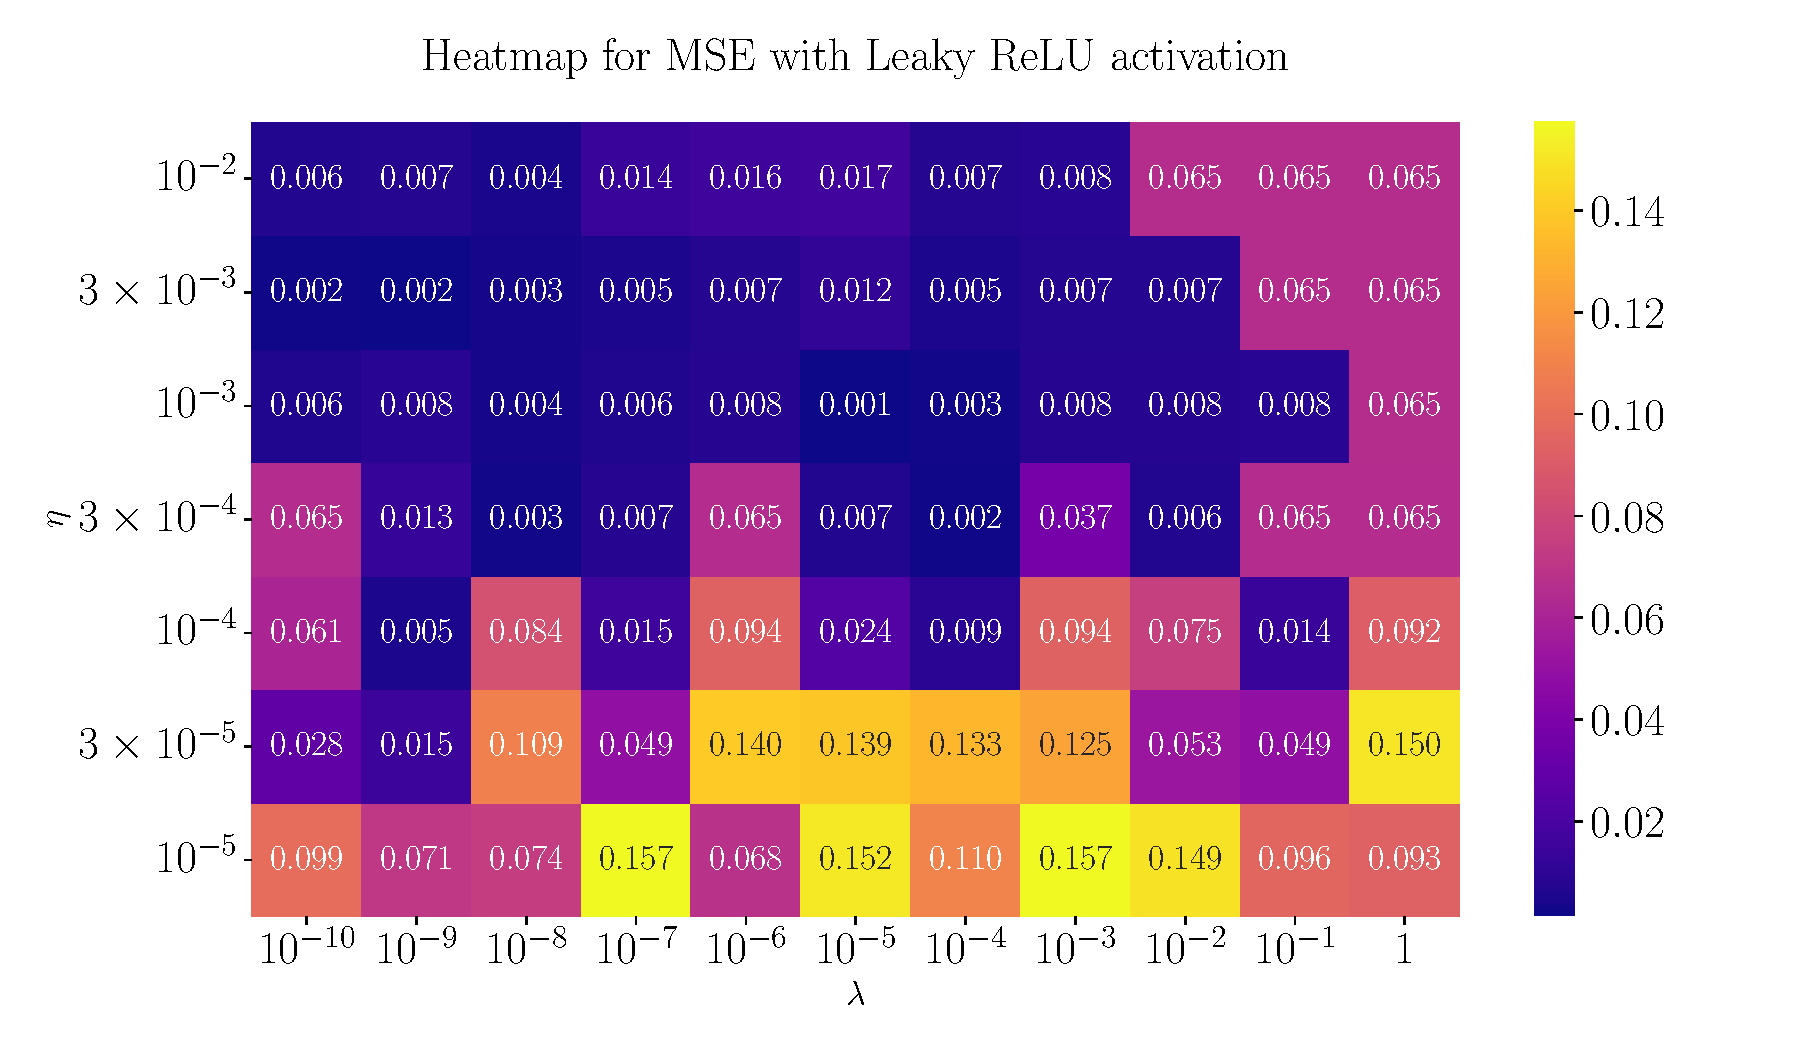
\includegraphics[width=\textwidth]{Figures/Heatmap_MSE_Leaky ReLU_Franke_Epochs250.pdf}
		\caption{LReLU}
	\end{subfigure}
	\hfill\newline
	\begin{subfigure}{0.41\textwidth}
		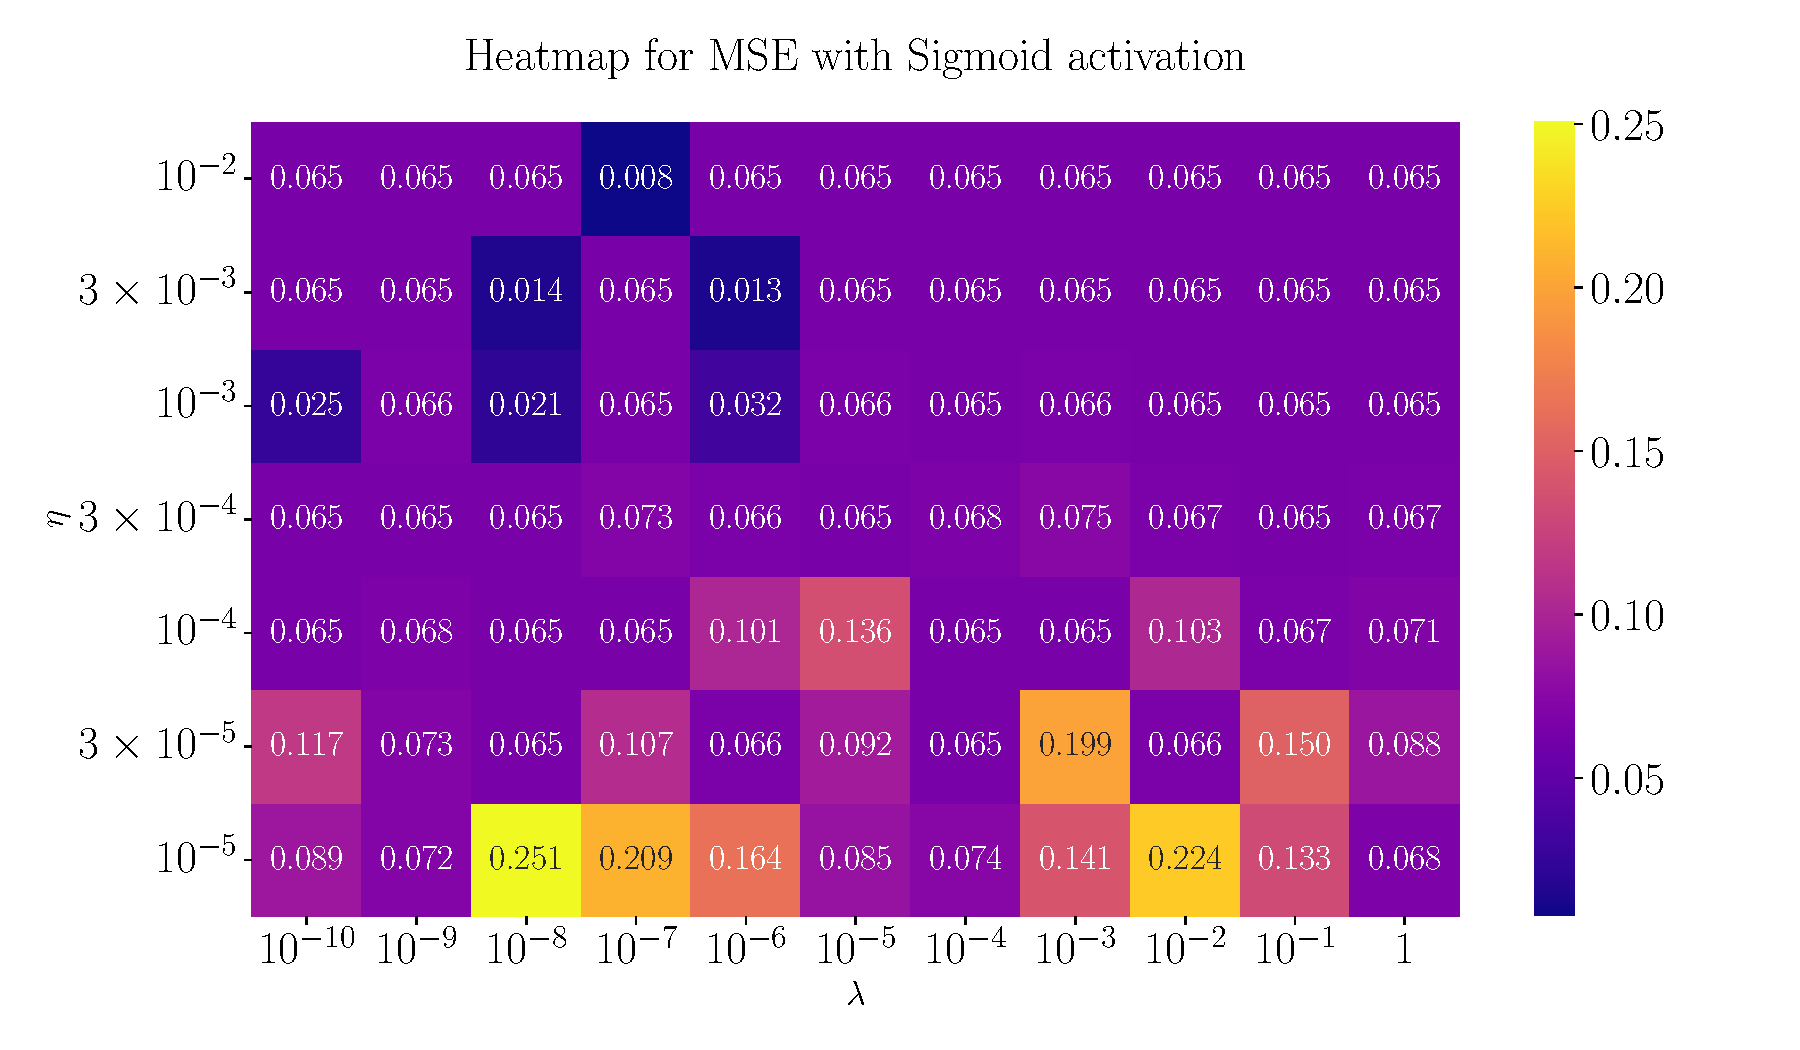
\includegraphics[width=\textwidth]{Figures/Heatmap_MSE_Sigmoid_Franke_Epochs250.pdf}
		\caption{Sigmoid}
	\end{subfigure}
	\caption{MSE for various combinations of $\eta$ and $\lambda$ for ReLU, LReLU and Sigmoid activation functions with $250$ epochs on the Franke function.}
	\label{fig:FFNN_Franke_heatmaps}	
\end{figure*}

%%%%%%%%% Logistic Regression %%%%%%%%%
\begin{figure*}
	\begin{subfigure}{0.41\textwidth}
		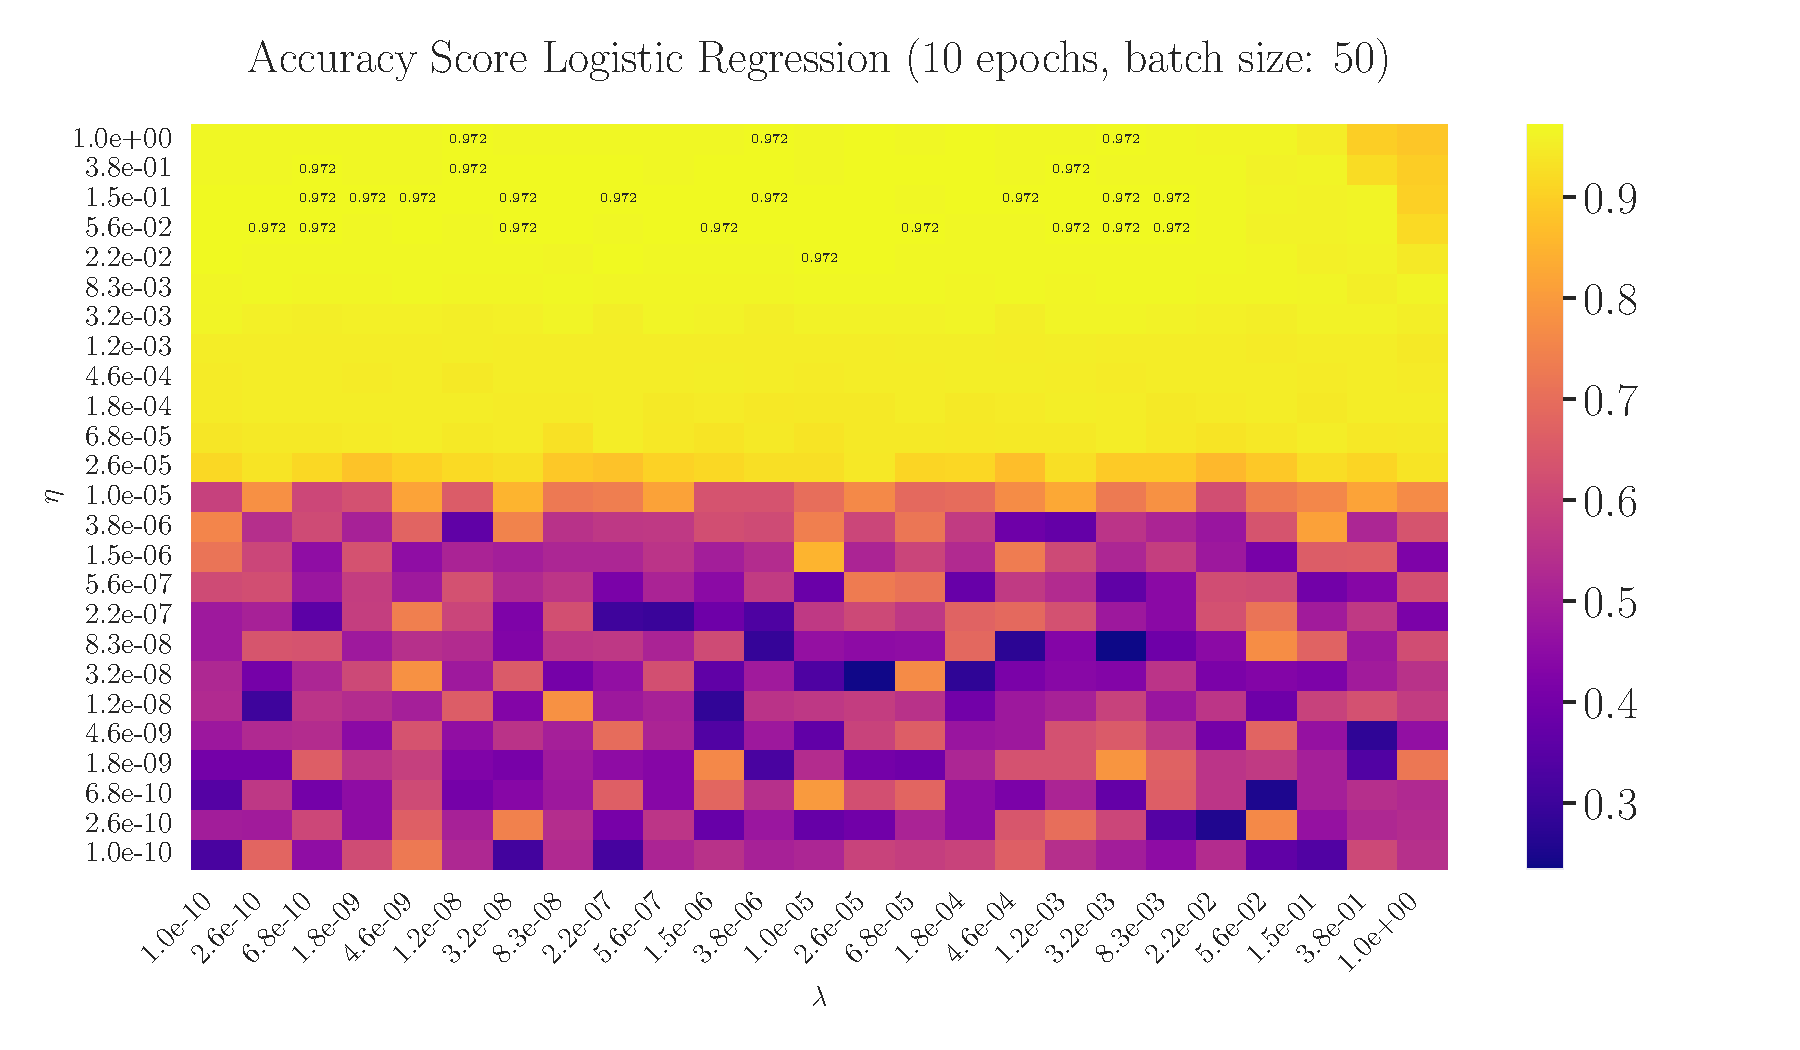
\includegraphics[width=\textwidth]{Figures/LogReg25x25_epoch10_batchS50.pdf}
		\label{fig:LogReg25x25_epoch10_bacthS50}
	\end{subfigure}
	\hfill
	\begin{subfigure}{0.41\textwidth}
		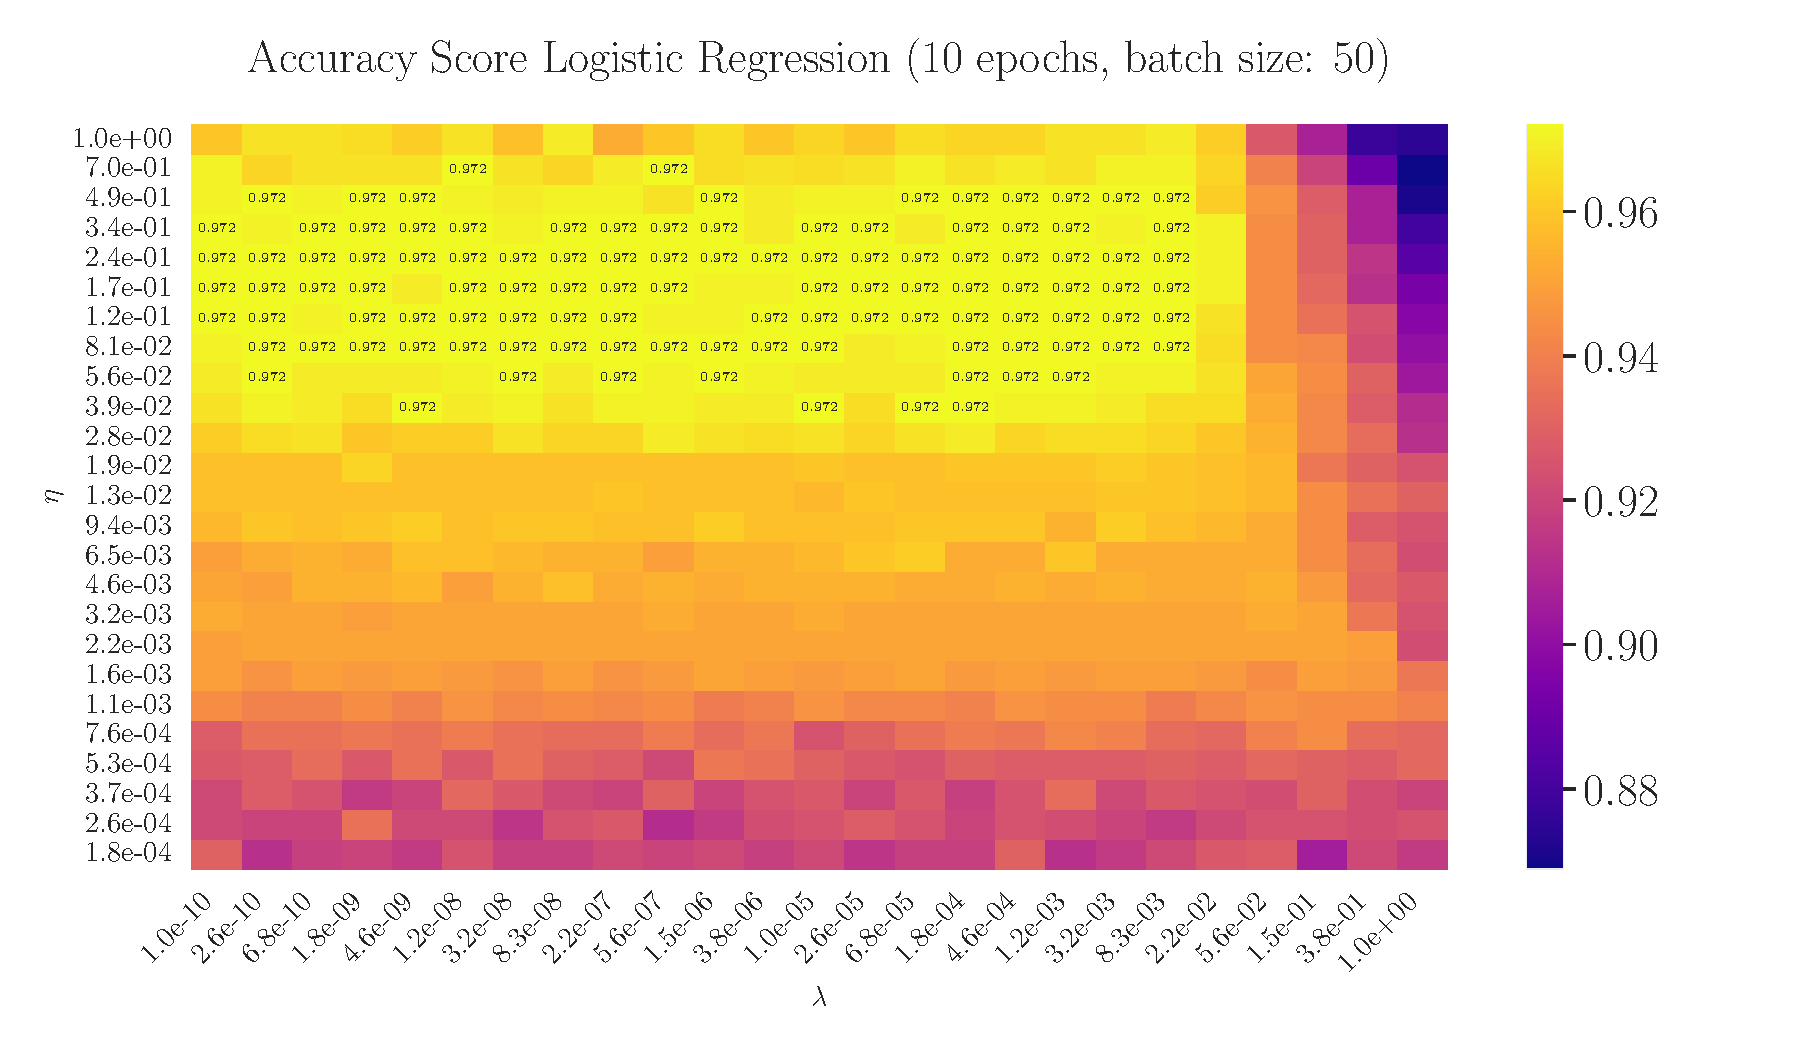
\includegraphics[width=\textwidth]{Figures/LogReg25x25_epoch10_batchS50_zoomed.pdf}
		\label{fig:LogReg25x25_epoch10_bacthS50_zoomed}
	\end{subfigure}
\hfill\newline
	\begin{subfigure}{0.41\textwidth}
		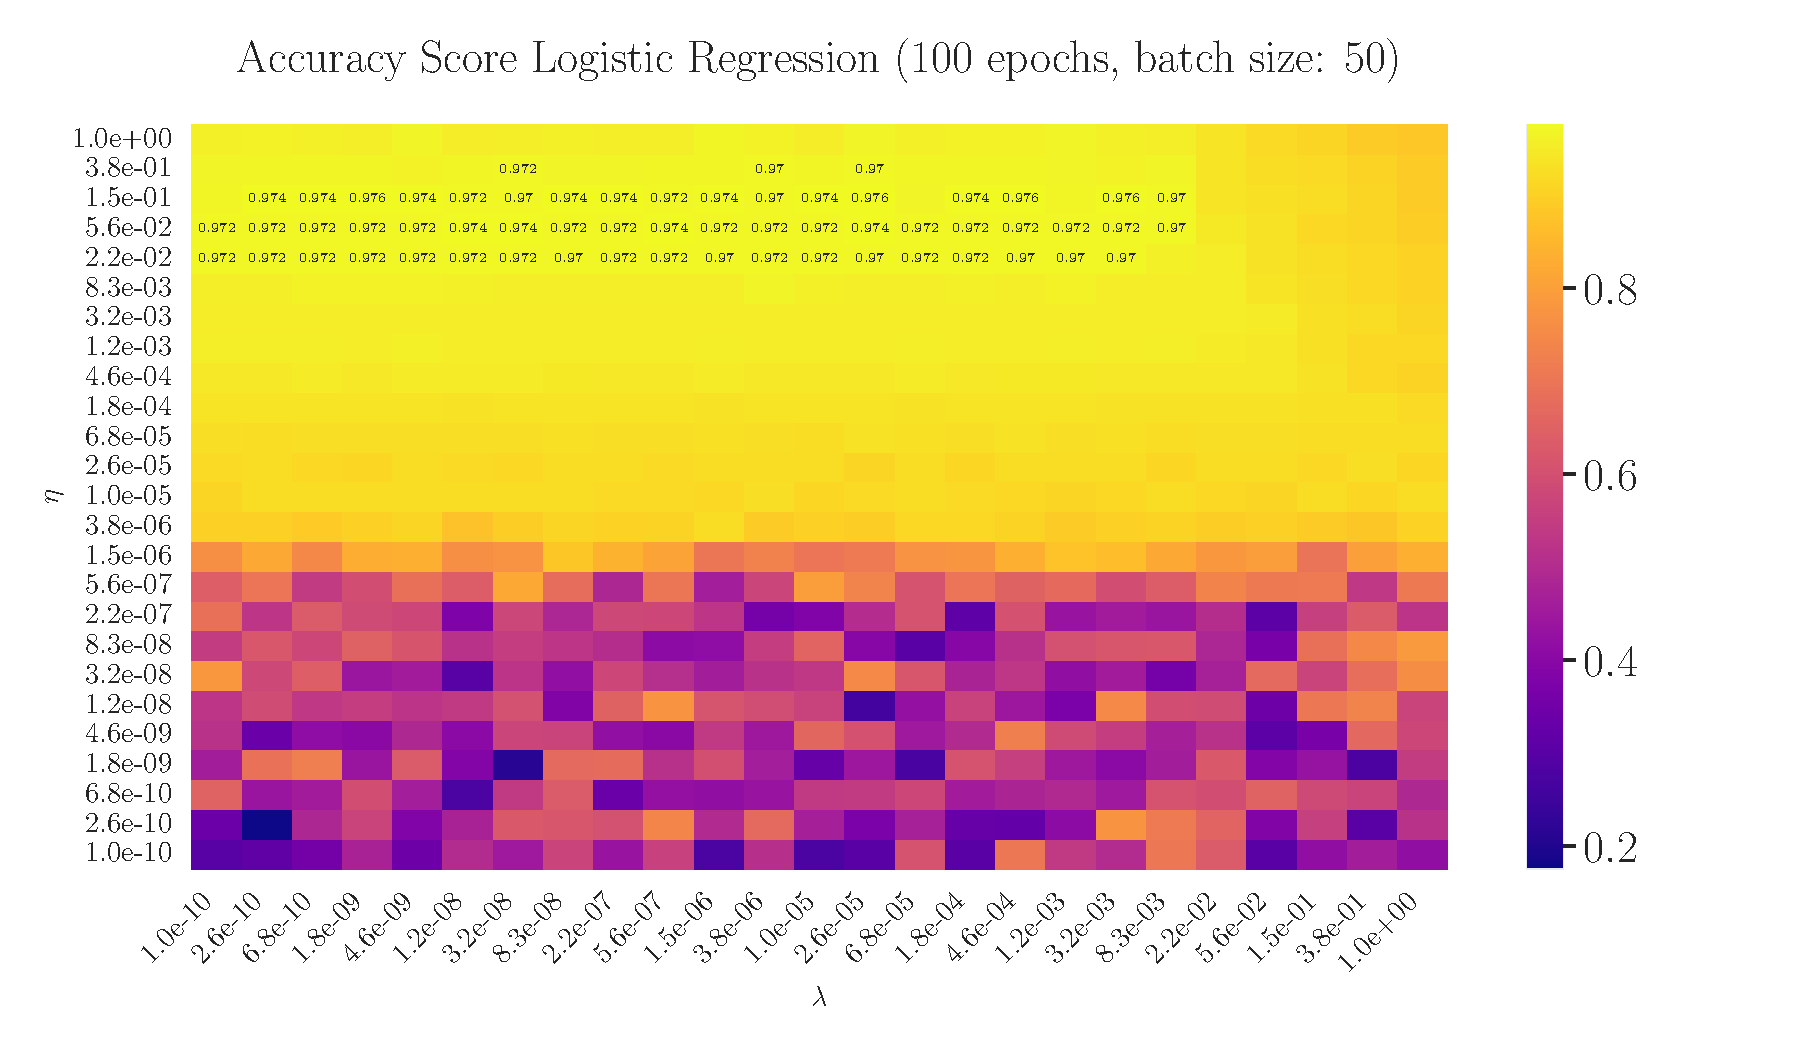
\includegraphics[width=\textwidth]{Figures/LogReg25x25_epoch100_batchS50.pdf}
		\label{fig:LogReg25x25_epoch100_bacthS50}
	\end{subfigure}
	\hfill
	\begin{subfigure}{0.41\textwidth}
		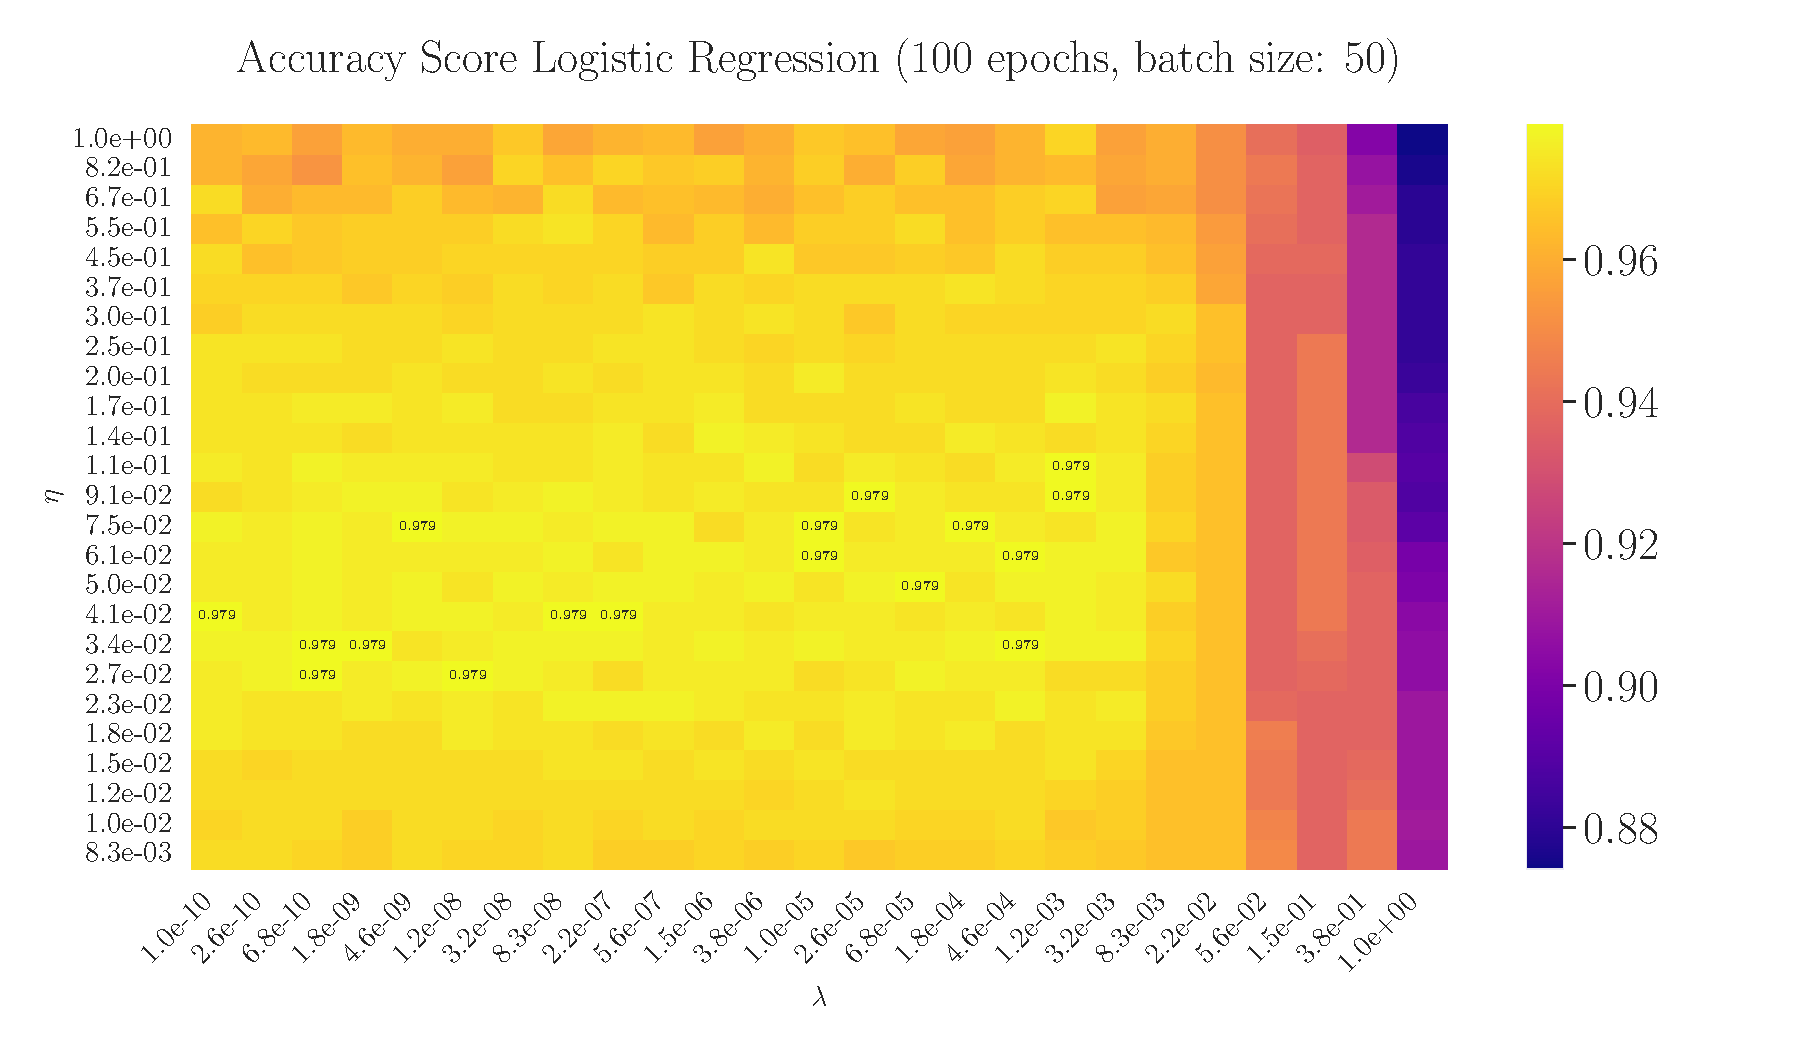
\includegraphics[width=\textwidth]{Figures/LogReg25x25_epoch100_batchS50_zoomed.pdf}
		\label{fig:LogReg25x25_epoch100_bacthS50_zoomed}
	\end{subfigure}
	\caption{Accuracy score for logistic regression, for number of epochs \(N=10\) (upper), \(N=100\) (lower). The figures to the right are zoomed in versions of the ones on the left. A varying learning rate has been used, with \(t_0=2\), \(t_{1} = 2/\eta_{\text{const}} \in [10^{-10}, 1]\)}
	\label{fig:LogReg}
\end{figure*}

\begin{figure*}[ht!]
	\begin{subfigure}{0.41\textwidth}
		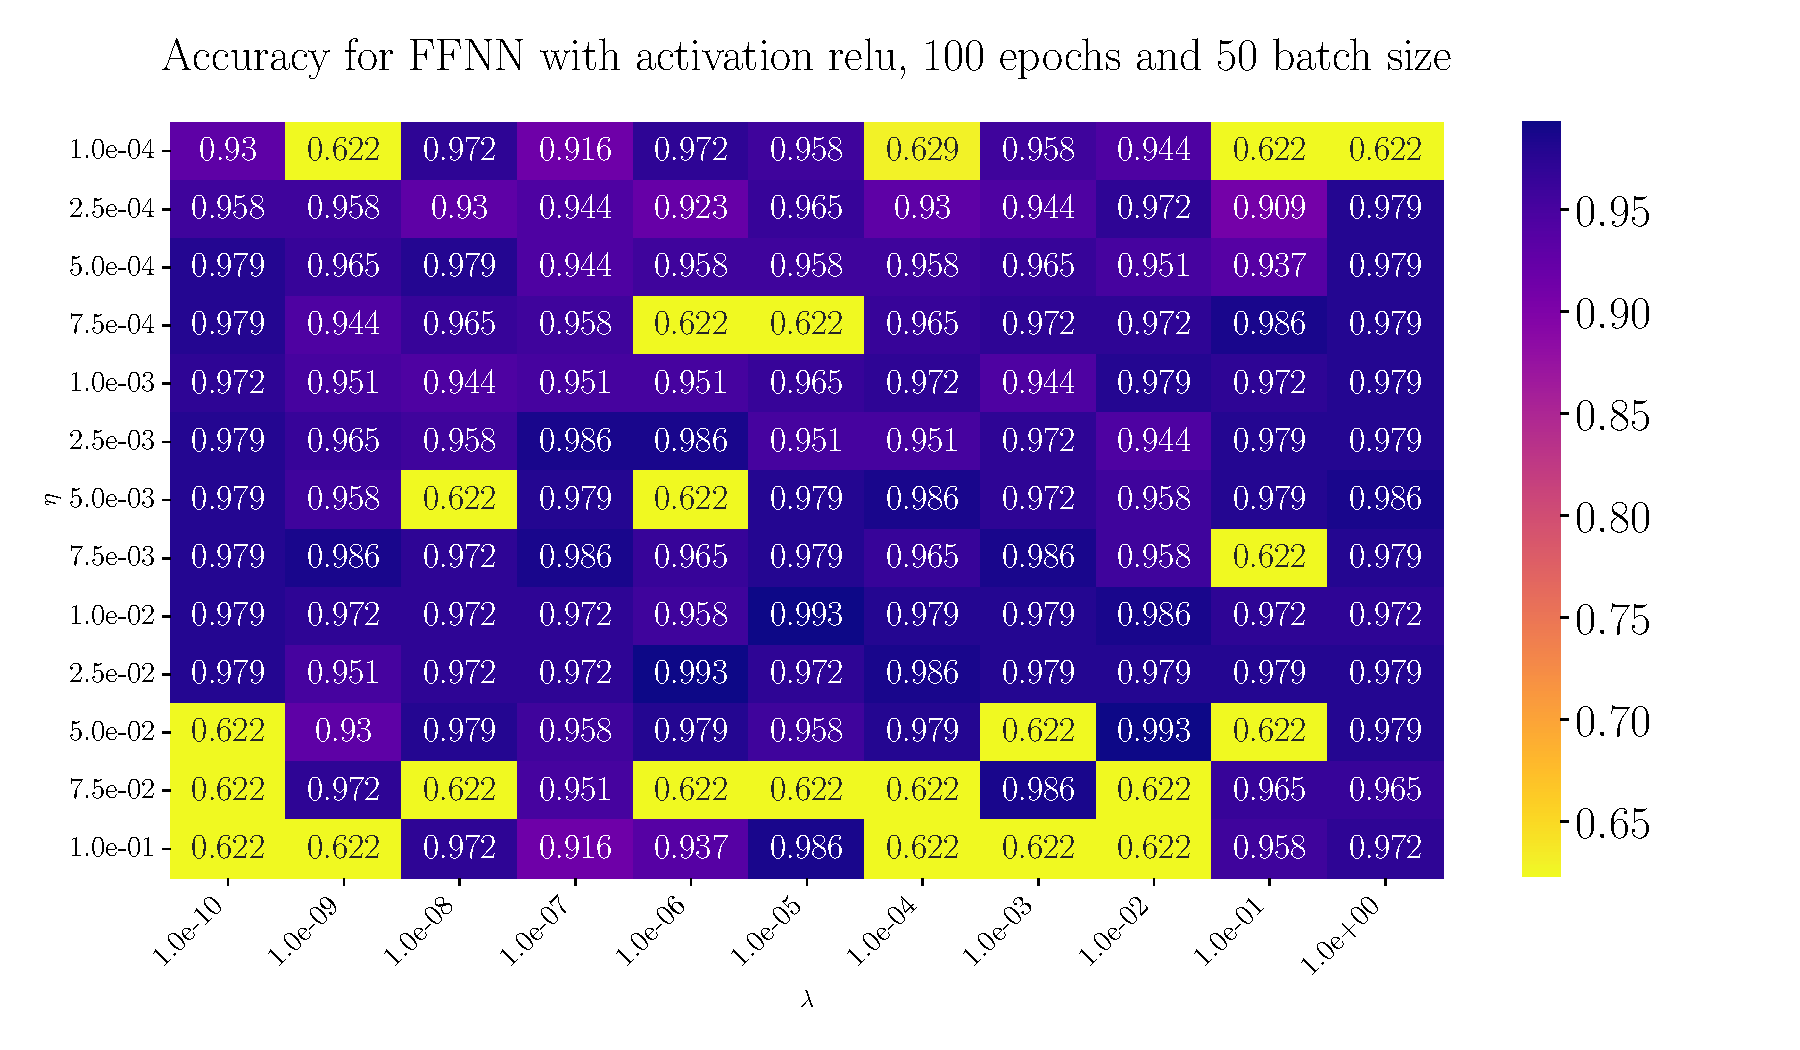
\includegraphics[width=\textwidth]{Figures/Cancer_Accuracy_Heatmap_relu_Epochs100.pdf}
		\caption{ReLU}
		\label{fig:ReLU_heatmap}
	\end{subfigure}
	\hfill
	\begin{subfigure}{0.41\textwidth}
		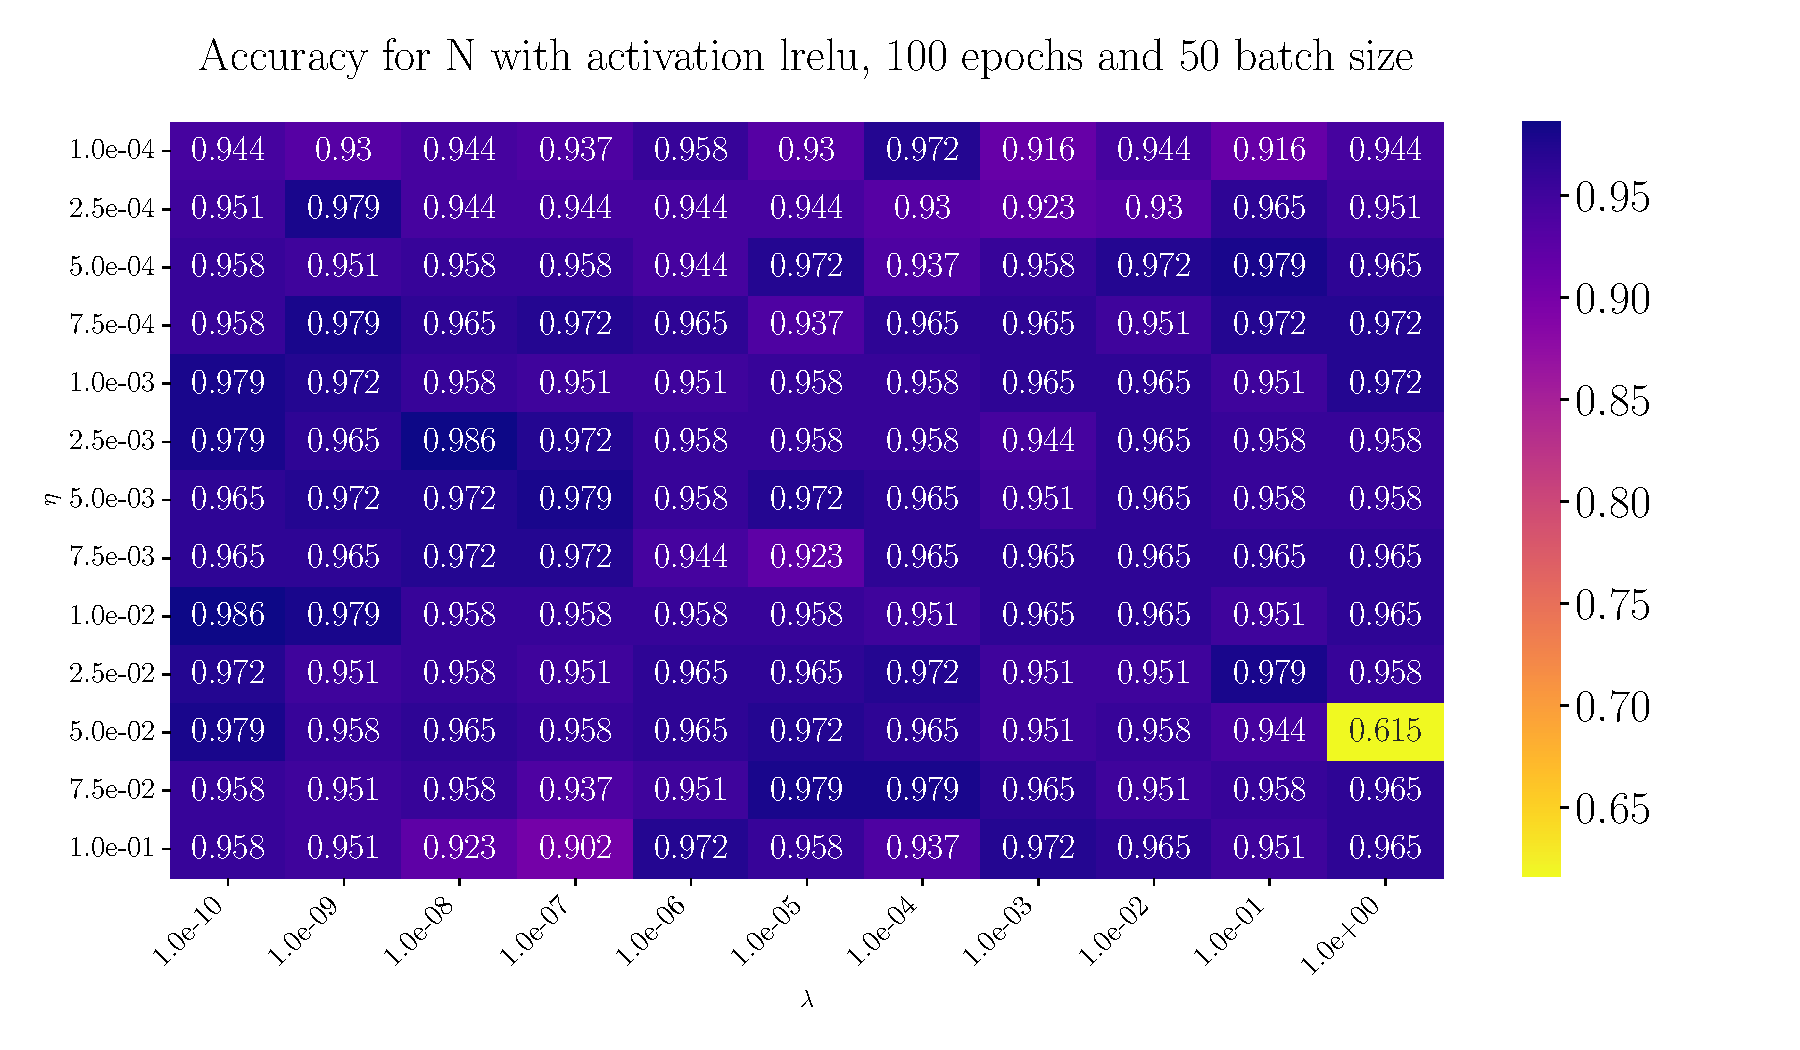
\includegraphics[width=\textwidth]{Figures/Cancer_Accuracy_Heatmap_lrelu_Epochs100.pdf}
		\caption{LReLU}
		\label{fig:LReLU_heatmap}
	\end{subfigure}
	\hfill\newline
	\begin{subfigure}{0.41\textwidth}
		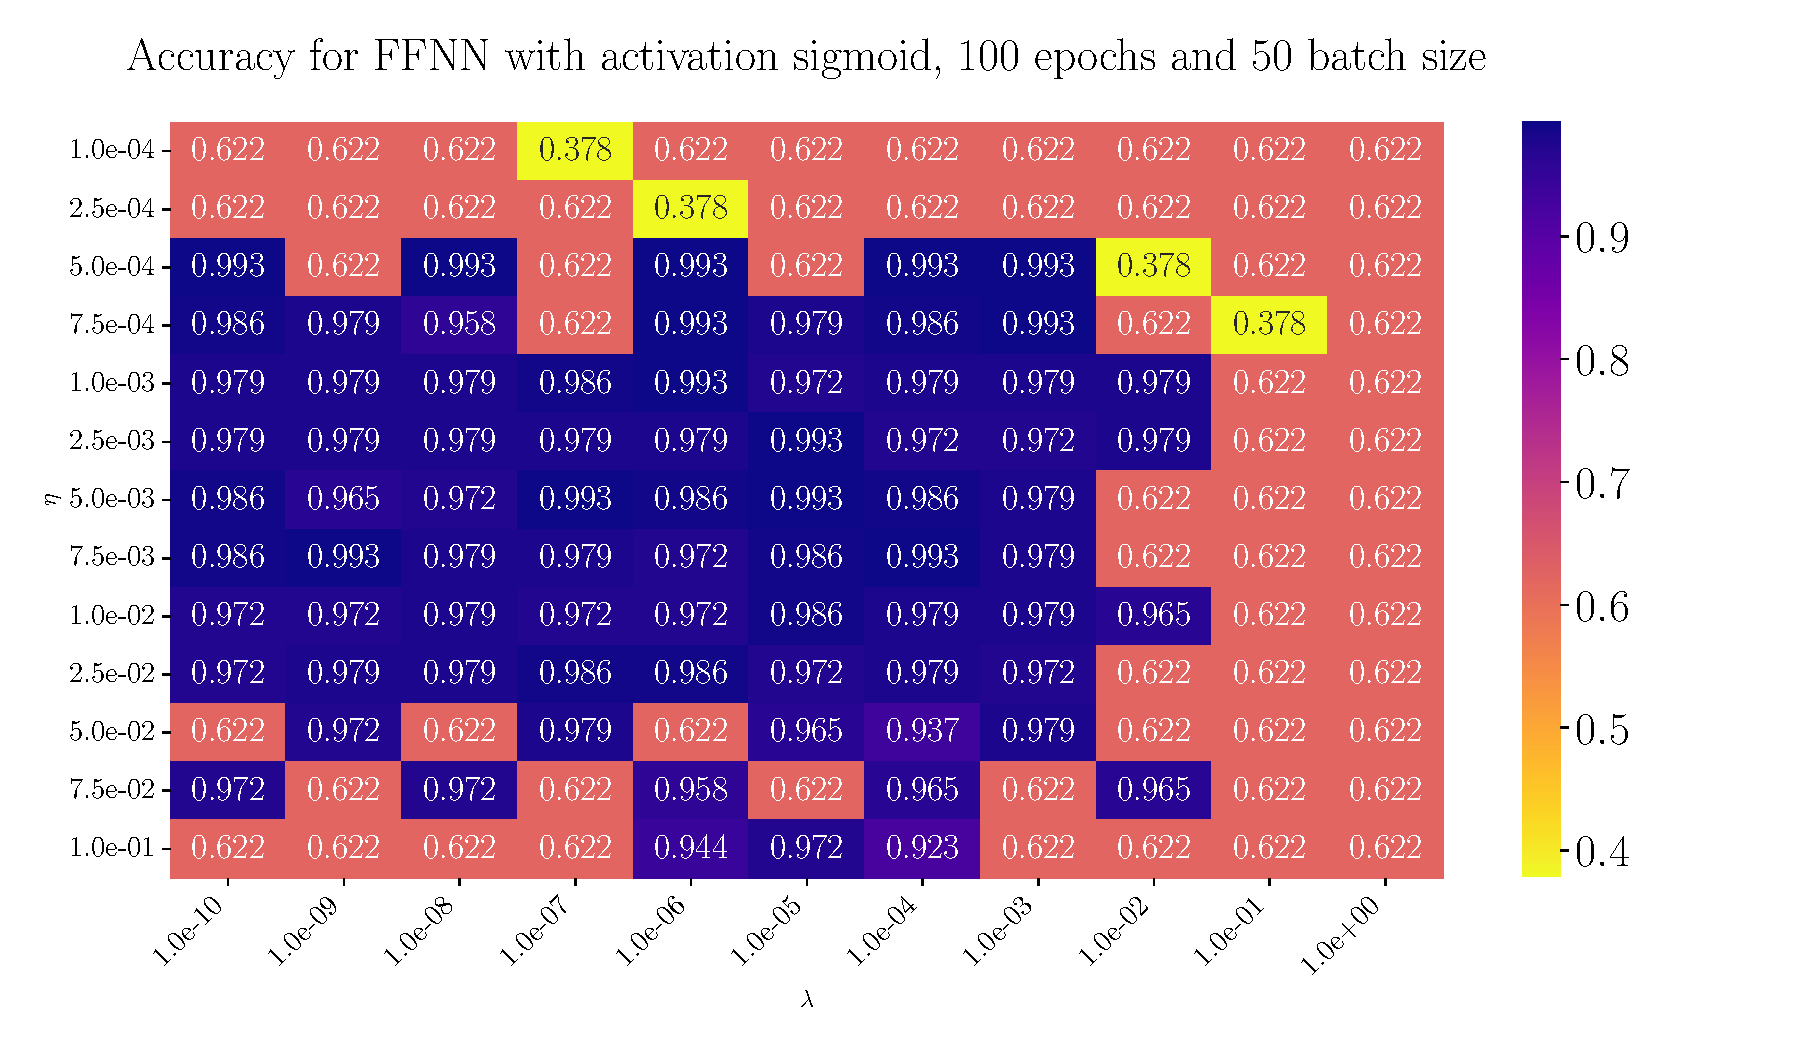
\includegraphics[width=\textwidth]{Figures/Cancer_Accuracy_Heatmap_sigmoid_Epochs100.pdf}
		\caption{Sigmoid}
		\label{fig:Sigmoid_heatmap}
	\end{subfigure}
	\caption{Accuracy for various combinations of $\eta$ and $\lambda$ for ReLU, LReLU and Sigmoid activation functions with $100$ epochs and $50$ batch size on the breast cancer dataset.}
	\label{fig:FFNN_cancer_heatmaps}
\end{figure*}

%%%%%%%%%%%%%%%% Bunch of different MSE plots, linear regression %%%%%%%%%%%%%%%%

% % plainSGD with varying learning rate
% \begin{figure*}
% 	\begin{subfigure}{0.41\textwidth}
% 		\includegraphics[width=\textwidth]{Figures/LinRegplainSGD_varyEta_10epochs_5batchS.pdf}
% 		\caption{\(10\) epochs and a batch size of \(5\).}
% 		\label{fig:LinRegplainSGD_varyEta_10epochs_5batchS}
% 	\end{subfigure}
% 	\hfill
% 	\begin{subfigure}{0.41\textwidth}
% 		\includegraphics[width=\textwidth]{Figures/LinRegplainSGD_varyEta_100epochs_5batchS.pdf}
% 		\caption{\(100\) epochs and a batch size of \(5\).}
% 		\label{fig:LinRegplainSGD_varyEta_100epochs_5batchS}
% 	\end{subfigure}
% \hfill\newline
% \begin{subfigure}{0.41\textwidth}
% 	\includegraphics[width=\textwidth]{Figures/LinRegplainSGD_varyEta_10epochs_10batchS.pdf}
% 	\caption{\(10\) epochs and a batch size of \(10\).}
% 	\label{fig:LinRegplainSGD_varyEta_10epochs_5batchS}
% \end{subfigure}
% \hfill
% \begin{subfigure}{0.41\textwidth}
% 	\includegraphics[width=\textwidth]{Figures/LinRegplainSGD_varyEta_100epochs_10batchS.pdf}
% 	\caption{\(100\) epochs and a batch size of \(10\).}
% 	\label{fig:LinRegplainSGD_varyEta_100epochs_5batchS}
% \end{subfigure}
% \caption{MSE scores using plain SGD with a varying learning rate; see \eqref{eq:varyin_learning_rate}, \(t_0=2\) and \(t_1=\eta\), where \(\eta\) can be read from the y-axis.}
% \label{fig:PlangeSGD_varyEta}
% \end{figure*}

% % plainSGD with constant learning rate
% \begin{figure*}
% 	\begin{subfigure}{0.41\textwidth}
% 		\includegraphics[width=\textwidth]{Figures/LinRegplainSGD_constEta_10epochs_5batchS.pdf}
% 		\caption{\(10\) epochs and a batch size of \(5\).}
% 		\label{fig:LinRegplainSGD_constEta_10epochs_5batchS}
% 	\end{subfigure}
% 	\hfill
% 	\begin{subfigure}{0.41\textwidth}
% 		\includegraphics[width=\textwidth]{Figures/LinRegplainSGD_constEta_100epochs_batchS10.pdf}
% 		\caption{\(100\) epochs and a batch size of \(5\).}
% 		\label{fig:LinRegplainSGD_constEta_100epochs_5batchS}
% 	\end{subfigure}
% \hfill\newline
% \begin{subfigure}{0.41\textwidth}
% 	\includegraphics[width=\textwidth]{Figures/LinRegplainSGD_constEta_10epochs_10batchS.pdf}
% 	\caption{\(10\) epochs and a batch size of \(10\).}
% 	\label{fig:LinRegplainSGD_constEta_10epochs_5batchS}
% \end{subfigure}
% \hfill
% \begin{subfigure}{0.41\textwidth}
% 	\includegraphics[width=\textwidth]{Figures/LinRegplainSGD_constEta_100epochs_batchS10.pdf}
% 	\caption{\(100\) epochs and a batch size of \(10\).}
% 	\label{fig:LinRegplainSGD_constEta_100epochs_5batchS}
% \end{subfigure}
% \caption{MSE scores using plain SGD with a constant learning rate.}
% \label{fig:PlangeSGD_constEta}
% \end{figure*}


% % RMSprop with varying learning rate
% \begin{figure*}
% 	\begin{subfigure}{0.41\textwidth}
% 		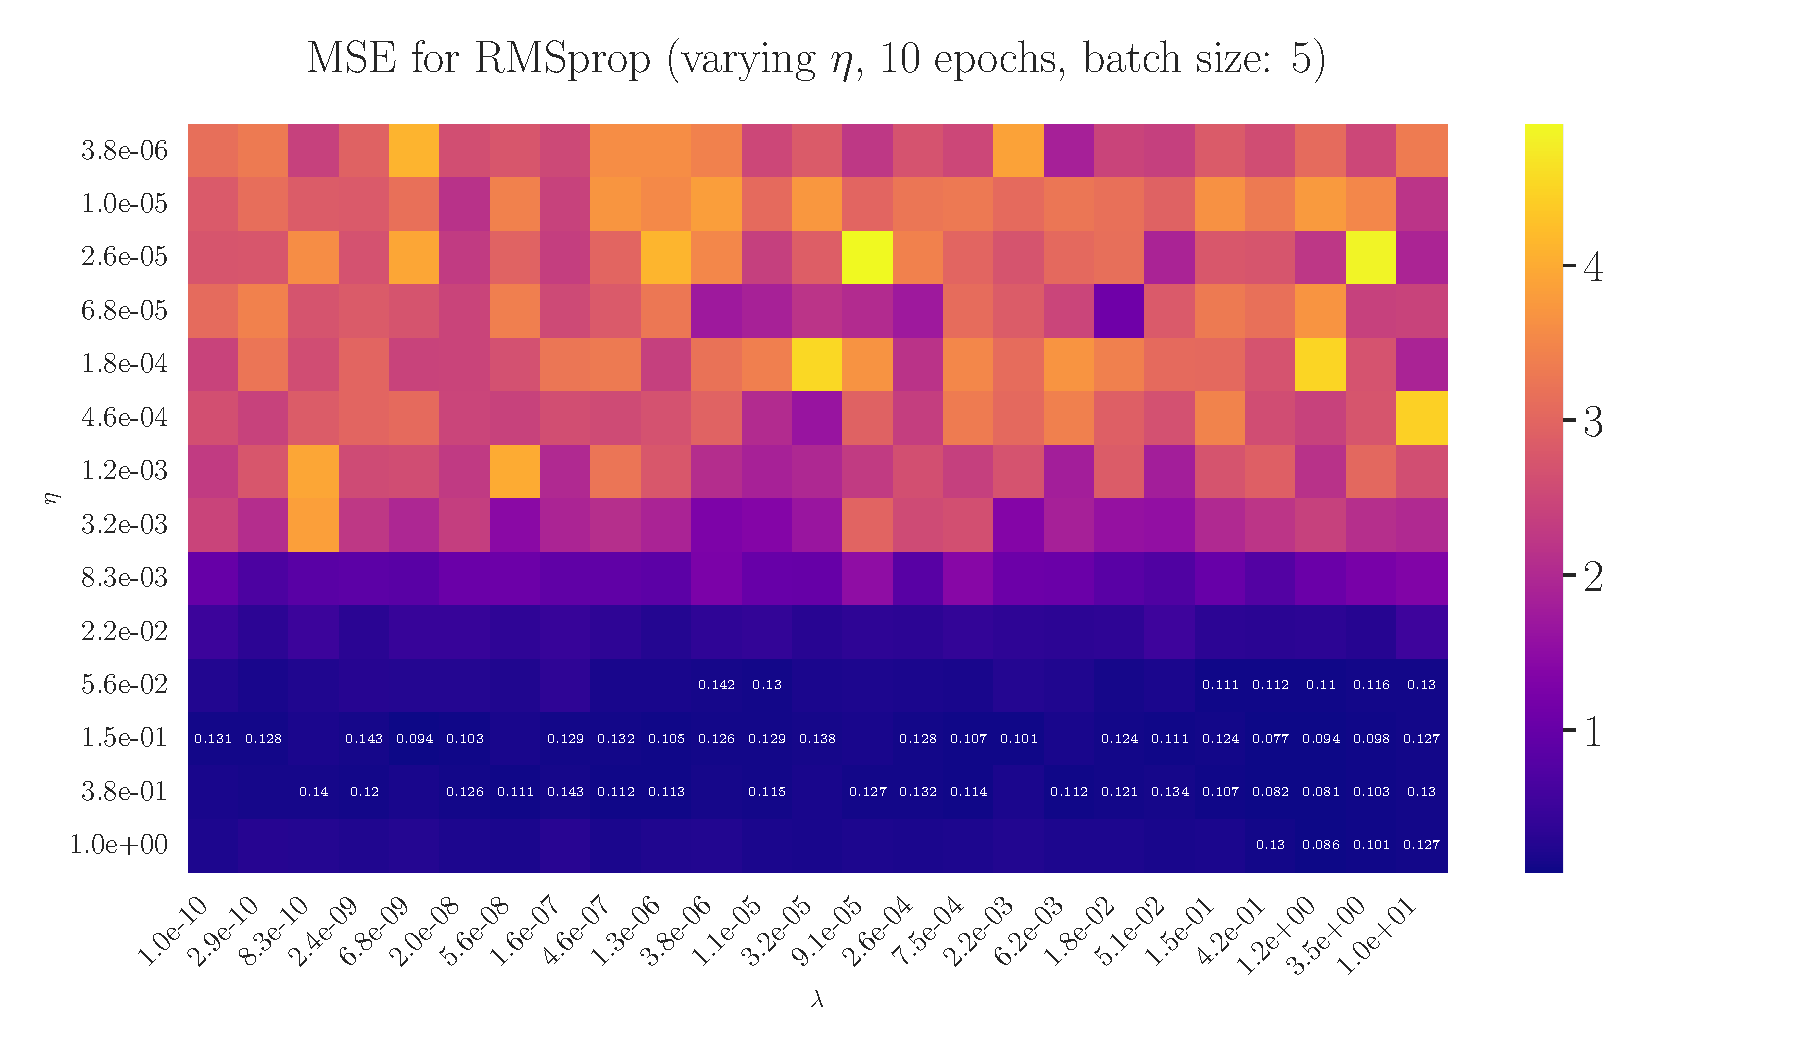
\includegraphics[width=\textwidth]{Figures/LinRegRMSprop_varyEta_10epochs_batchS5.pdf}
% 		\caption{\(10\) epochs and a batch size of \(5\).}
% 		\label{fig:LinRegRMSprop_varyEta_10epochs_5batchS}
% 	\end{subfigure}
% 	\hfill
% 	\begin{subfigure}{0.41\textwidth}
% 		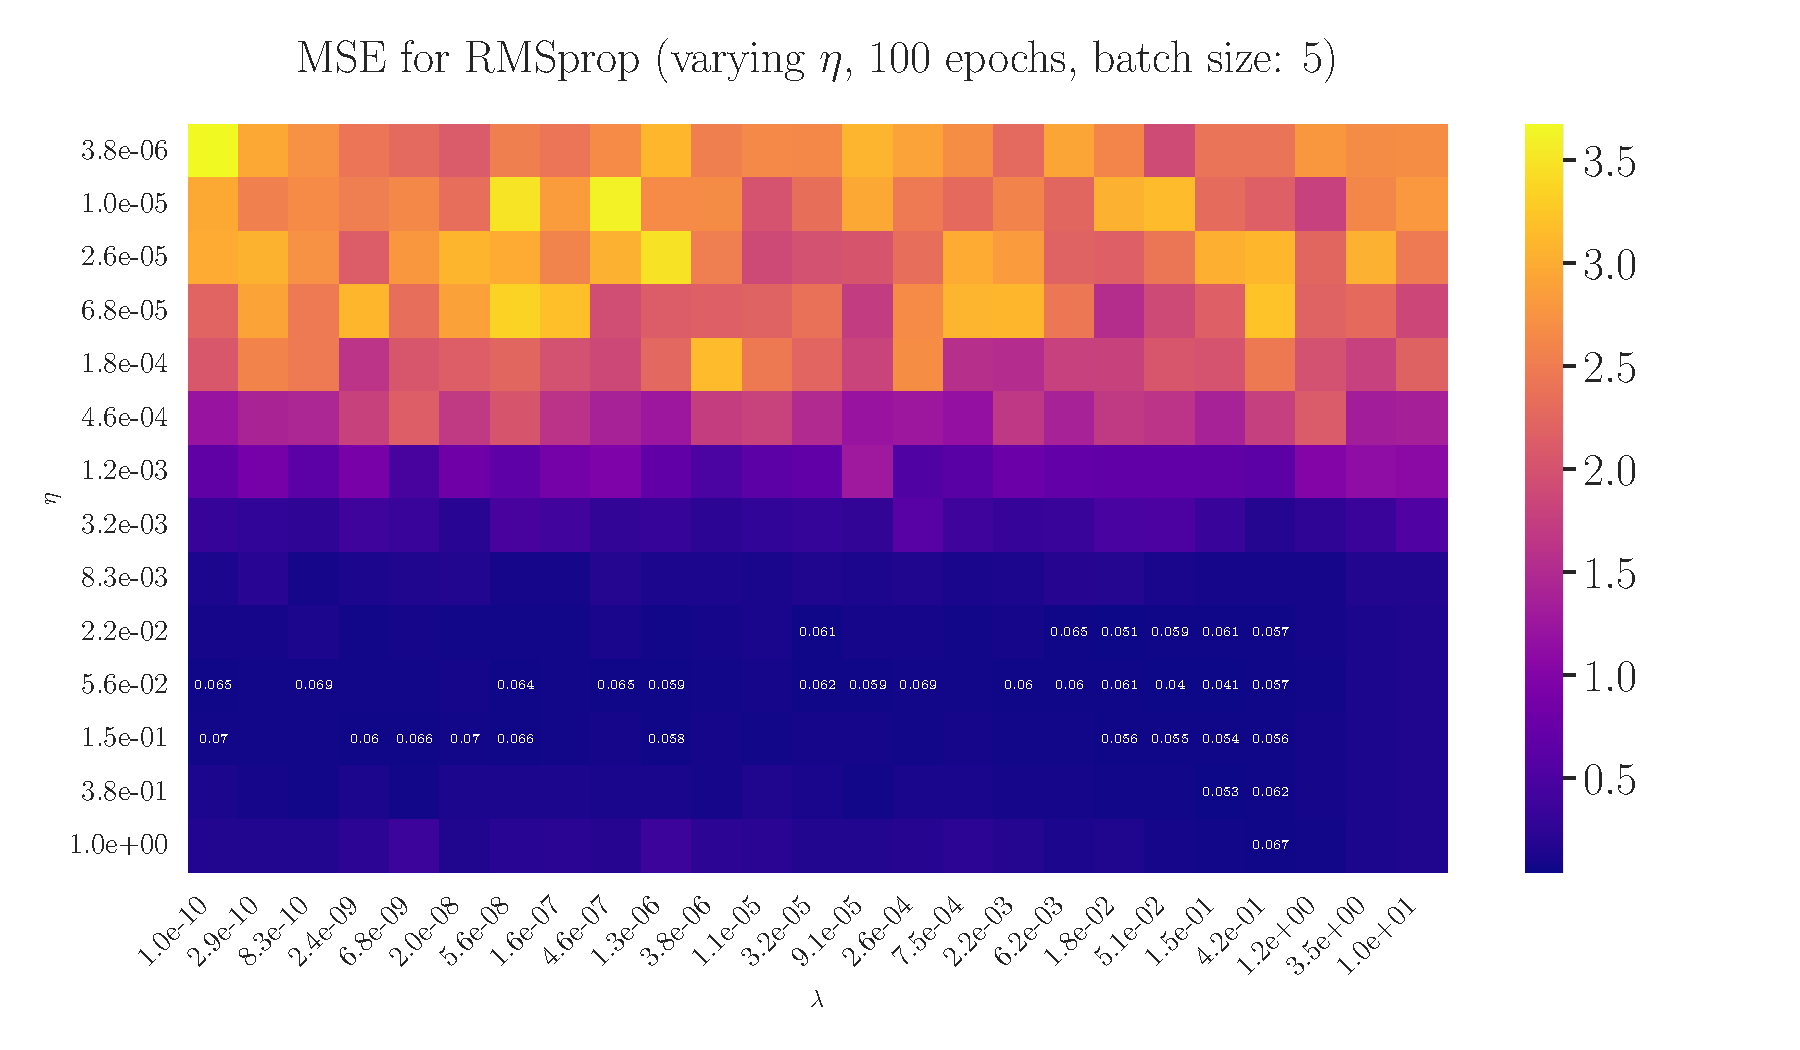
\includegraphics[width=\textwidth]{Figures/LinRegRMSprop_varyEta_100epochs_batchS5.pdf}
% 		\caption{\(100\) epochs and a batch size of \(5\).}
% 		\label{fig:LinRegRMSprop_varyEta_100epochs_5batchS}
% 	\end{subfigure}
% \hfill\newline
% \begin{subfigure}{0.41\textwidth}
% 	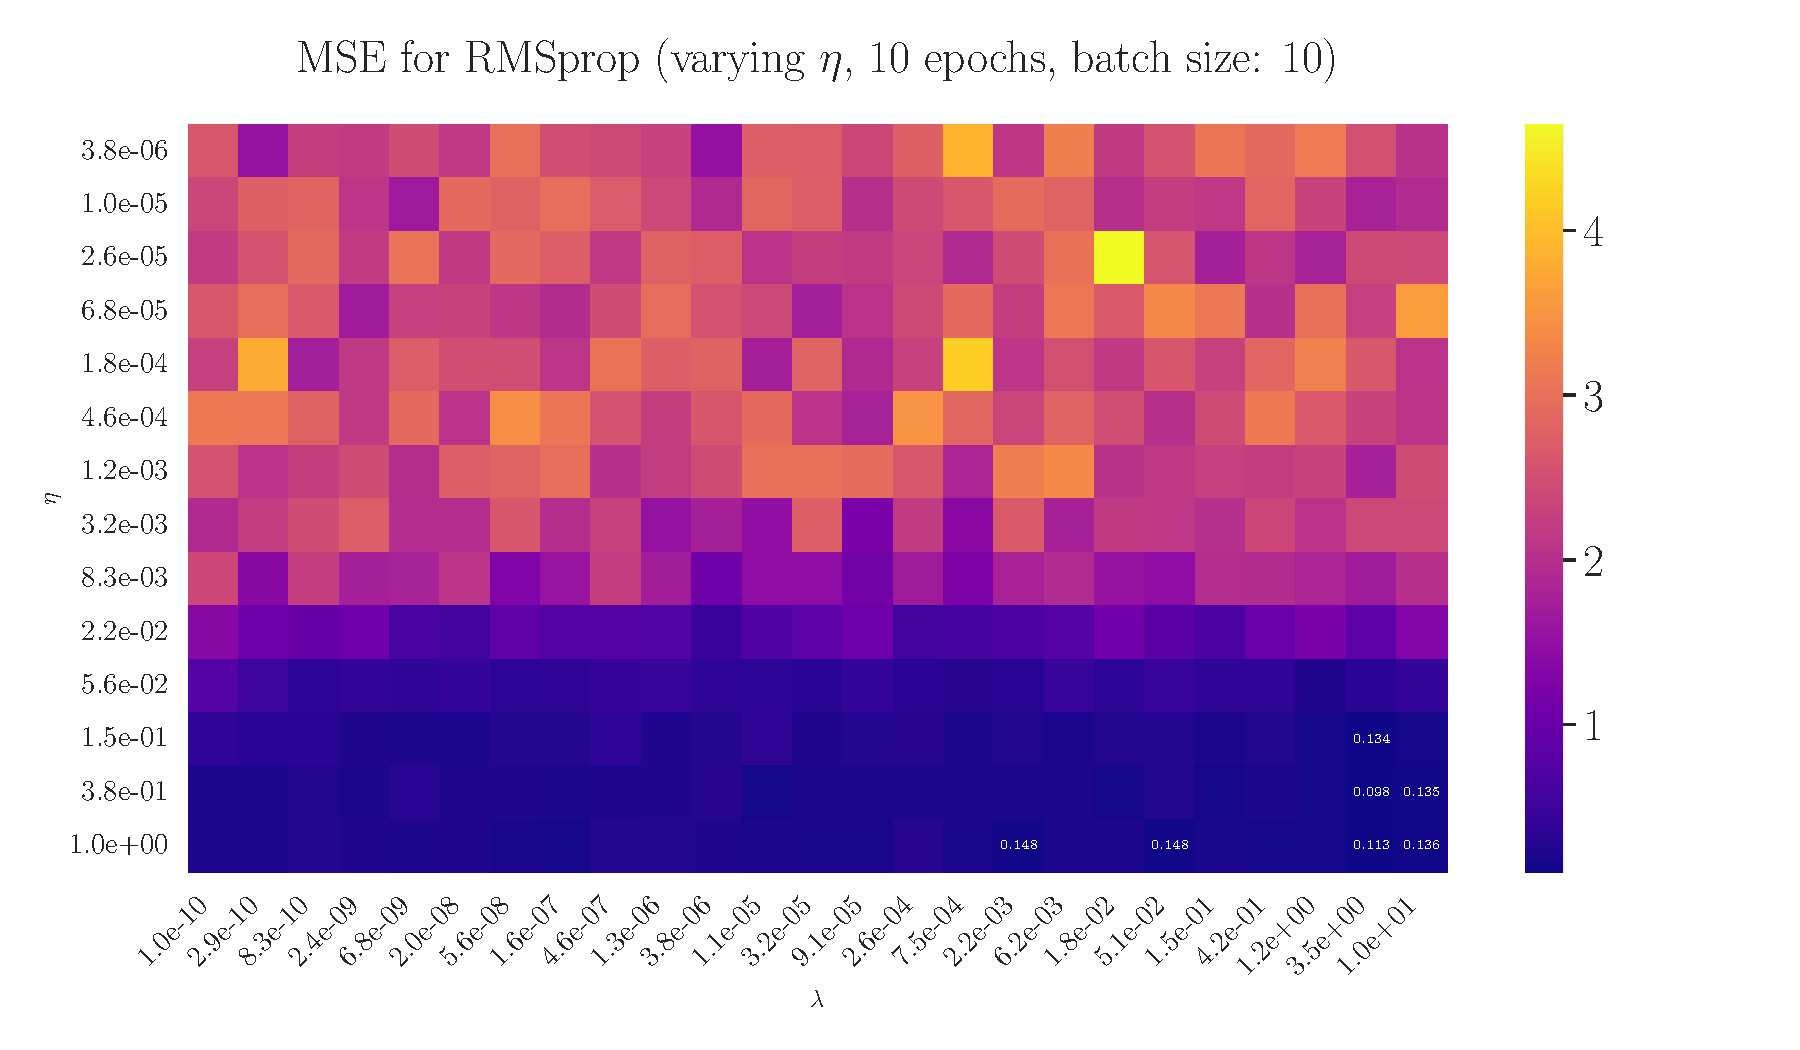
\includegraphics[width=\textwidth]{Figures/LinRegRMSprop_varyEta_10epochs_batchS10.pdf}
% 	\caption{\(10\) epochs and a batch size of \(10\).}
% 	\label{fig:LinRegRMSprop_varyEta_10epochs_5batchS}
% \end{subfigure}
% \hfill
% \begin{subfigure}{0.41\textwidth}
% 	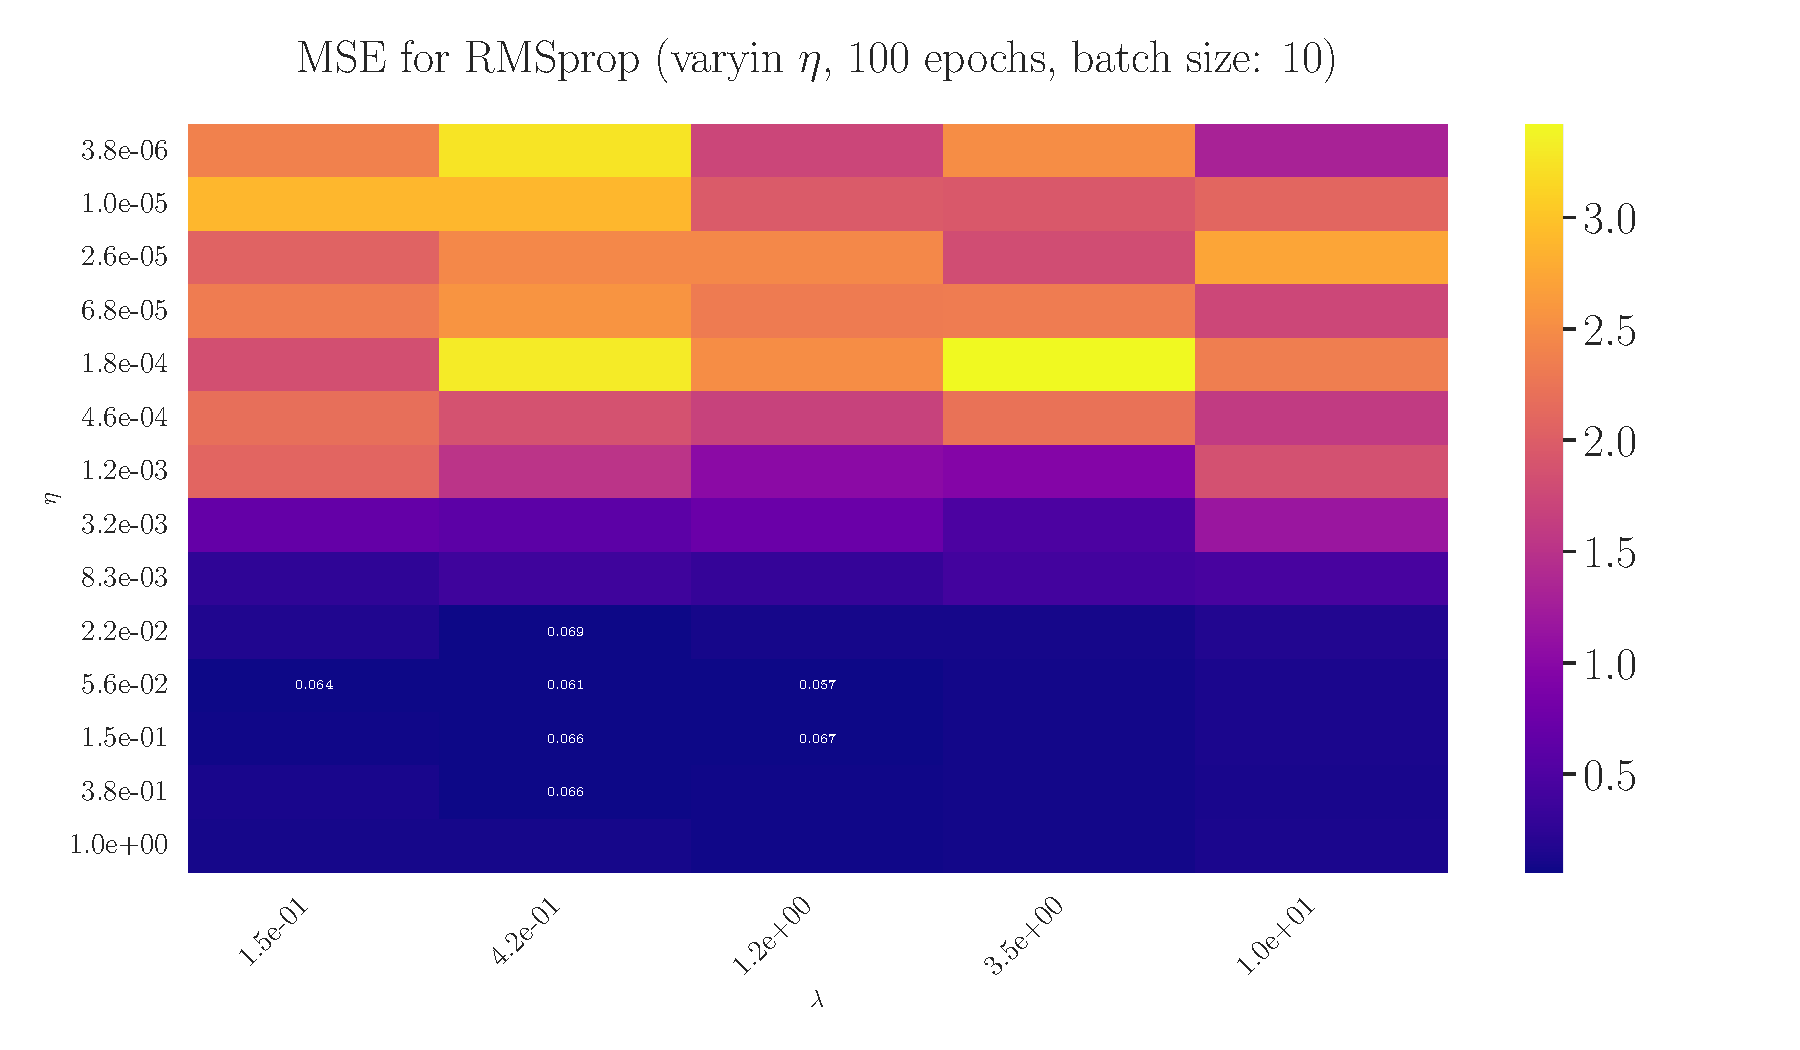
\includegraphics[width=\textwidth]{Figures/LinRegRMSprop_varyEta_100epochs_batchS10.pdf}
% 	\caption{\(100\) epochs and a batch size of \(10\).}
% 	\label{fig:LinRegRMSprop_varyEta_100epochs_5batchS}
% \end{subfigure}
% \caption{MSE scores using RMSprop with a varying learning rate; see \eqref{eq:varyin_learning_rate}, \(t_0=2\) and \(t_1=\eta\), where \(\eta\) can be read from the y-axis.}
% \label{fig:RMSprop_varyEta}
% \end{figure*}

% % RMSprop with constant learning rate
% \begin{figure*}
% 	\begin{subfigure}{0.41\textwidth}
% 		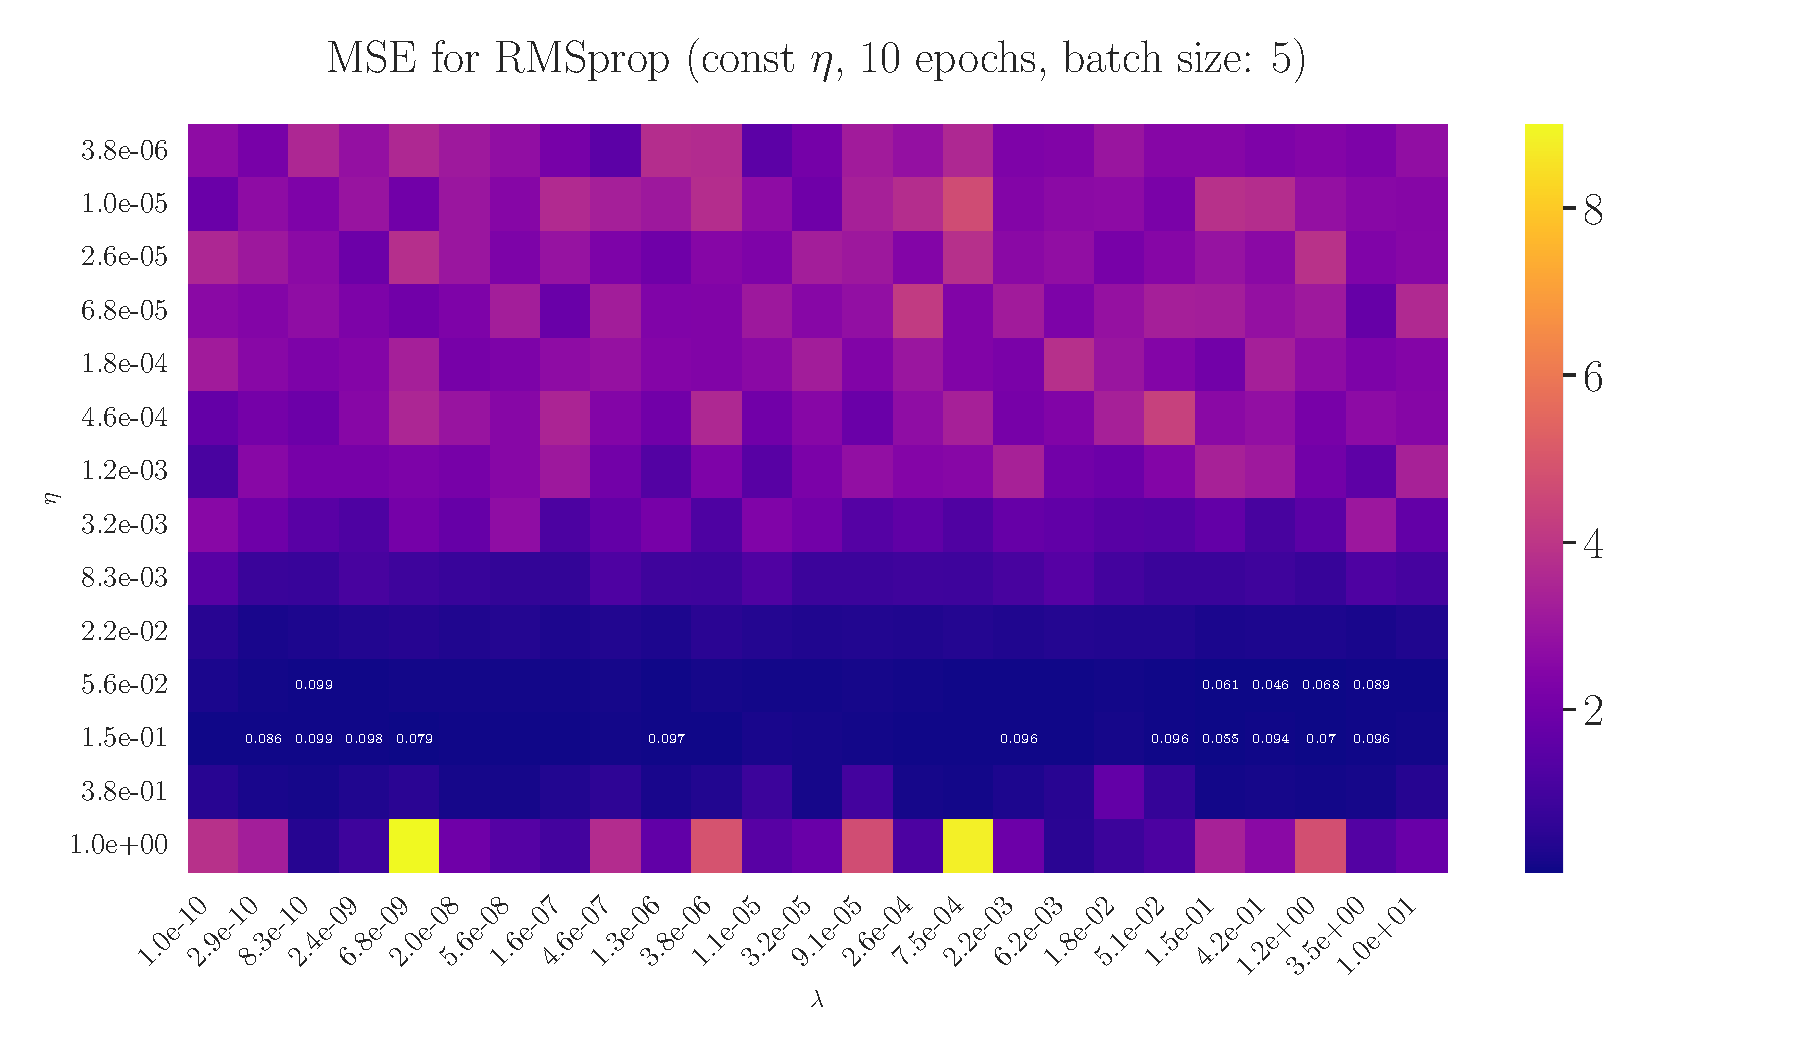
\includegraphics[width=\textwidth]{Figures/LinRegRMSprop_constEta_10epochs_batchS5.pdf}
% 		\caption{\(10\) epochs and a batch size of \(5\).}
% 		\label{fig:LinRegRMSprop_constEta_10epochs_5batchS}
% 	\end{subfigure}
% 	\hfill
% 	\begin{subfigure}{0.41\textwidth}
% 		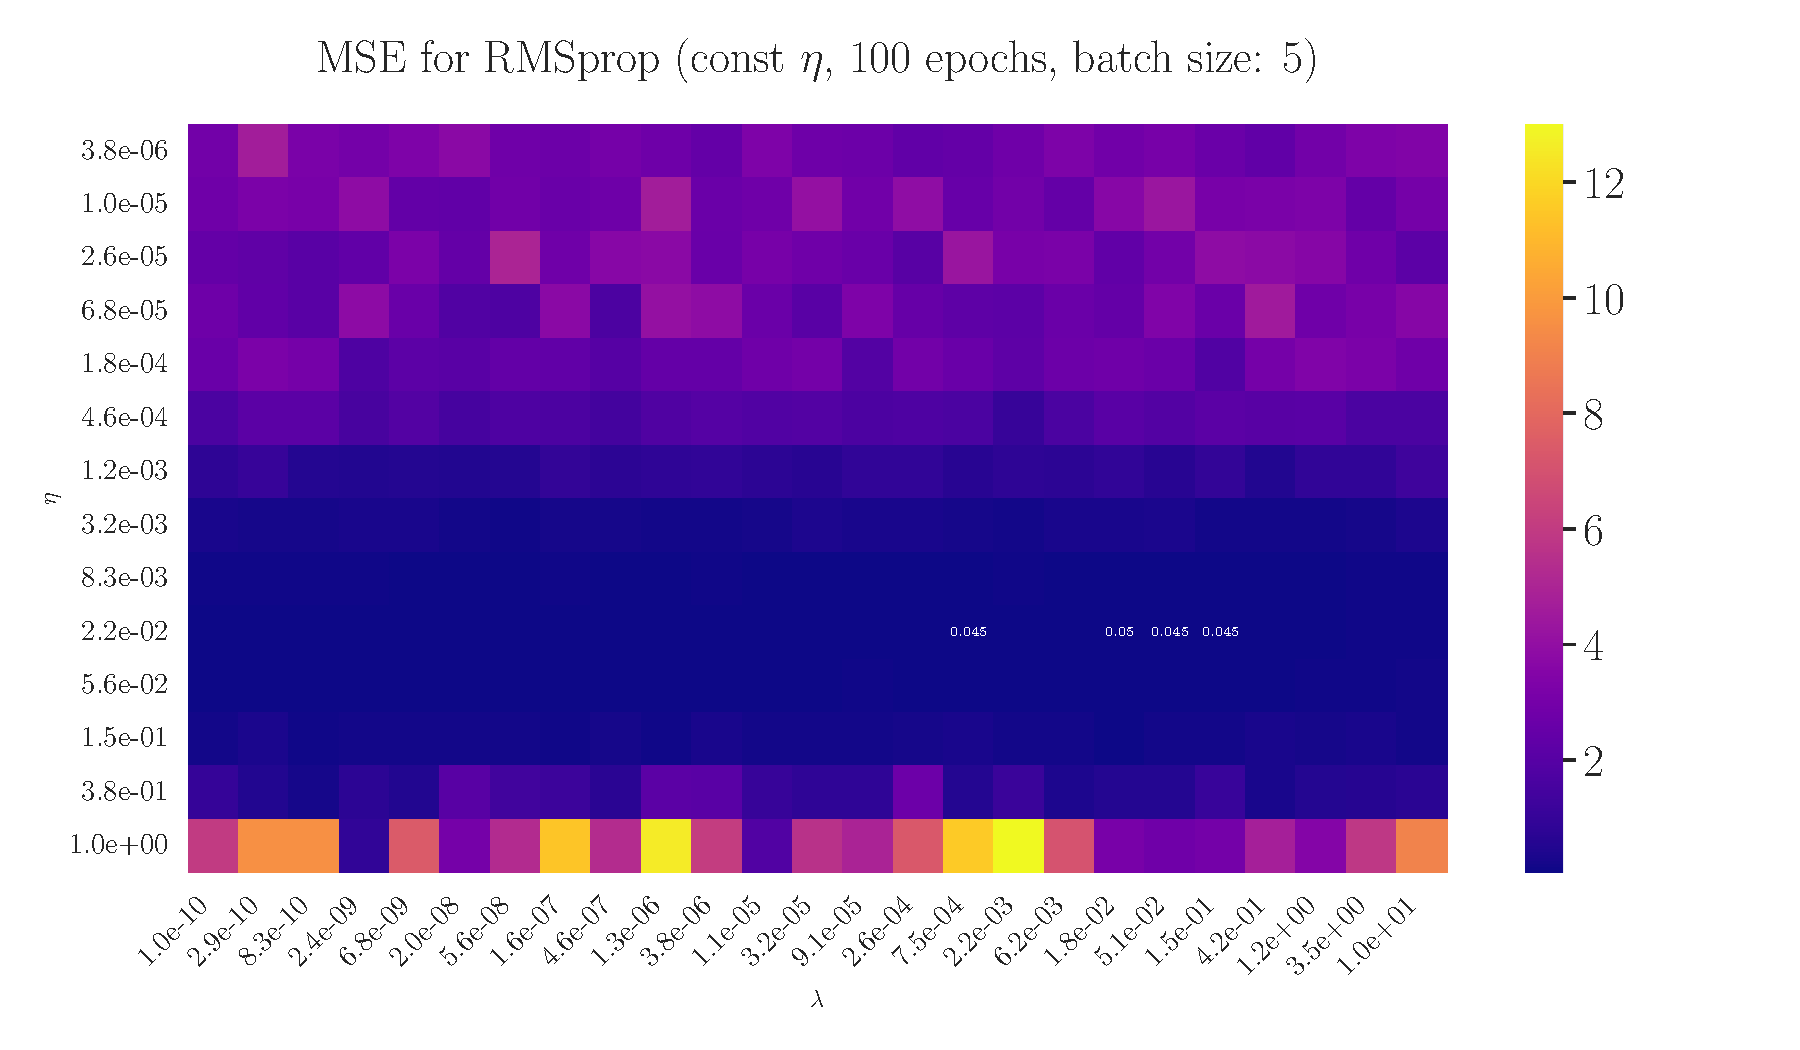
\includegraphics[width=\textwidth]{Figures/LinRegRMSprop_constEta_100epochs_batchS5.pdf}
% 		\caption{\(100\) epochs and a batch size of \(5\).}
% 		\label{fig:LinRegRMSprop_constEta_100epochs_5batchS}
% 	\end{subfigure}
% \hfill\newline
% \begin{subfigure}{0.41\textwidth}
% 	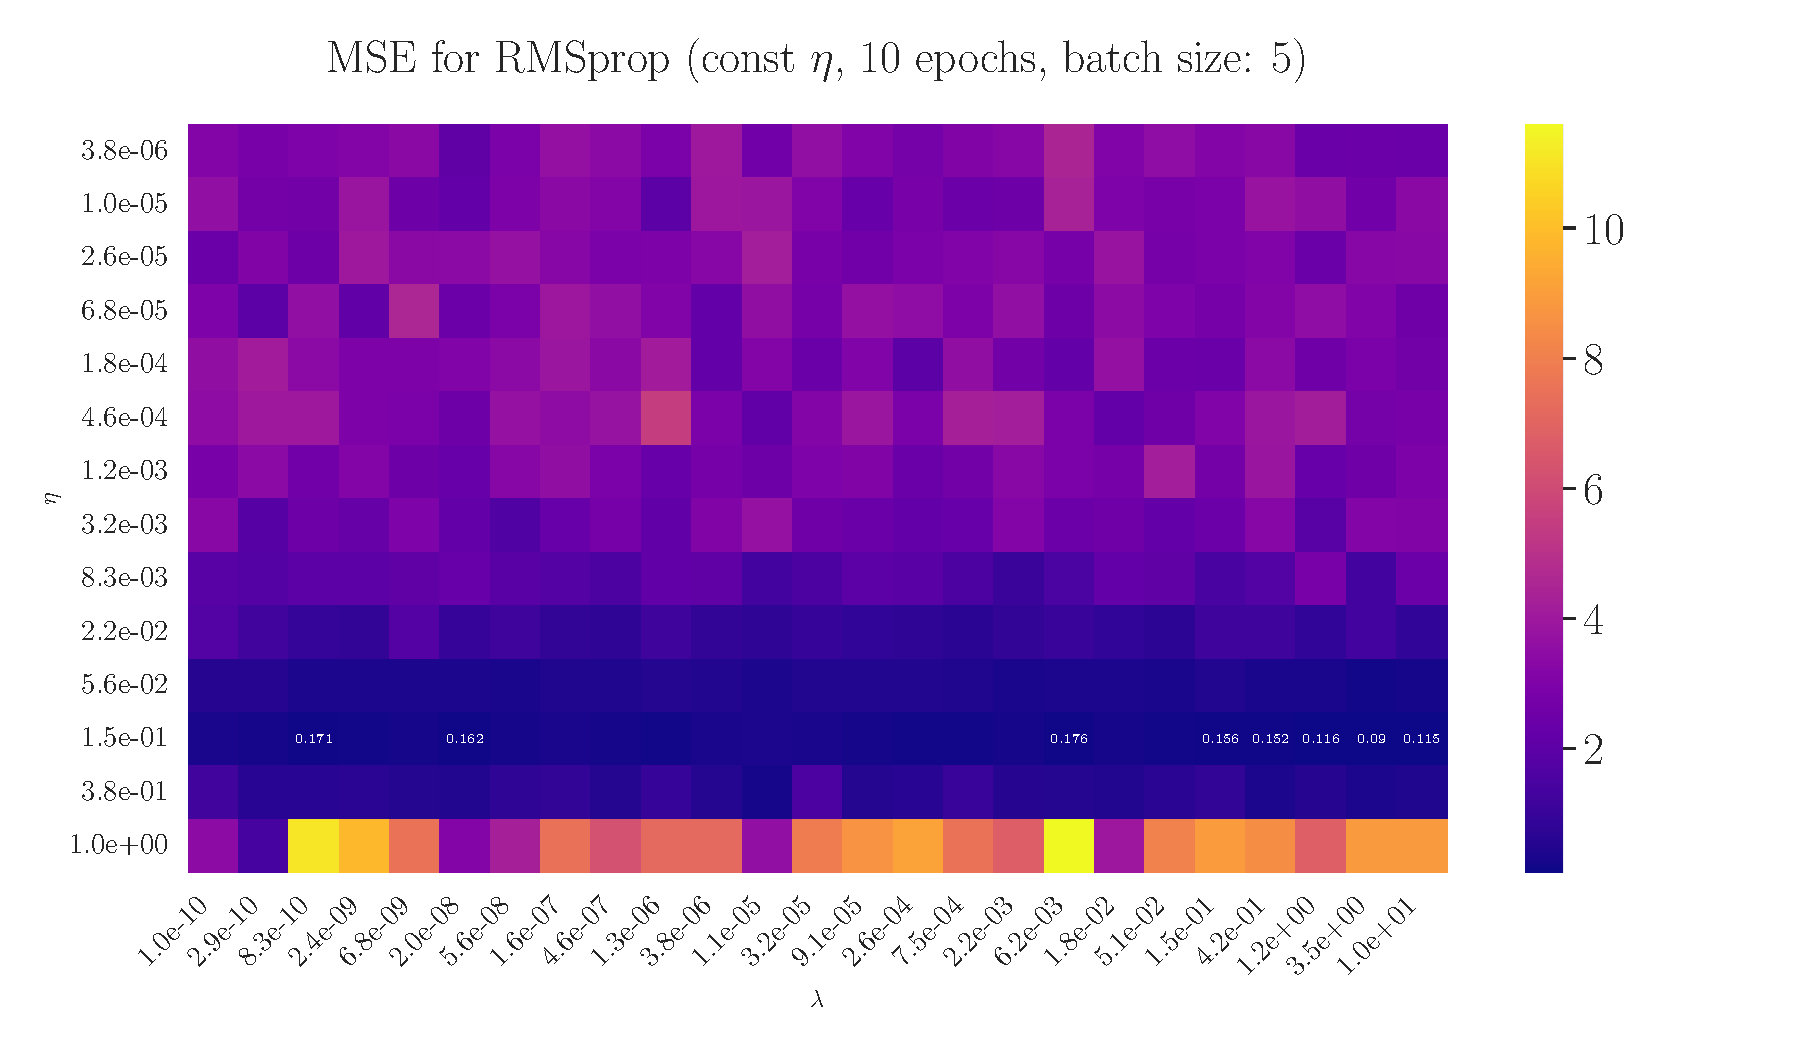
\includegraphics[width=\textwidth]{Figures/LinRegRMSprop_constEta_10epochs_batchS10.pdf}
% 	\caption{\(10\) epochs and a batch size of \(10\).}
% 	\label{fig:LinRegRMSprop_constEta_10epochs_5batchS}
% \end{subfigure}
% \hfill
% \begin{subfigure}{0.41\textwidth}
% 	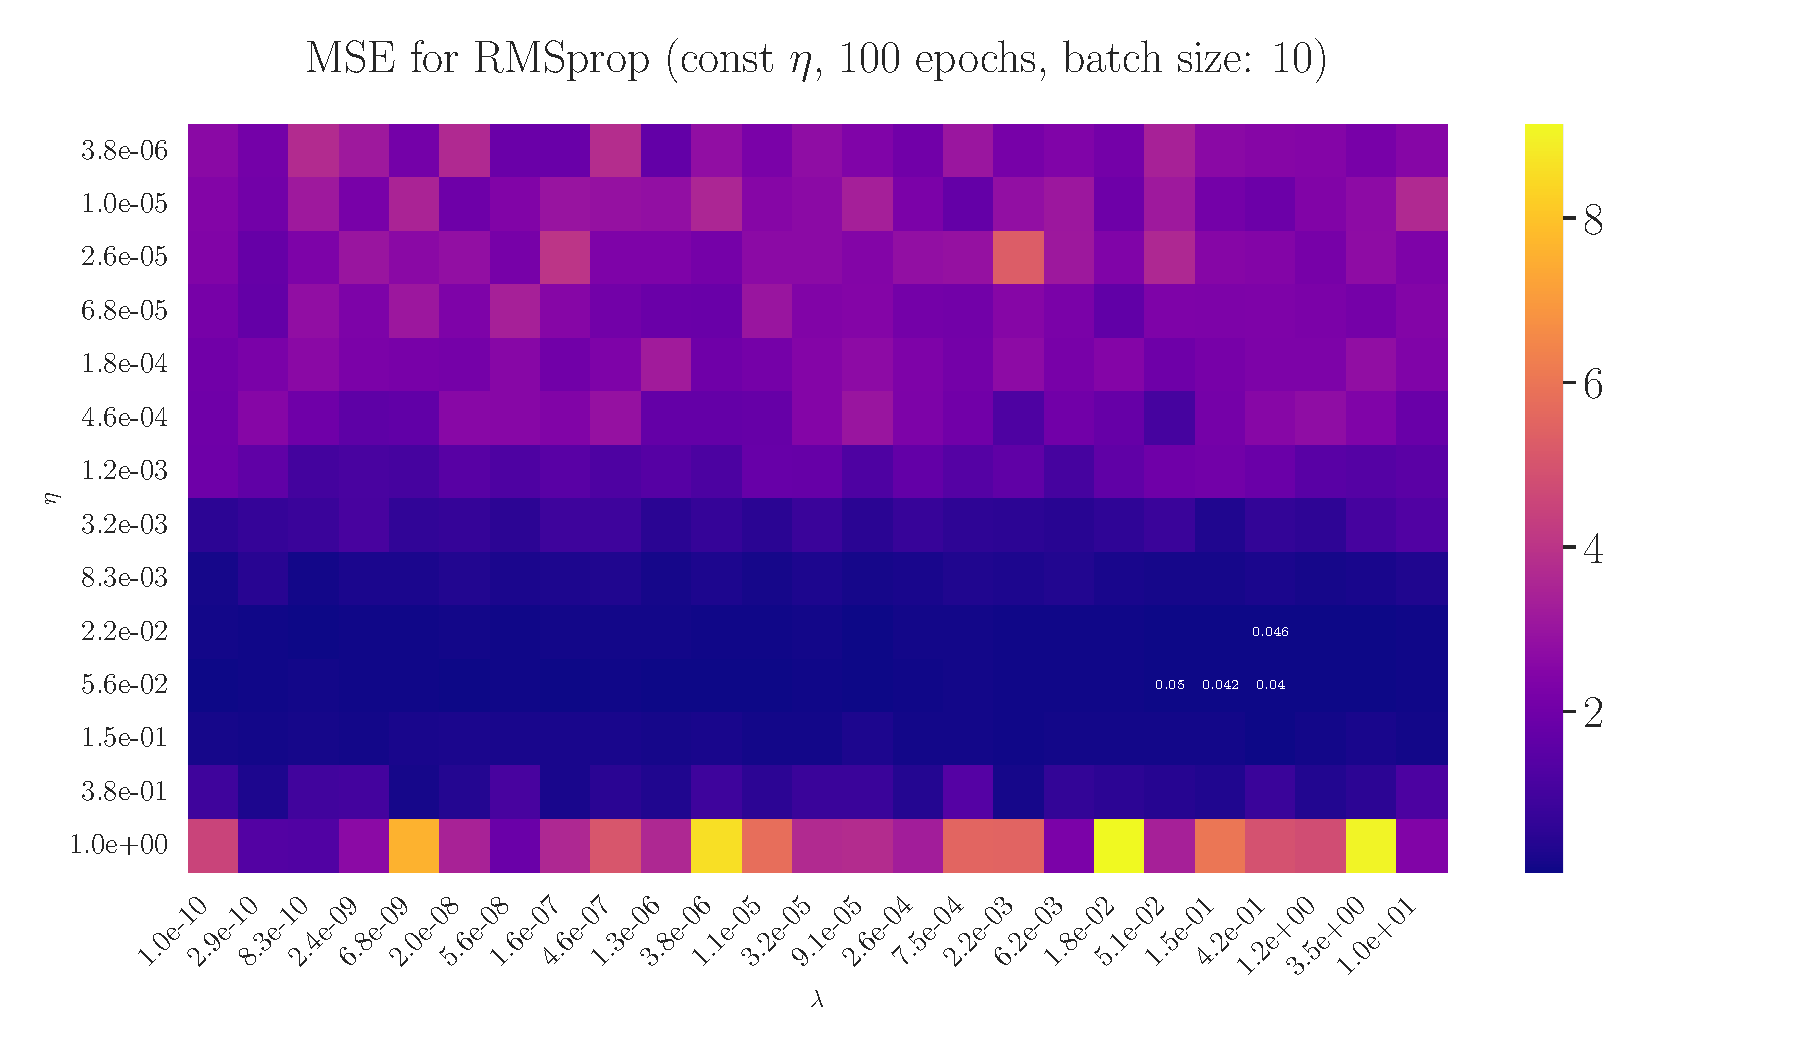
\includegraphics[width=\textwidth]{Figures/LinRegRMSprop_constEta_100epochs_batchS10.pdf}
% 	\caption{\(100\) epochs and a batch size of \(10\).}
% 	\label{fig:LinRegRMSprop_constEta_100epochs_5batchS}
% \end{subfigure}
% \caption{MSE scores using RMSprop with a constant learning rate.}
% \label{fig:RMSprop_constEta}
% \end{figure*}


% % AdaGrad with varying learning rate
% \begin{figure*}
% 	\begin{subfigure}{0.41\textwidth}
% 		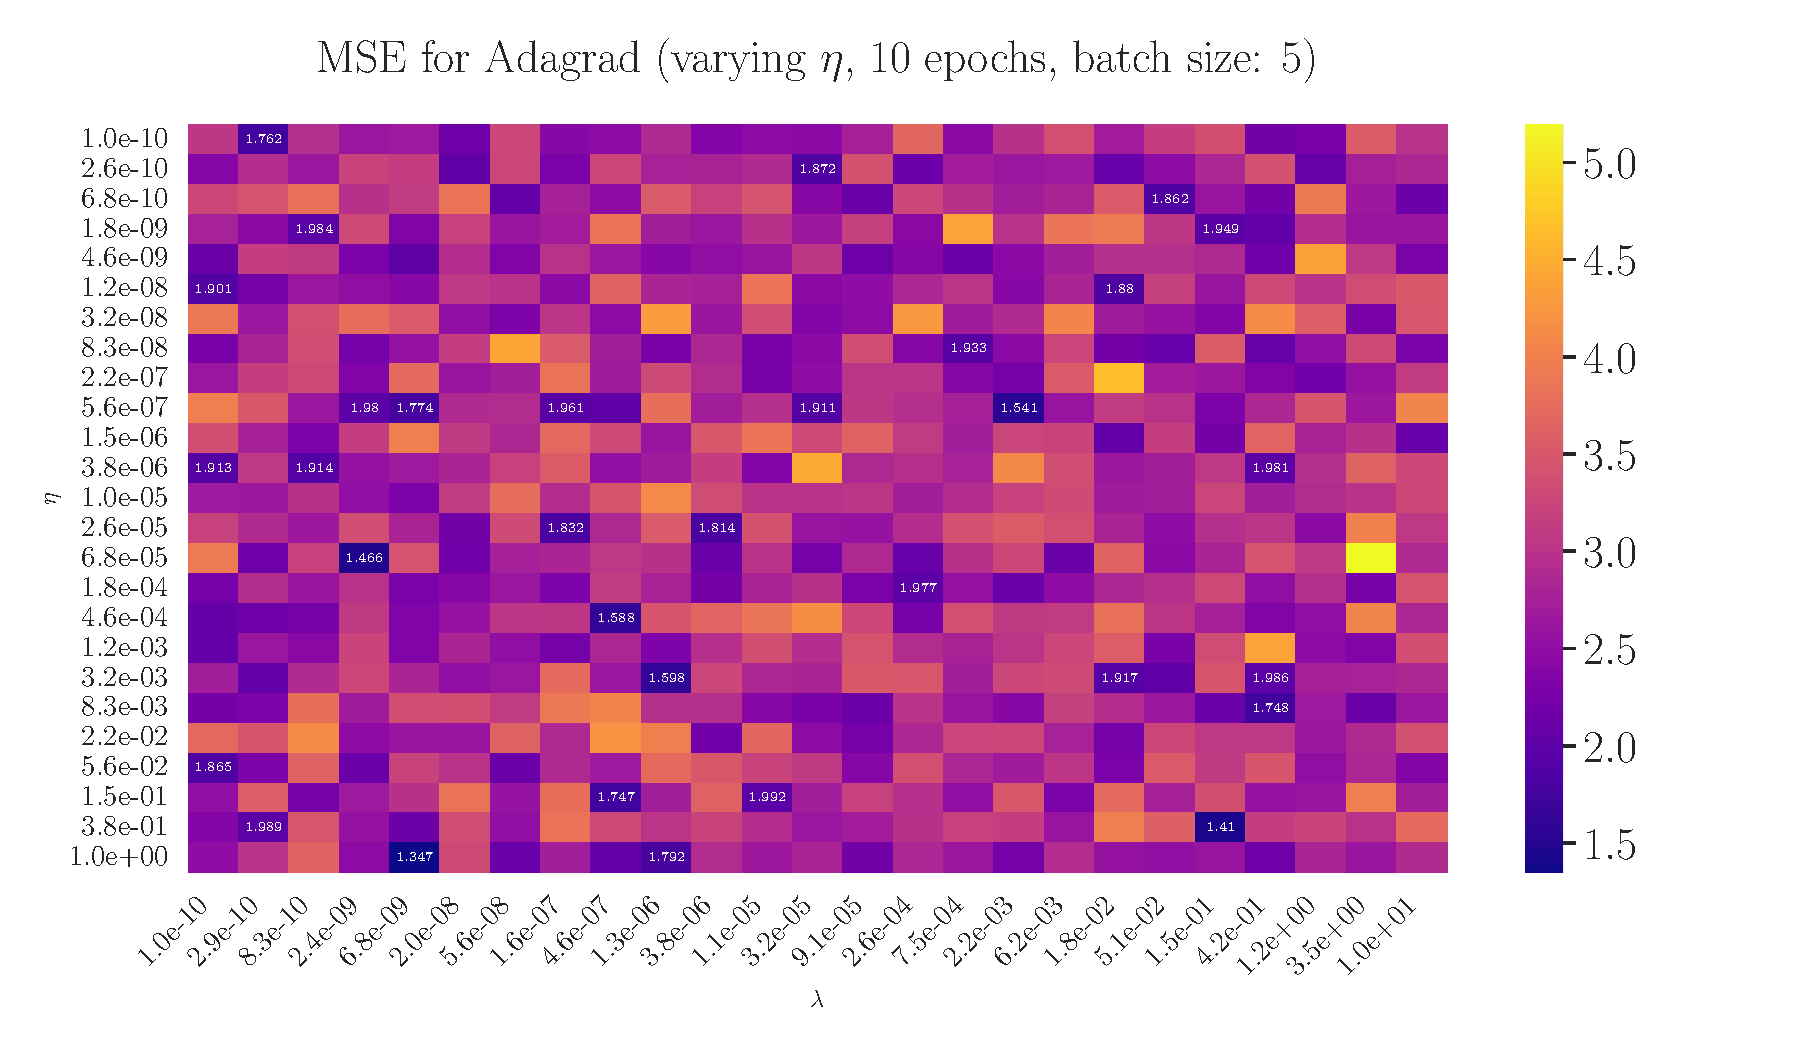
\includegraphics[width=\textwidth]{Figures/LinRegAdaGrad_varyEta_10epochs_batchS5.pdf}
% 		\caption{\(10\) epochs and a batch size of \(5\).}
% 		\label{fig:LinRegAdaGrad_varyEta_10epochs_5batchS}
% 	\end{subfigure}
% 	\hfill
% 	\begin{subfigure}{0.41\textwidth}
% 		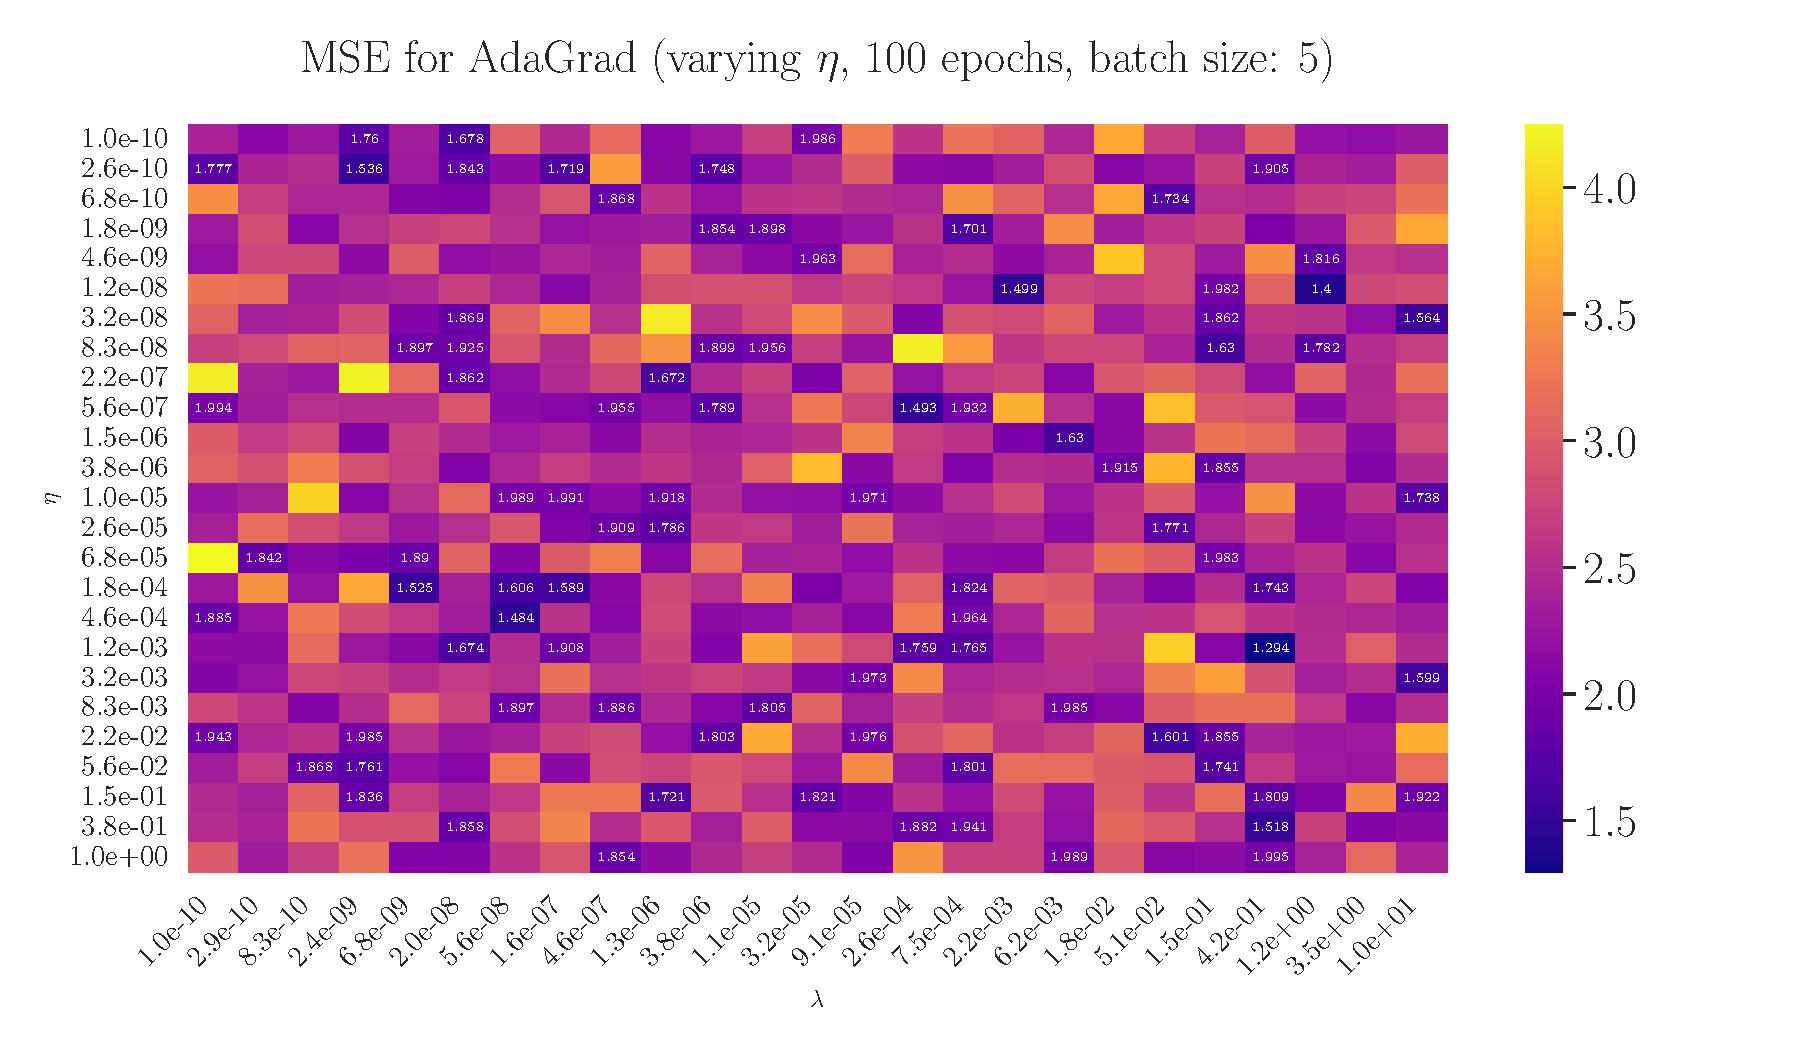
\includegraphics[width=\textwidth]{Figures/LinRegAdaGrad_varyEta_100epochs_batchS5.pdf}
% 		\caption{\(100\) epochs and a batch size of \(5\).}
% 		\label{fig:LinRegAdaGrad_varyEta_100epochs_5batchS}
% 	\end{subfigure}
% \hfill\newline
% \begin{subfigure}{0.41\textwidth}
% 	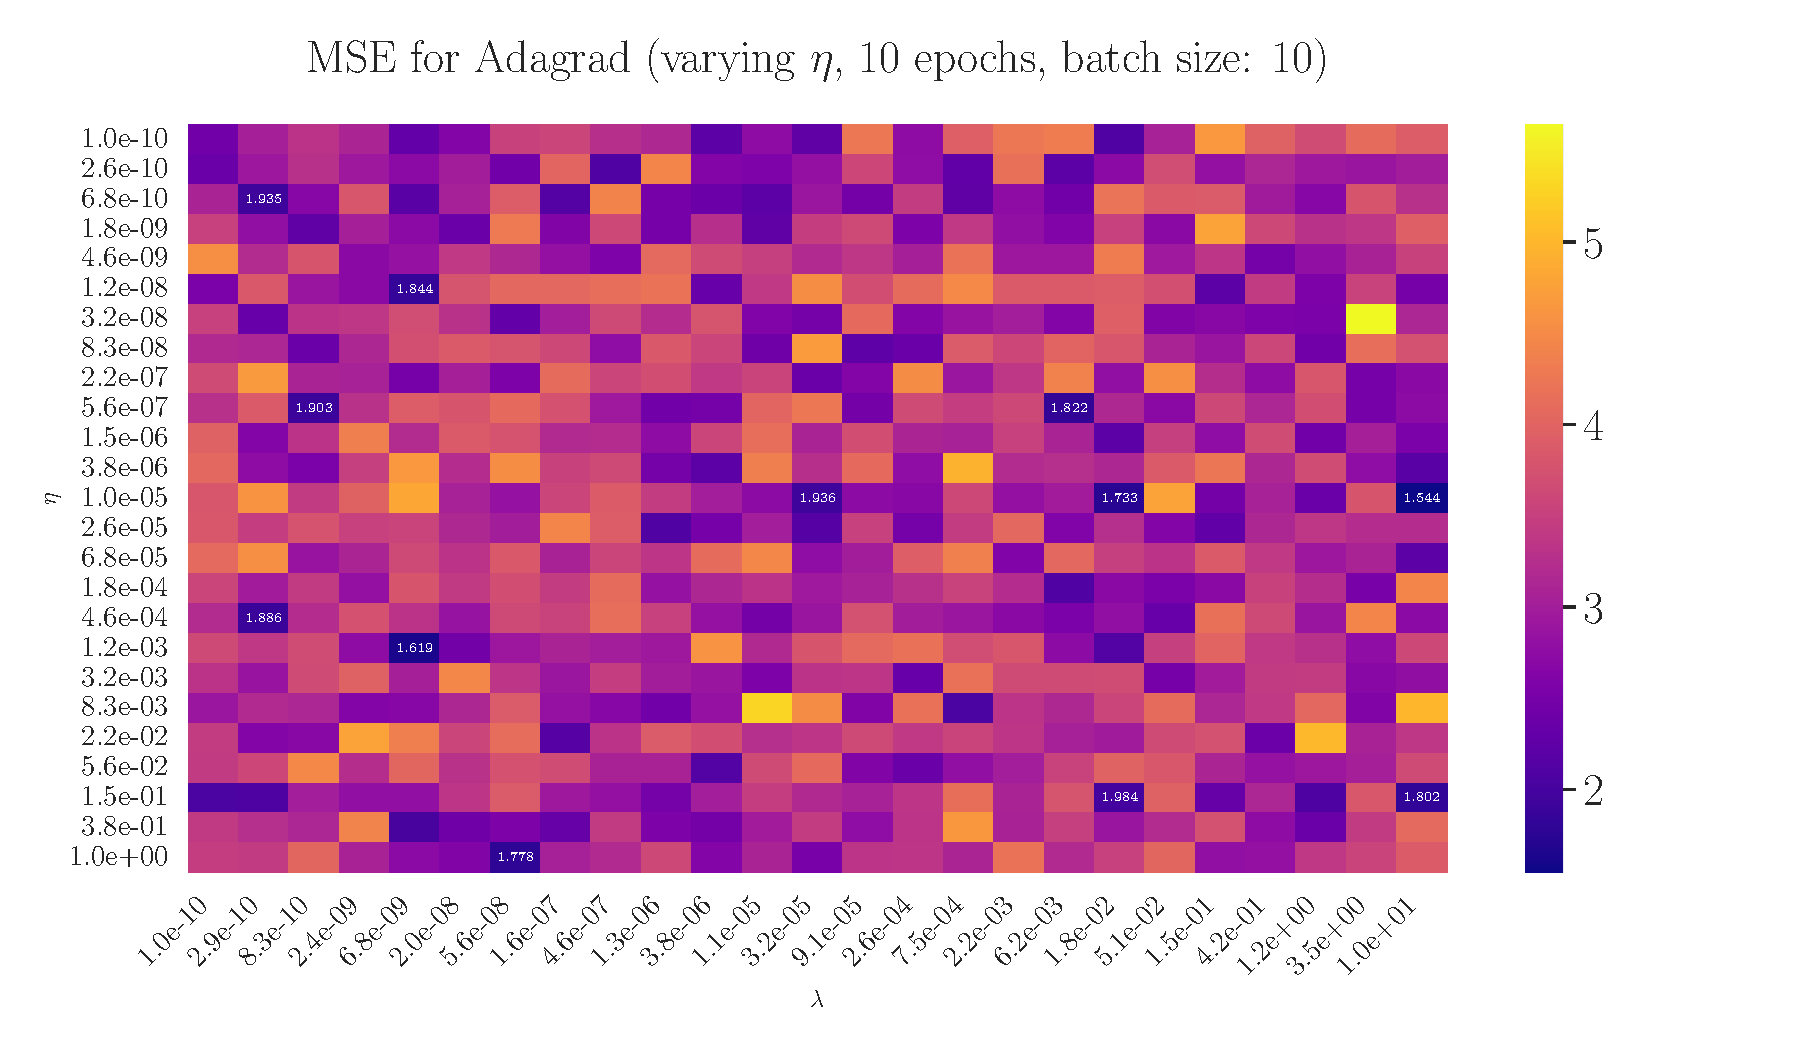
\includegraphics[width=\textwidth]{Figures/LinRegAdaGrad_varyEta_10epochs_batchS10.pdf}
% 	\caption{\(10\) epochs and a batch size of \(10\).}
% 	\label{fig:LinRegAdaGrad_varyEta_10epochs_5batchS}
% \end{subfigure}
% \hfill
% \begin{subfigure}{0.41\textwidth}
% 	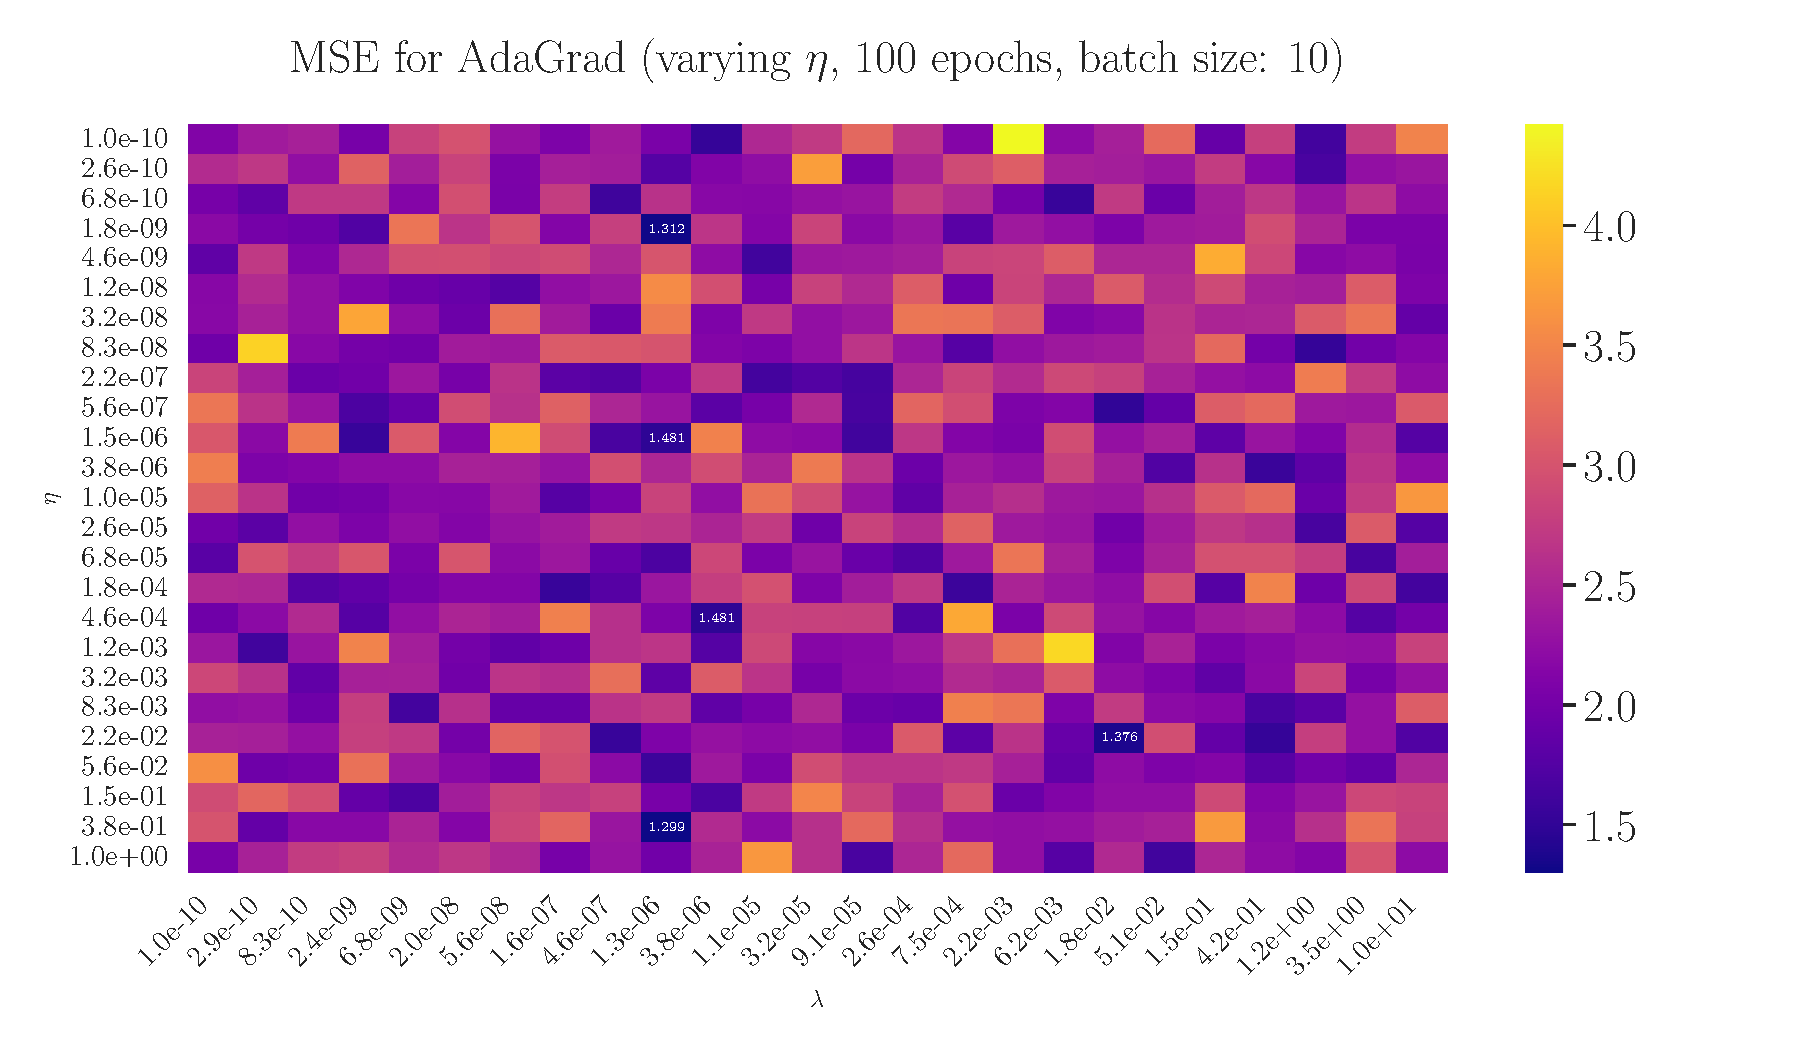
\includegraphics[width=\textwidth]{Figures/LinRegAdaGrad_varyEta_100epochs_batchS10.pdf}
% 	\caption{\(100\) epochs and a batch size of \(10\).}
% 	\label{fig:LinRegAdaGrad_varyEta_100epochs_5batchS}
% \end{subfigure}
% \caption{MSE scores using AdaGrad with a varying learning rate; see \eqref{eq:varyin_learning_rate}, \(t_0=2\) and \(t_1=\eta\), where \(\eta\) can be read from the y-axis.}
% \label{fig:AdaGrad_varyEta}
% \end{figure*}

% % AdaGrad with constant learning rate
% \begin{figure*}
% 	\begin{subfigure}{0.41\textwidth}
% 		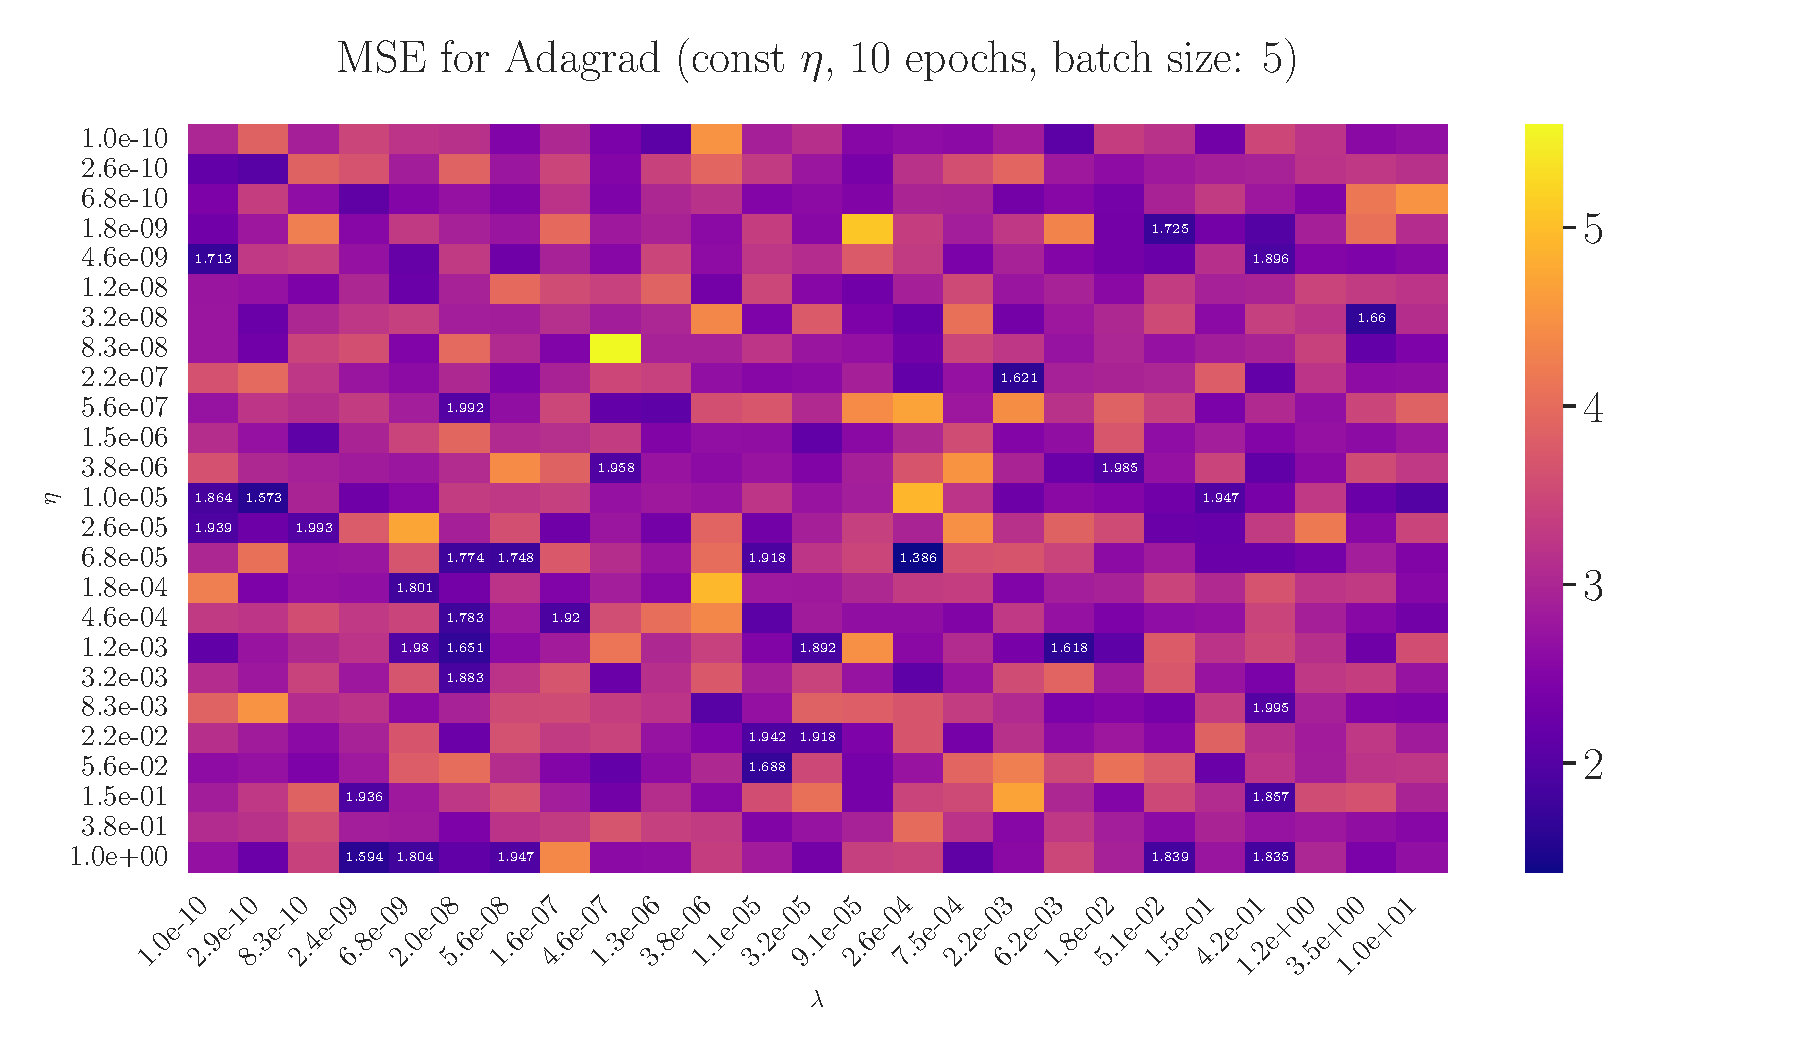
\includegraphics[width=\textwidth]{Figures/LinRegAdaGrad_constEta_10epochs_batchS5.pdf}
% 		\caption{\(10\) epochs and a batch size of \(5\).}
% 		\label{fig:LinRegAdaGrad_constEta_10epochs_5batchS}
% 	\end{subfigure}
% 	\hfill
% 	\begin{subfigure}{0.41\textwidth}
% 		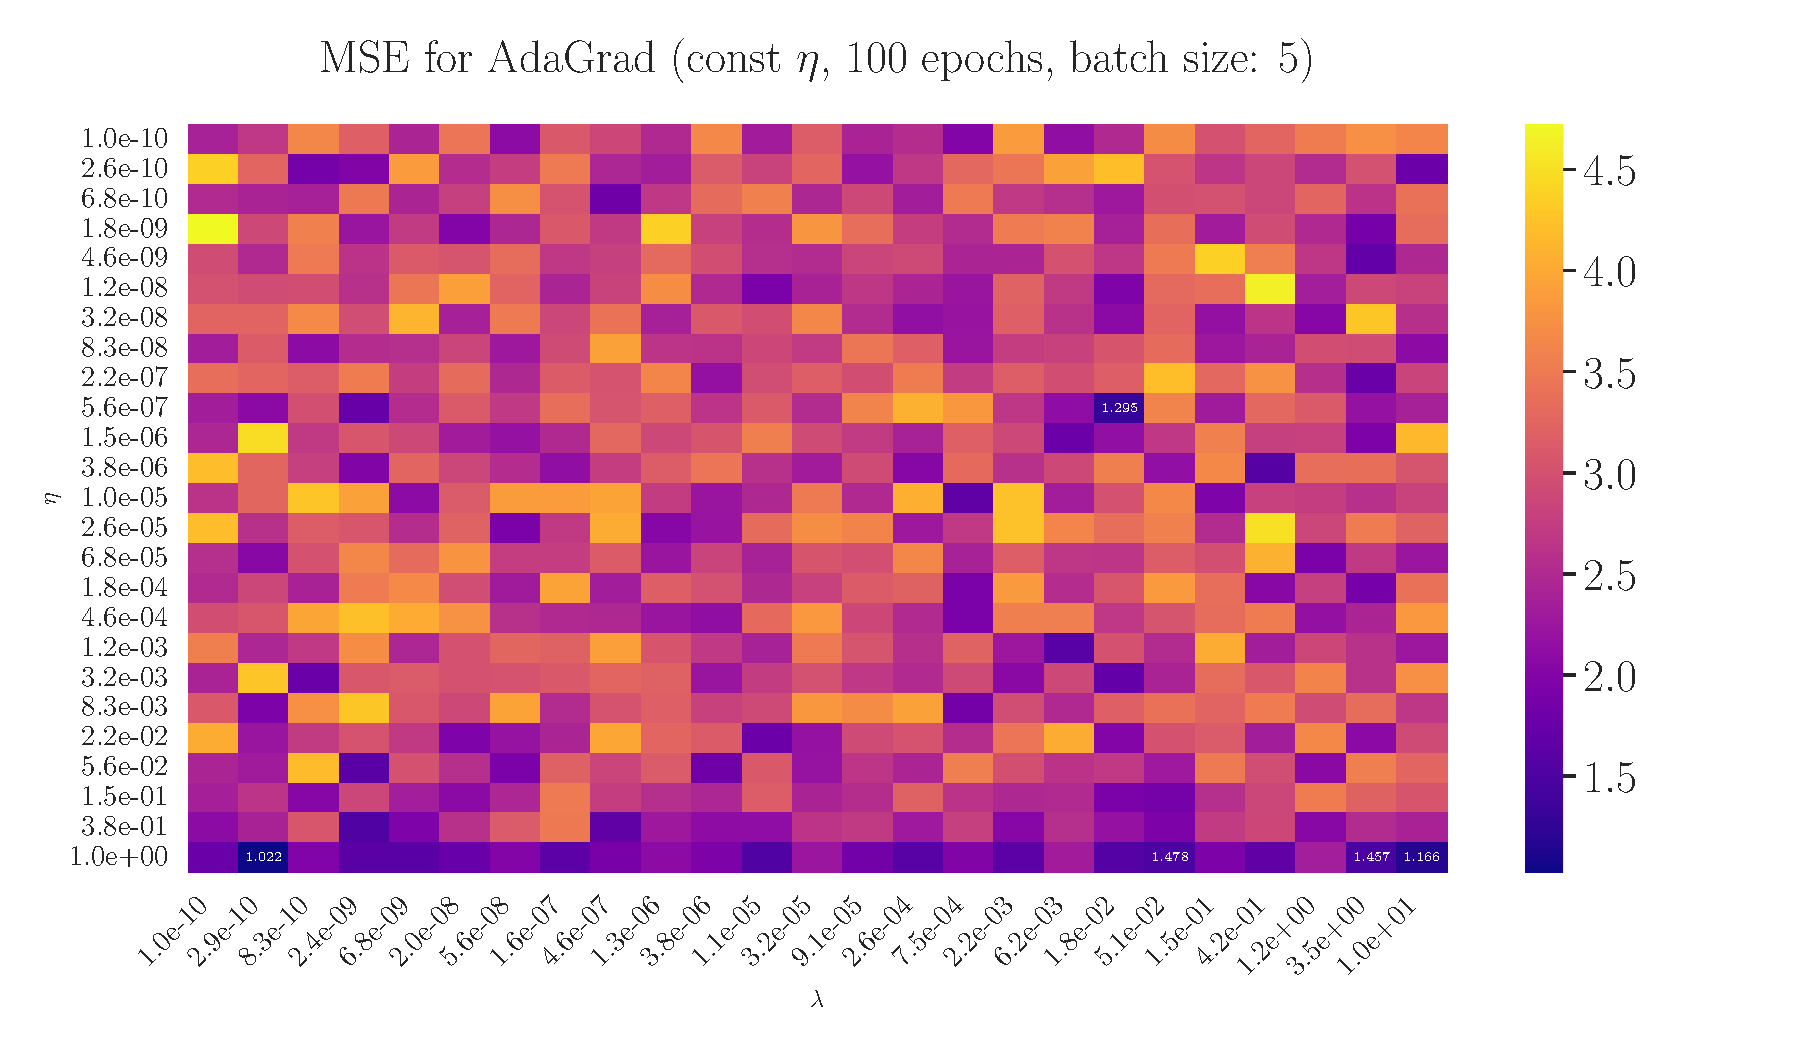
\includegraphics[width=\textwidth]{Figures/LinRegAdaGrad_constEta_100epochs_batchS5.pdf}
% 		\caption{\(100\) epochs and a batch size of \(5\).}
% 		\label{fig:LinRegAdaGrad_constEta_100epochs_5batchS}
% 	\end{subfigure}
% \hfill\newline
% \begin{subfigure}{0.41\textwidth}
% 	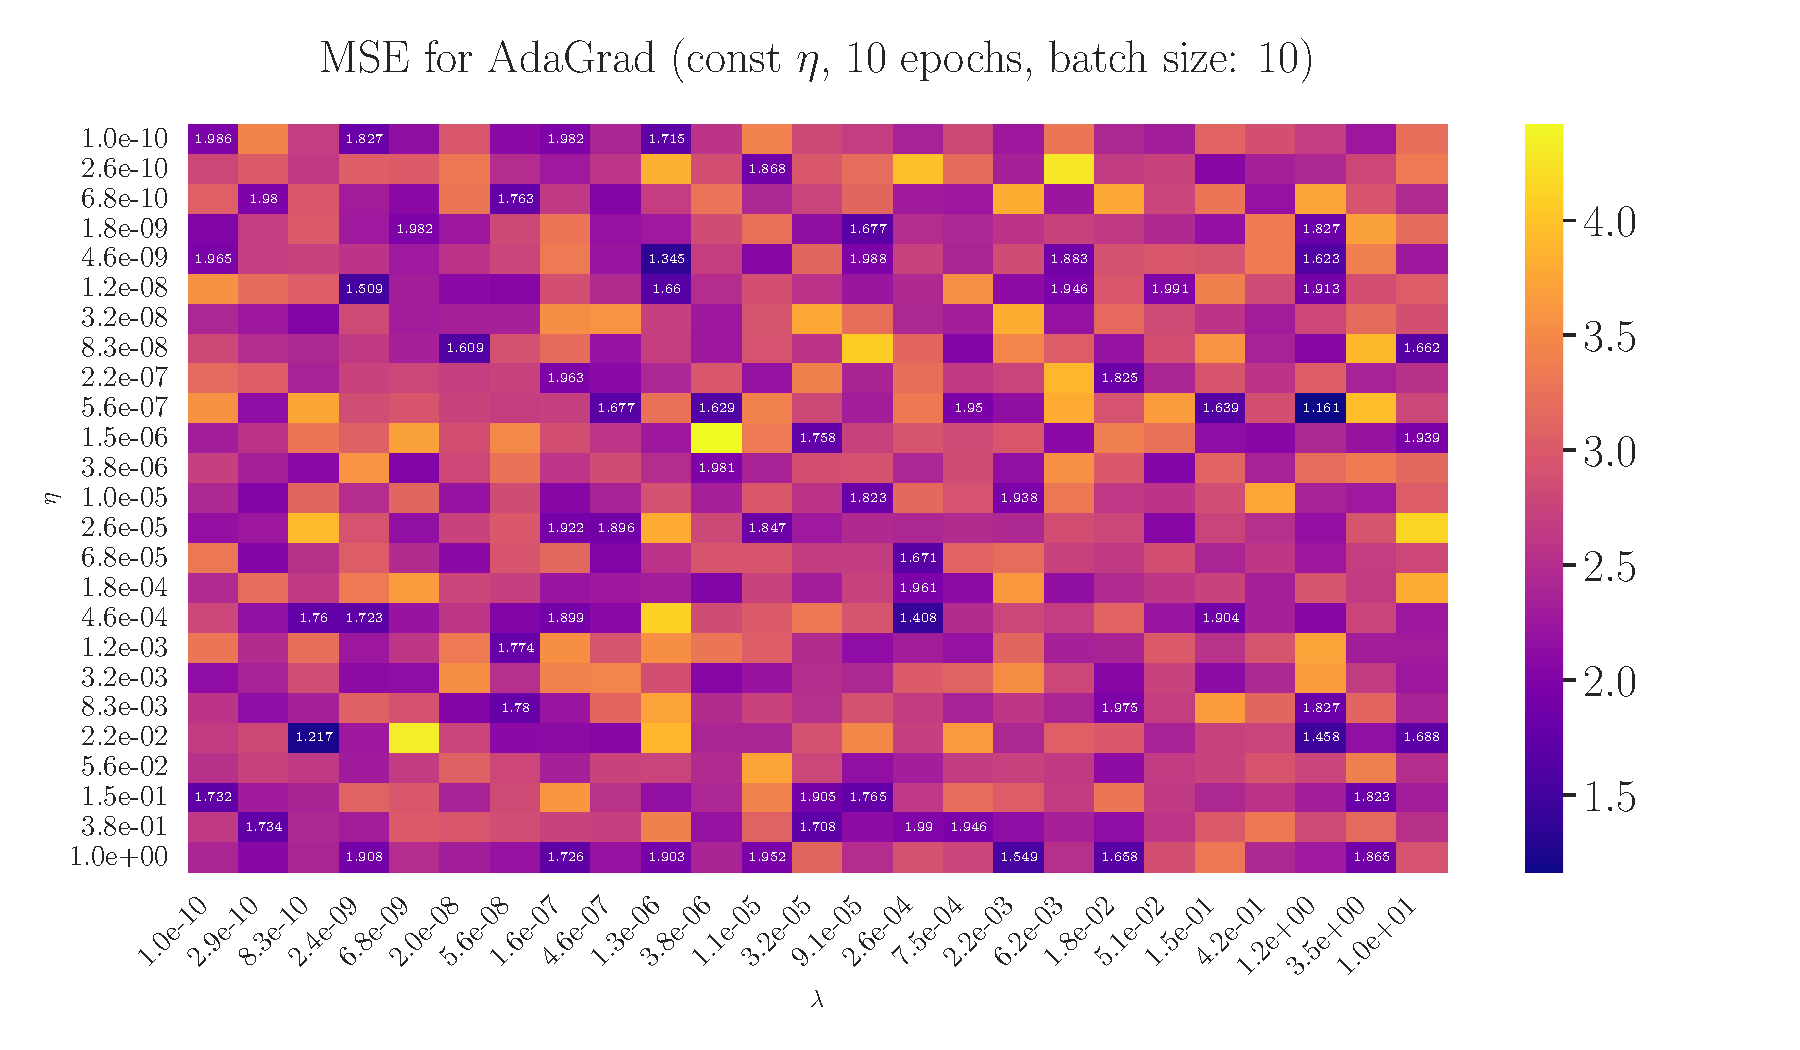
\includegraphics[width=\textwidth]{Figures/LinRegAdaGrad_constEta_10epochs_batchS10.pdf}
% 	\caption{\(10\) epochs and a batch size of \(10\).}
% 	\label{fig:LinRegAdaGrad_constEta_10epochs_5batchS}
% \end{subfigure}
% \hfill
% \begin{subfigure}{0.41\textwidth}
% 	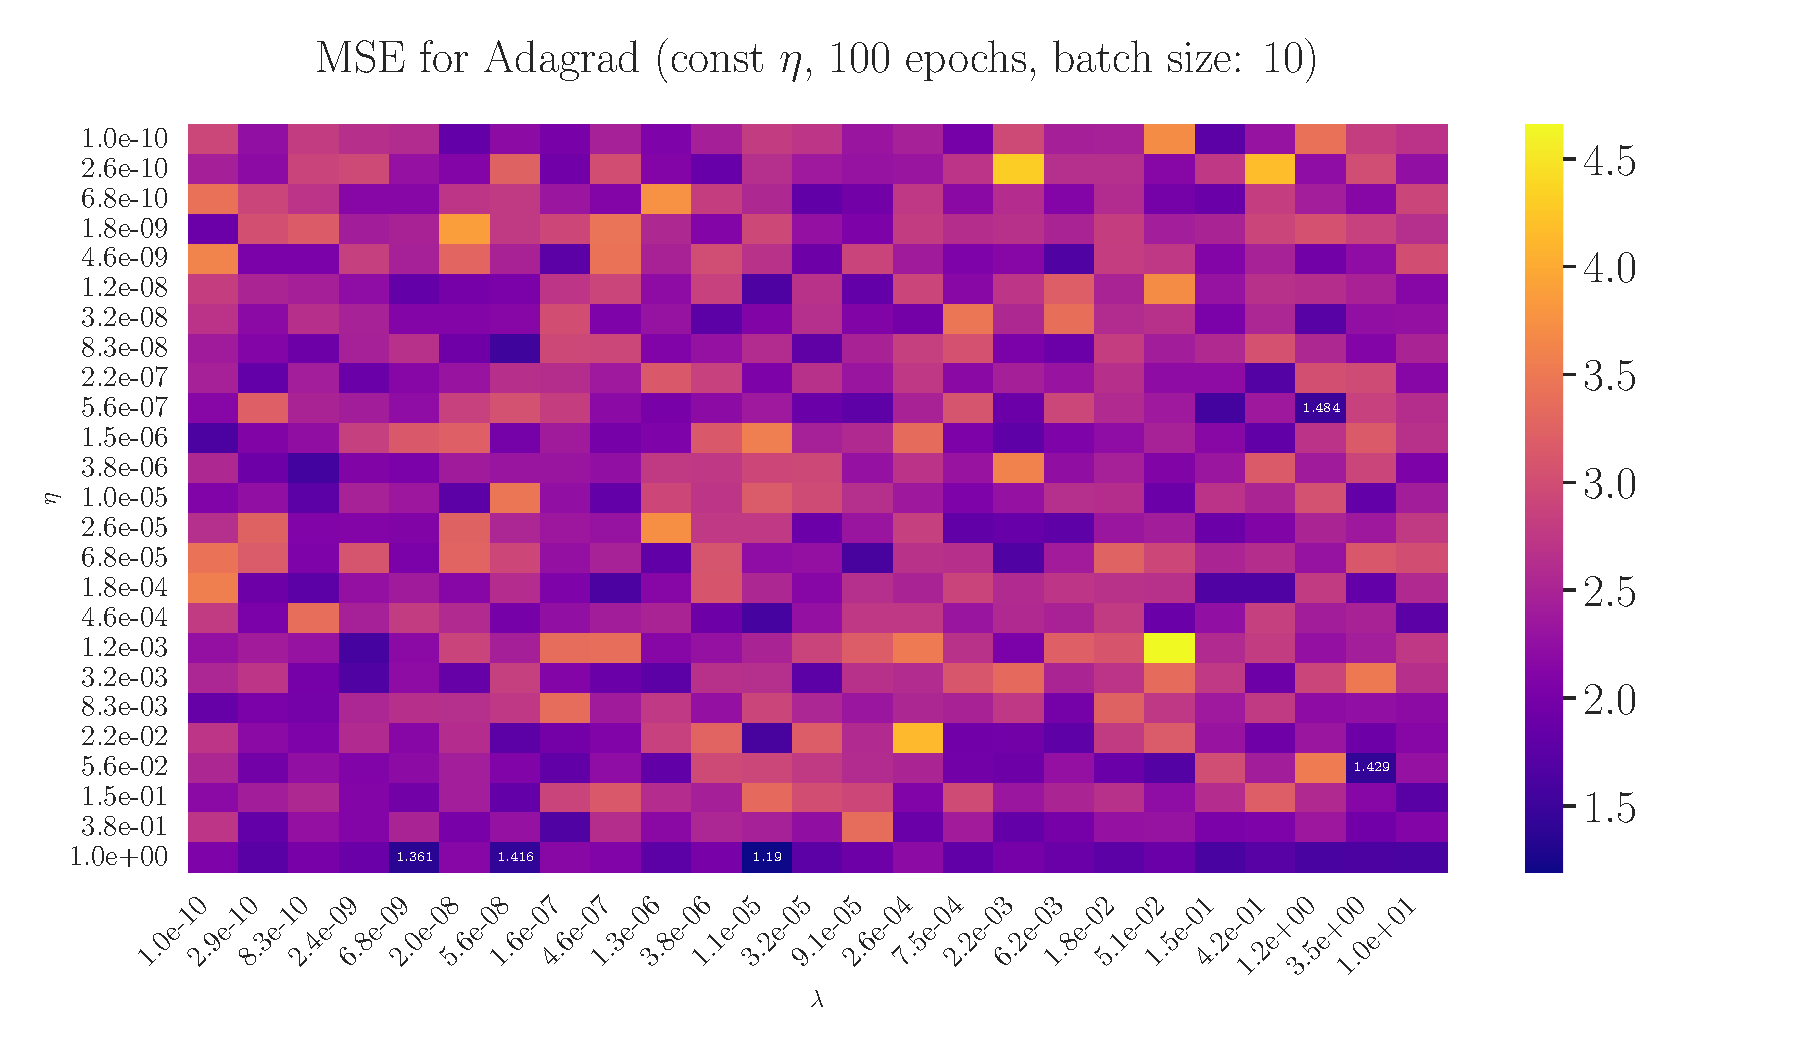
\includegraphics[width=\textwidth]{Figures/LinRegAdaGrad_constEta_100epochs_batchS10.pdf}
% 	\caption{\(100\) epochs and a batch size of \(10\).}
% 	\label{fig:LinRegAdaGrad_constEta_100epochs_5batchS}
% \end{subfigure}
% \caption{MSE scores using AdaGrad with a constant learning rate.}
% \label{fig:AdaGrad_constEta}
% \end{figure*}

% % Adam with varying learning rate
% \begin{figure*}
% 	\begin{subfigure}{0.41\textwidth}
% 		\includegraphics[width=\textwidth]{Figures/LinRegAdam_varyEta_10epochs_batchS5.pdf}
% 		\caption{\(10\) epochs and a batch size of \(5\).}
% 		\label{fig:LinRegAdam_varyEta_10epochs_5batchS}
% 	\end{subfigure}
% 	\hfill
% 	\begin{subfigure}{0.41\textwidth}
% 		\includegraphics[width=\textwidth]{Figures/LinRegAdam_varyEta_100epochs_batchS5.pdf}
% 		\caption{\(100\) epochs and a batch size of \(5\).}
% 		\label{fig:LinRegAdam_varyEta_100epochs_5batchS}
% 	\end{subfigure}
% \hfill\newline
% \begin{subfigure}{0.41\textwidth}
% 	\includegraphics[width=\textwidth]{Figures/LinRegAdam_varyEta_10epochs_batchS10.pdf}
% 	\caption{\(10\) epochs and a batch size of \(10\).}
% 	\label{fig:LinRegAdam_varyEta_10epochs_5batchS}
% \end{subfigure}
% \hfill
% \begin{subfigure}{0.41\textwidth}
% 	\includegraphics[width=\textwidth]{Figures/LinRegAdam_varyEta_100epochs_batchS10.pdf}
% 	\caption{\(100\) epochs and a batch size of \(10\).}
% 	\label{fig:LinRegAdam_varyEta_100epochs_5batchS}
% \end{subfigure}
% \caption{MSE scores using Adam with a varying learning rate; see \eqref{eq:varyin_learning_rate}, \(t_0=2\) and \(t_1=\eta\), where \(\eta\) can be read from the y-axis.}
% \label{fig:Adam_varyEta}
% \end{figure*}

% % Adam with constant learning rate
% \begin{figure*}
% 	\begin{subfigure}{0.41\textwidth}
% 		\includegraphics[width=\textwidth]{Figures/LinRegAdam_constEta_10epochs_batchS5.pdf}
% 		\caption{\(10\) epochs and a batch size of \(5\).}
% 		\label{fig:LinRegAdam_constEta_10epochs_5batchS}
% 	\end{subfigure}
% 	\hfill
% 	\begin{subfigure}{0.41\textwidth}
% 		\includegraphics[width=\textwidth]{Figures/LinRegAdam_constEta_100epochs_batchS5.pdf}
% 		\caption{\(100\) epochs and a batch size of \(5\).}
% 		\label{fig:LinRegAdam_constEta_100epochs_5batchS}
% 	\end{subfigure}
% \hfill\newline
% \begin{subfigure}{0.41\textwidth}
% 	\includegraphics[width=\textwidth]{Figures/LinRegAdam_constEta_10epochs_batchS10.pdf}
% 	\caption{\(10\) epochs and a batch size of \(10\).}
% 	\label{fig:LinRegAdam_constEta_10epochs_5batchS}
% \end{subfigure}
% \hfill
% \begin{subfigure}{0.41\textwidth}
% 	\includegraphics[width=\textwidth]{Figures/LinRegAdam_constEta_100epochs_batchS10.pdf}
% 	\caption{\(100\) epochs and a batch size of \(10\).}
% 	\label{fig:LinRegAdam_constEta_100epochs_5batchS}
% \end{subfigure}
% \caption{MSE scores using Adam with a constant learning rate.}
% \label{fig:Adam_constEta}
% \end{figure*}

\end{document}